\documentclass{article}
\usepackage[utf8]{inputenc}
\usepackage[T5]{fontenc} % sử dụng tiếng Việt
\usepackage[fontsize=13pt]{scrextend} % chỉnh font size = 13pt
\usepackage[paperheight = 29.7cm, paperwidth = 21cm, right = 2cm, left = 3cm, top = 2cm, bottom = 2.5cm]{geometry} % Chuẩn A4, căn lề trái phải trên dưới
\usepackage{graphicx}
\usepackage{float}
\usepackage{tikz}
\usepackage{indentfirst}
\usetikzlibrary{calc}
\renewcommand{\baselinestretch}{1.5}
\setlength{\parskip}{6pt}
\setlength{\parindent}{1cm}
\usepackage{titlesec}
% Required packages
\usepackage{color}
\usepackage{xcolor}
\usepackage{listings}
\usepackage{algorithm}
\usepackage{algorithmic}
\usepackage{enumitem}
\usepackage{listings}
\usepackage{amsmath}
\usepackage{algorithm}
\usepackage[noend]{algpseudocode}
\usepackage{tabularx}
\usepackage{tabularray}
\usepackage{longtable}
\usepackage{hyperref}
\usepackage{url}
\usepackage{cite}
\renewcommand{\labelenumi}{[\arabic{enumi}]}
\usepackage{algorithm,algpseudocode}
\usepackage{lipsum}

\usepackage{enotez}
\usepackage{adjustbox} % Add this package if not already included

\setlength{\tabcolsep}{3pt}

% Configure enotez for Vietnamese
\setenotez{
    list-name = {},
    backref = true,  % Enable back-references
    totoc = false,   % Don't add to table of contents
    reset = true,
}

\usepackage{footmisc}
\setlength{\footnotesep}{12pt}
\renewcommand{\footnoterule}{\vspace*{-3pt}\hrule width 2in height 0.4pt \vspace*{2.6pt}}

% Make footnotes ragged right for better line breaks
\makeatletter
\renewcommand\@makefntext[1]{%
  \parindent 1em%
  \noindent
  \hb@xt@1.8em{\hss\@makefnmark}%
  \raggedright #1}
\makeatothers

\newcommand{\nocontentsline}[3]{}
\newcommand{\tocless}[2]{\bgroup\let\addcontentsline=\nocontentsline#1{#2}\egroup}

\makeatletter
\newenvironment{breakablealgorithm}
  {% \begin{breakablealgorithm}
   \begin{center}
     \vspace{10pt}
     \refstepcounter{algorithm}% New algorithm
     \hrule height.8pt depth0pt \kern2pt% \@fs@pre for \@fs@ruled
     \renewcommand{\caption}[2][\relax]{% Make a new \caption
       {\raggedright\textbf{\fname@algorithm~\thealgorithm} ##2\par}%
       \ifx\relax##1\relax % #1 is \relax
         \addcontentsline{loa}{algorithm}{\protect\numberline{\thealgorithm}##2}%
       \else % #1 is not \relax
         \addcontentsline{loa}{algorithm}{\protect\numberline{\thealgorithm}##1}%
       \fi
       \kern2pt\hrule\kern2pt
     }
  }{% \end{breakablealgorithm}
     \kern2pt\hrule\relax% \@fs@post for \@fs@ruled
   \end{center}
  }
\makeatother
\makeatletter
\def\BState{\State\hskip-\ALG@thistlm}
\makeatother

\makeatletter
\def\BState{\State\hskip-\ALG@thistlm}
\makeatother

\hypersetup{
    colorlinks=true,
    linkcolor=black,        % Keep TOC and section links black
    citecolor=black,        % Keep citations black
    urlcolor=blue,          % URLs stay blue
    filecolor=blue
}

\makeatletter
% Only affect List of Figures, not TOC
\renewcommand*\l@figure{\@dottedtocline{1}{1.5em}{3.5em}}
\makeatother

\titlespacing*{\section}{0pt}{0pt}{30pt} %heading 1
\titleformat*{\section}{\fontsize{24pt}{0pt}\selectfont \bfseries \centering}

\titlespacing{\subsection}{0pt}{10pt}{0pt} %heading 2
\titleformat{\subsection}{\fontsize{14pt}{0pt}\selectfont \bfseries}

\titlespacing{\subsubsection}{0pt}{10pt}{0pt} %heading 2
\titleformat{\subsubsection}{\fontsize{13pt}{0pt}\selectfont \bfseries \itshape}

\titlespacing{\paragraph}{0pt}{10pt}{0pt} %heading 3
\titleformat{\paragraph}{\normalfont\normalsize\bfseries}{\theparagraph}{1em}{}

\renewcommand{\figurename}{\fontsize{12pt}{0pt}\selectfont \itshape Hình}
\renewcommand{\thefigure}{\thesection.\arabic{figure}}
\usepackage{caption}
\captionsetup[figure]{labelsep=space}

\renewcommand{\tablename}{\fontsize{12pt}{0pt}\selectfont \itshape Bảng}
\renewcommand{\thetable}{\thesection.\arabic{table}}
\captionsetup[table]{labelsep=space}

\begin{document}

\begin{titlepage}

% vẽ khung
\begin{tikzpicture} [overlay, remember picture]
\draw [line width = 3pt]
    ($ (current page.north west) + (3.0cm, -2.0cm) $)
    rectangle
    ($ (current page.south east) + (-2.0cm, 2.5cm) $);
\draw[line width = 0.5 pt]
    ($ (current page.north west) + (3.1cm, -2.1cm) $)
    rectangle
    ($ (current page.south east) + (-2.1cm, 2.6cm) $);
\end{tikzpicture}

\begin{center}
    % trường khoa và logo
    \vspace{-6pt} 
    ĐẠI HỌC QUỐC GIA TP. HỒ CHÍ MINH\\  
    TRƯỜNG ĐẠI HỌC KHOA HỌC TỰ NHIÊN\\
    \vspace{4pt}
    \textbf{\fontsize{16pt}{0pt}\selectfont KHOA TOÁN - TIN HỌC}
    %\vspace{-0.3cm}
    \begin{figure} [H]
        \centering
        
\includegraphics[width = 6cm, height = 6cm] {img/logo.png}
        \label{fig:my_label_1}
    \end{figure}
    
    % tên đồ án
    \vspace{-0.5cm}
    \textbf{\fontsize{18pt}{0pt}\selectfont Khoá luận tốt nghiệp} \\
    \vspace{40pt}
    \textbf{\fontsize{22pt}{0pt}\selectfont KIẾN TRÚC ĐA TÁC NHÂN CHO QUẢN LÝ NHÂN SỰ} 
\end{center}
    
    % người thực hiện và giảng viên
\begin{center}
    % ngày giờ
    \vspace{7cm}
    \fontsize{14pt}{0pt}\selectfont TP. Hồ Chí Minh, ngày 25 tháng 07 năm 2025
\end{center}

\end{titlepage}

\cleardoublepage
\thispagestyle{empty}
\begin{tikzpicture} [overlay, remember picture]
\draw [line width = 3pt]
    ($ (current page.north west) + (3.0cm, -2.0cm) $)
    rectangle
    ($ (current page.south east) + (-2.0cm, 2.5cm) $);
\draw[line width = 0.5 pt]
    ($ (current page.north west) + (3.1cm, -2.1cm) $)
    rectangle
    ($ (current page.south east) + (-2.1cm, 2.6cm) $);
\end{tikzpicture}

\begin{center}
    % trường khoa và logo
    \vspace{-6pt} 
    ĐẠI HỌC QUỐC GIA TP. HỒ CHÍ MINH\\  
    TRƯỜNG ĐẠI HỌC KHOA HỌC TỰ NHIÊN\\
    \vspace{4pt}
    \textbf{\fontsize{16pt}{0pt}\selectfont KHOA TOÁN - TIN HỌC}
    %\vspace{-0.3cm}
    \begin{figure} [H]
        \centering
        
\includegraphics[width = 6cm, height = 6cm] {img/logo.png}
        \label{fig:my_label}
    \end{figure}
    
    % tên đồ án
    \vspace{-0.5cm}
    \textbf{\fontsize{18pt}{0pt}\selectfont Khoá luận tốt nghiệp} \\
    \vspace{40pt}
    \textbf{\fontsize{22pt}{0pt}\selectfont KIẾN TRÚC ĐA TÁC NHÂN CHO QUẢN LÝ NHÂN SỰ} 
\end{center}
    
    % người thực hiện và giảng viên
\begin{center}
    \vspace{0.5cm}
    \fontsize{16pt}{0pt}\selectfont CHUYÊN NGÀNH KHOA HỌC DỮ LIỆU
    \vspace{0.8cm}
    \begin{table}[H]
        \centering
        \begin{tabular}{l l}
            \fontsize{14pt}{0pt}\selectfont \textbf{Giảng viên hướng dẫn}: & \fontsize{14pt}{0pt}\selectfont TS. TRẦN ANH TUẤN \vspace{12pt} \\ 
            \fontsize{14pt}{0pt}\selectfont \textbf{Sinh viên thực hiện}: & \fontsize{14pt}{0pt}\selectfont ĐINH MINH CHÍNH - 21280007 \vspace{4pt}\\
            & \fontsize{14pt}{0pt}\selectfont NGUYỄN TRỌNG NHÂN - 21280038 \vspace{4pt}\\ 
        \end{tabular}
    \end{table}
    
    % ngày giờ
    \vspace{1cm}
    \fontsize{14pt}{0pt}\selectfont TP. Hồ Chí Minh, ngày 25 tháng 07 năm 2025
\end{center}

% Lời đầu tiên
\cleardoublepage
\pagenumbering{roman}
\phantomsection
\addcontentsline{toc}{section}{\numberline{}LỜI CẢM ƠN}
\section*{LỜI CẢM ƠN}
Kính gửi Thầy Trần Anh Tuấn cùng Quý Thầy Cô Khoa Toán – Tin học,

Chúng em xin trân trọng gửi lời cảm ơn sâu sắc nhất đến Thầy Trần Anh Tuấn, người đã tận tình hướng dẫn, hỗ trợ chúng em trong suốt quá trình thực hiện và hoàn thiện đề tài nghiên cứu. Sự nhiệt huyết, tận tâm của Thầy đã giúp chúng em vượt qua nhiều khó khăn, đồng thời mở ra những góc nhìn mới, góp phần làm phong phú nội dung nghiên cứu.

Chúng em cũng xin gửi lời tri ân chân thành đến Quý Thầy Cô trong Khoa Toán – Tin học, những người đã tận tình giảng dạy, chỉ bảo chúng em trong suốt những năm học vừa qua, giúp em trang bị những kiến thức và kỹ năng quý giá, làm nền tảng vững chắc để chúng em hoàn thành khóa luận này.

Kính chúc Thầy cùng Quý Thầy Cô luôn dồi dào sức khỏe, hạnh phúc và gặt hái nhiều thành công hơn nữa trên con đường giảng dạy và nghiên cứu.
% Lời cam đoan
\cleardoublepage
\phantomsection
\addcontentsline{toc}{section}{\numberline{}LỜI MỞ ĐẦU}
\section*{LỜI MỞ ĐẦU}
Trong những năm gần đây, trí tuệ nhân tạo (Artificial Intelligence) và các hệ thống thông minh đã và đang thay đổi mạnh mẽ cách các tổ chức vận hành và quản lý nguồn nhân lực. Việc tự động hóa các quy trình quản lý nhân sự không chỉ giúp tiết kiệm thời gian, chi phí mà còn nâng cao hiệu quả ra quyết định, tối ưu hóa trải nghiệm của nhân viên và chất lượng dịch vụ của doanh nghiệp.

Quản lý nhân sự là một lĩnh vực quan trọng trong mọi tổ chức, nhưng lại đòi hỏi xử lý khối lượng lớn thông tin đa dạng và thường xuyên biến động. Các công việc như tuyển dụng, đánh giá hiệu suất, quản lý lương thưởng hay đào tạo đều yêu cầu sự phối hợp đồng bộ giữa nhiều bộ phận, cùng khả năng thích ứng nhanh với các thay đổi về chính sách, nhu cầu nhân lực và xu hướng thị trường. Điều này đặt ra nhu cầu cấp thiết về những giải pháp công nghệ mới, có khả năng xử lý hiệu quả những bài toán phức tạp, theo từng lĩnh vực cụ thể.

Một trong những hướng tiếp cận tiềm năng là áp dụng kiến trúc đa tác nhân (Multi-agent Architecture) – một mô hình trong trí tuệ nhân tạo, nơi nhiều tác nhân phần mềm độc lập nhưng có khả năng tương tác, hợp tác hoặc cạnh tranh để cùng thực hiện một mục tiêu chung. Mô hình này đã chứng minh hiệu quả trong nhiều bài toán thực tiễn nhờ khả năng phân chia nhiệm vụ, mở rộng quy mô và tự thích ứng.

Với mỗi bài toán cụ thể trong quản lý nhân sự, kiến trúc đa tác nhân cần được thiết kế để phù hợp với đặc điểm nghiệp vụ, dữ liệu và mục tiêu của tổ chức. Trong luận văn này, chúng em sẽ tập trung nghiên cứu và đề xuất một kiến trúc đa tác nhân cho quản lý nhân sự theo lĩnh vực cụ thể, nhằm nâng cao hiệu quả xử lý nghiệp vụ, hỗ trợ ra quyết định và tối ưu hóa các quy trình nhân sự.

\cleardoublepage
\phantomsection
\addcontentsline{toc}{section}{\numberline{}DANH SÁCH CÁC TỪ VIẾT TẮT}
\section*{DANH SÁCH CÁC TỪ VIẾT TẮT}
\begin{longtable}{|
  % Table columns define
  >{\raggedright\arraybackslash}p{0.20\textwidth}|
  >{\raggedright\arraybackslash}p{0.40\textwidth}|
  >{\raggedright\arraybackslash}p{0.30\textwidth}|}
  % Table columns define end here.
  \hline
  % Table header start from here, should modify if needed
  \textbf{Từ viết tắt} &
  \textbf{Mô tả (Tiếng Anh)} &
  \textbf{Nghĩa (Tiếng Việt)} \\
  \hline
  % Table header end here.
  \endfirsthead

  % No header on continuation pages
  \endhead

  \hline
  \endfoot

  \hline
  \endlastfoot

  AI &
  Artificial Intelligence &
  Trí tuệ nhân tạo \\
  \hline

  API &
  Application Programming Interface &
  Giao diện lập trình ứng dụng \\
  \hline

  ATS &
  Applicant Tracking Systems &
  Hệ thống Theo dõi Ứng viên \\
  \hline

  DEI &
  Diversity, Equity, and Inclusion &
  Đa dạng, Bình đẳng và Hòa nhập \\
  \hline

  FRR &
  False-Rejection Rate &
  Tỷ lệ Loại nhầm \\
  \hline

  HITL &
  Human-in-the-Loop &
  Con người trong Vòng lặp \\
  \hline

  HRM &
  Human Resource Management &
  Quản trị Nguồn nhân lực \\
  \hline

  LLM &
  Large Language Model &
  Mô hình Ngôn ngữ Lớn \\
  \hline

  MAS &
  Multi-Agent System &
  Hệ Đa tác nhân \\
  \hline

  PII &
  Personally Identifiable Information &
  Thông tin định danh cá nhân \\
  \hline

  POC &
  Proof-of-Concept &
  Mô hình minh chứng \\
  \hline

  RLR &
  Reviewer-Load-Reduction &
  Giảm tải cho người đánh giá \\
  \hline

  TA &
  Talent Acquisition &
  Thu hút nhân tài \\

\end{longtable}

\cleardoublepage
\phantomsection
\addcontentsline{toc}{section}{\numberline{}DANH SÁCH THUẬT NGỮ}
\section*{DANH SÁCH THUẬT NGỮ}

\hspace{-1.5cm}Các chú thích cho thuật ngữ chuyên ngành được dùng trong khoá luận:

\begin{itemize}[topsep=0pt, itemsep=0pt, leftmargin=0pt]
    \item \textbf{AI (Artificial Intelligence)}: Lĩnh vực khoa học tạo ra các hệ thống có khả năng mô phỏng trí thông minh của con người.
    \item \textbf{Agent}: Một thực thể tính toán có khả năng tự hành, nhận biết môi trường và hành động để đạt mục tiêu.
    \item \textbf{API (Application Programming Interface)}: Một tập hợp các quy tắc và giao thức cho phép các ứng dụng phần mềm khác nhau giao tiếp và trao đổi dữ liệu với nhau.
    \item \textbf{Architecture}: Cấu trúc và cách thức tổ chức, tương tác giữa các thành phần trong một hệ thống công nghệ.
    \item \textbf{Automation}: Việc ứng dụng công nghệ để thực hiện các quy trình lặp đi lặp lại nhằm giảm thiểu sự can thiệp của con người.
    \item \textbf{Autonomy}: Khả năng một tác tử hoạt động độc lập, tự ra quyết định mà không cần sự can thiệp liên tục.
    \item \textbf{Candidate Sourcing}: Hoạt động tìm kiếm và thu hút các ứng viên tiềm năng cho các vị trí tuyển dụng.
    \item \textbf{False-Rejection Rate (FRR)}: Tỷ lệ Loại nhầm, chỉ số đo lường phần trăm ứng viên đủ điều kiện nhưng bị hệ thống loại bỏ sai.
    \item \textbf{HRM (Human Resource Management)}: Lĩnh vực quản lý liên quan đến việc tuyển dụng, phát triển và duy trì đội ngũ nhân sự.
    \item \textbf{Human-in-the-Loop (HITL)}: Cơ chế tương tác trong đó con người tham gia trực tiếp vào quá trình ra quyết định của hệ thống để giám sát, can thiệp và điều chỉnh khi cần thiết.
    \item \textbf{LLM (Large Language Model)}: Một loại mô hình AI chuyên xử lý, hiểu và tạo ra ngôn ngữ tự nhiên dựa trên dữ liệu khổng lồ.
    \item \textbf{MAS (Multi-Agent System)}: Một hệ thống bao gồm nhiều tác nhân (agent) tự hành tương tác với nhau để giải quyết một bài toán chung.
    \item \textbf{Ontology}: Trong khoa học máy tính, đây là một hệ thống biểu diễn tri thức thông qua việc định nghĩa một tập hợp các khái niệm và mối quan hệ giữa chúng trong một lĩnh vực cụ thể.
    \item \textbf{Talent Acquisition (TA)}: Thu hút nhân tài, một chức năng chiến lược bao hàm toàn bộ vòng đời của nhân tài từ giai đoạn nhận diện, tương tác, đánh giá cho tới phát triển, không chỉ dừng lại ở việc tuyển dụng.
    \item \textbf{Tool/Tool Calling}: Cơ chế cho phép một mô hình AI (như LLM) sử dụng các chương trình hoặc API bên ngoài để thực thi tác vụ cụ thể.
    \item \textbf{Transformer}: Một kiến trúc mạng nơ-ron sâu, sử dụng cơ chế tự chú ý (self-attention) để xử lý dữ liệu tuần tự, là nền tảng cho hầu hết các mô hình ngôn ngữ lớn hiện đại.
\end{itemize}

\cleardoublepage
\phantomsection
\addcontentsline{toc}{section}{\numberline{}DANH MỤC ẢNH}
\renewcommand{\listfigurename}{DANH MỤC ẢNH}
{
\renewcommand{\baselinestretch}{1.4}\selectfont
\setlength{\parskip}{0pt}
\listoffigures
}

\cleardoublepage
\phantomsection
\addcontentsline{toc}{section}{\numberline{}DANH MỤC BẢNG}
\renewcommand{\listtablename}{DANH MỤC BẢNG}
{
\renewcommand{\baselinestretch}{1.4}\selectfont
\setlength{\parskip}{0pt}
\listoftables
}


\cleardoublepage
\renewcommand{\contentsname}{MỤC LỤC}
{
\renewcommand{\baselinestretch}{1.25}\selectfont
\setlength{\parskip}{0pt}
\tableofcontents
}

\cleardoublepage

\titlespacing{\section}{0pt}{0pt}{20pt} %heading 1
\titleformat{\section}{\fontsize{28pt}{8pt}\bfseries}{}{0pt}{%
    {\fontsize{20pt}{0pt}\selectfont Chương \thesection}\\[16pt]%
    {}%
}
\tocless\section{Giới thiệu}
\addcontentsline{toc}{section}{\numberline{}CHƯƠNG 1: GIỚI THIỆU}
\pagenumbering{arabic}

\setcounter{subsection}{0}
\setcounter{table}{0}
\setcounter{figure}{0}
\subsection{Lý do chọn đề tài}

Thị trường lao động toàn cầu hậu đại dịch COVID-19 đang đối mặt với một nghịch lý sâu sắc: số lượng người tìm việc tăng cao do biến động kinh tế, nhưng các doanh nghiệp lại ngày càng khó khăn trong việc thu hút và tuyển dụng nhân tài. Gốc rễ của vấn đề nằm ở sự thiếu hiệu quả của các quy trình tuyển dụng truyền thống, đặc biệt là sự phụ thuộc vào các Hệ thống Theo dõi Ứng viên (Applicant Tracking Systems - ATS).

Các nghiên cứu uy tín đã chỉ ra điểm yếu mang tính hệ thống của các công cụ này. Một báo cáo của OECD cho thấy tỷ lệ loại sai các ứng viên tiềm năng trong các hệ thống sàng lọc tự động dao động từ 12\% đến 35\%. Con số này được xác thực thêm qua nghiên cứu của Trường Kinh doanh Harvard, nơi hơn 90\% nhà quản lý thừa nhận ATS của họ từng loại bỏ nhầm ứng viên đủ tiêu chuẩn. Nguyên nhân chính đến từ các bộ lọc cứng nhắc, chẳng hạn như tự động loại bỏ hồ sơ có khoảng trống nghề nghiệp hoặc thiếu bằng cấp hình thức, ngay cả khi vị trí không yêu cầu.

Báo cáo "2025 Hiring Insights Report" của GoodTime càng củng cố thêm thực trạng này khi chỉ ra rằng giữ chân nhân tài hàng đầu (32\%) và thiếu hụt ứng viên chất lượng (29\%) là hai thách thức lớn nhất của các đội ngũ thu hút nhân tài (Talent Acquisition - TA). Đáng chú ý, các rào cản về công nghệ (27\%) và khối lượng công việc quá tải (27\%) cũng là những mối quan tâm hàng đầu. Những dữ liệu này khẳng định một xu hướng đã được ghi nhận trong nhiều năm: các công cụ tuyển dụng lạc hậu đang cản trở khả năng mở rộng quy mô, buộc đội ngũ TA phải sa vào các tác vụ thủ công, làm giảm năng suất tổng thể.

\begin{figure}[H]
\centering
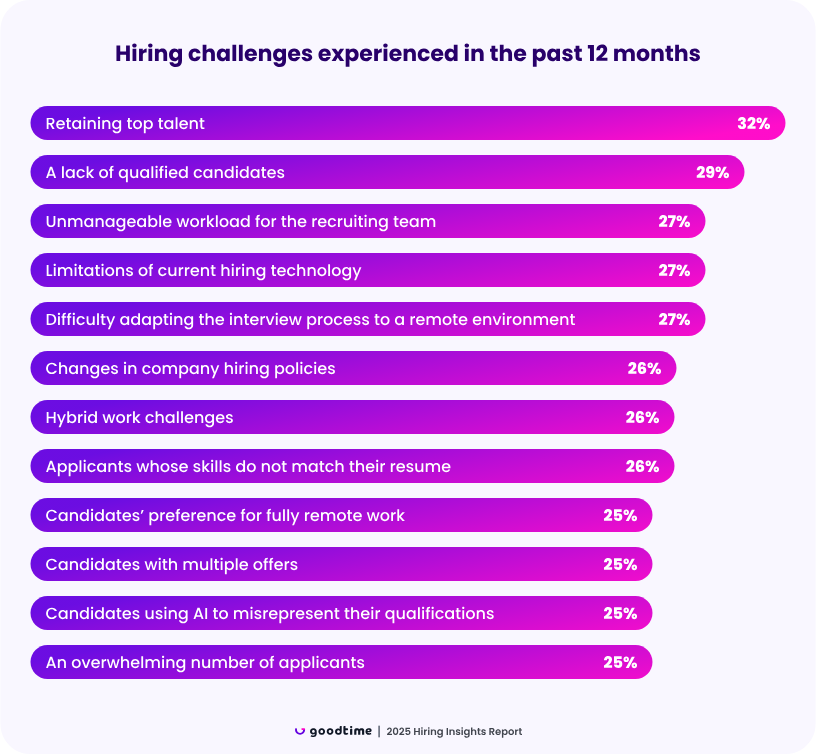
\includegraphics[width=1\linewidth]{img/hiring-challenges.png}
\caption{\centering\itshape Các thách thức trong tuyển dụng 12 tháng qua (Nguồn: GoodTime)}
\label{fig:hiring-challenges}
\end{figure}

Trong bối cảnh đó, ứng dụng trí tuệ nhân tạo (AI) và tự động hóa nổi lên như một hướng đi đột phá. Luận văn này tập trung nghiên cứu cách tiếp cận này nhằm giải quyết các thách thức của đội ngũ TA, đặc biệt là những hạn chế về công nghệ và sự kém hiệu quả của quy trình thủ công. Mục tiêu là khai thác tiềm năng của AI để tự động hóa các công việc lặp lại, từ đó giải phóng nguồn lực con người cho những nhiệm vụ chiến lược hơn — những nhiệm vụ vốn được các đội ngũ TA đánh giá là cấp thiết.

Thực tiễn cho thấy AI đang dần thay đổi cách các tổ chức xử lý những vấn đề cố hữu trong tuyển dụng. Các công nghệ tự động hóa đã và đang hỗ trợ đáng kể trong các công việc như lập lịch phỏng vấn, sàng lọc hồ sơ, và phân tích dữ liệu, giúp chuyên viên tuyển dụng có thêm thời gian tập trung vào các ưu tiên chiến lược như xây dựng mối quan hệ với ứng viên.

\begin{figure}[H]
\centering
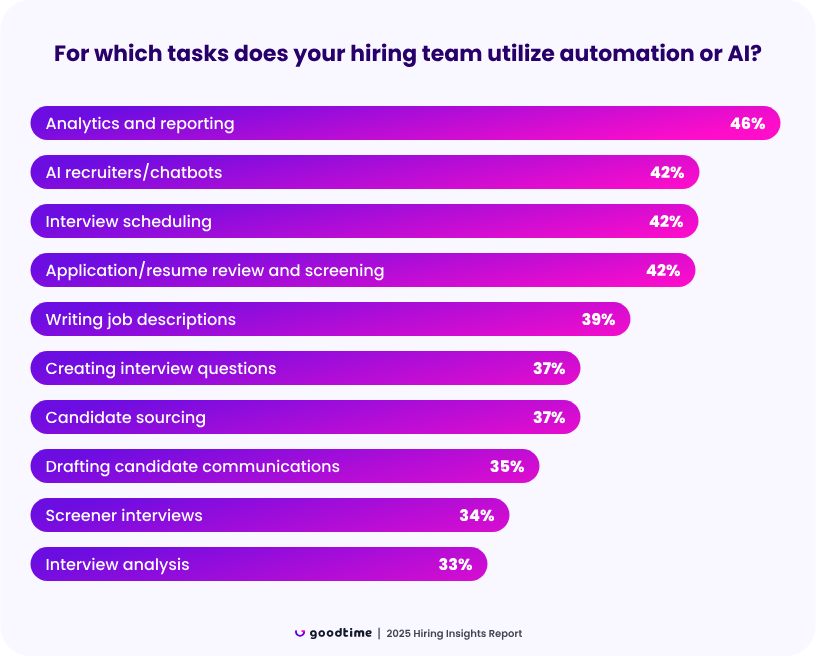
\includegraphics[width=1\linewidth]{img/hr-utilize-ai.png}
\caption{\centering\itshape Các nhiệm vụ trong tuyển dụng ứng dụng tự động hóa/AI (Nguồn: GoodTime)}
\label{fig:hr-utilize-ai}
\end{figure}

Sự dịch chuyển này không chỉ nâng cao hiệu suất mà còn đang định hình lại vai trò của chuyên viên tuyển dụng. Thay vì bị bó buộc vào công việc hành chính, họ dần trở thành những "cố vấn nhân tài" (talent advisor), tập trung vào chiến lược, phân tích và xây dựng quan hệ. Tương lai của ngành được dự báo sẽ chứng kiến sự phát triển mạnh mẽ của vai trò này.

Như bà Megan Hennessy, cựu Trưởng phòng Nhân tài Cấp cao Toàn cầu tại Meta, đã nhận định, vai trò của bộ phận thu hút nhân tài sẽ được nâng tầm một cách thực sự. Họ sẽ không còn chỉ là người tìm kiếm hay điều phối, mà sẽ trở thành những cố vấn chiến lược, định hướng cách thức và chiến lược tuyển dụng cho toàn tổ chức.

\begin{figure}[H]
\centering
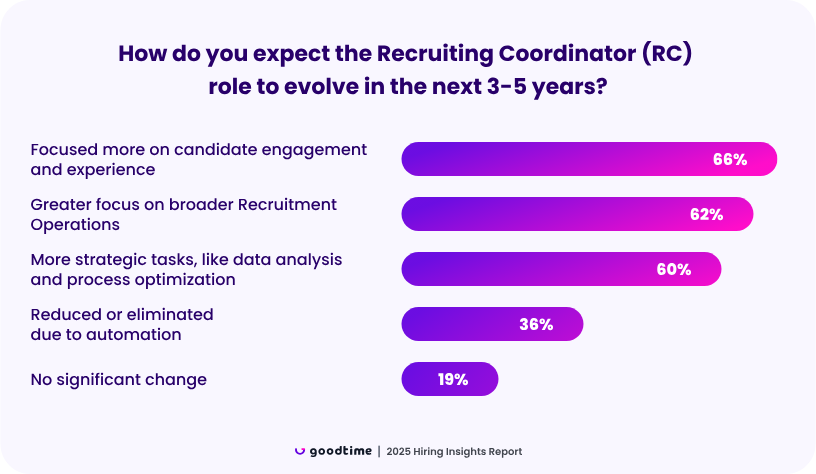
\includegraphics[width=1\linewidth]{hiring-evolve.png}
\caption{\centering\itshape Kỳ vọng về sự phát triển của vai trò điều phối viên tuyển dụng trong 3–5 năm tới (Nguồn: GoodTime)}
\label{fig:hiring-evolve}
\end{figure}

\subsection{Phạm vi bài toán}
Thị trường lao động hiện nay đang đối mặt với một nghịch lý: dù số lượng ứng viên dồi dào, các doanh nghiệp vẫn phải vật lộn để tìm kiếm nhân tài thực sự phù hợp, với thời gian tuyển dụng trung bình kéo dài đến 43 ngày. Thực trạng này bắt nguồn từ hai vấn đề cốt lõi và có liên quan mật thiết trong quy trình tuyển dụng truyền thống:

\begin{enumerate}[topsep=0pt, itemsep=0pt, leftmargin=40pt, label=\arabic*.]
    \item \textbf{Sự kém hiệu quả của quy trình thủ công}: Các tác vụ hành chính lặp lại, thiếu tự động hóa khiến quy trình tuyển dụng bị trì trệ, tăng chi phí và làm giảm khả năng cạnh tranh trong việc thu hút nhân tài.
    \item \textbf{Tỷ lệ loại sai cao và thất thoát nhân tài mang tính hệ thống}: Việc phụ thuộc quá mức vào các hệ thống ATS với những bộ lọc cứng nhắc đã loại bỏ một lượng lớn ứng viên tiềm năng một cách sai lầm.
\end{enumerate}

Mặc dù cả hai vấn đề đều quan trọng, luận văn này lập luận rằng việc giải quyết vấn đề thứ hai — giảm thiểu thất thoát nhân tài do hệ thống loại sai — mang đến cơ hội can thiệp cấp thiết và có tác động sâu sắc hơn. Một quy trình dù được tự động hóa hiệu quả (giải quyết vấn đề 1) cũng sẽ trở nên vô nghĩa nếu nó liên tục loại bỏ nhầm những ứng viên chất lượng (vấn đề 2). Do đó, việc khắc phục điểm yếu nền tảng này không chỉ khả thi hơn về mặt nghiên cứu nhờ có sẵn dữ liệu công khai và tiêu chí đánh giá cụ thể, mà còn hứa hẹn mang lại giá trị chiến lược rõ rệt cho chất lượng tuyển dụng tổng thể.

Vấn đề cốt lõi này xuất phát từ sự phụ thuộc nặng nề vào các hệ thống ATS, vốn được chứng minh là hoạt động kém hiệu quả khi loại sai từ 12\% đến 35\% ứng viên tiềm năng. Nguyên nhân chính là các bộ lọc dựa trên từ khóa cứng nhắc, dễ dàng bỏ qua những hồ sơ có năng lực cao nhưng "phi truyền thống", chẳng hạn như có khoảng trống nghề nghiệp hoặc thiếu bằng cấp hình thức. Tỷ lệ loại sai cao này không chỉ là một vấn đề kỹ thuật mà còn là một thất bại chiến lược, gây ra nhiều hệ quả tiêu cực:

\begin{itemize}[topsep=0pt, itemsep=0pt, leftmargin=40pt]
    \item \textbf{Thu hẹp nguồn ứng viên}: Nguồn nhân tài tiềm năng bị thu hẹp một cách giả tạo, làm trầm trọng thêm tình trạng thiếu hụt nhân sự.
    \item \textbf{Chi phí cơ hội cao}: Doanh nghiệp mất đi những ứng viên xuất sắc vào tay đối thủ cạnh tranh, gây thiệt hại về năng suất và đổi mới.
    \item \textbf{Tổn hại thương hiệu tuyển dụng}: Trải nghiệm ứng tuyển kém làm suy giảm hình ảnh của nhà tuyển dụng trong mắt ứng viên.
    \item \textbf{Duy trì định kiến}: Các bộ lọc cứng nhắc vô tình gây bất lợi cho một số nhóm nhân khẩu học, đi ngược lại các mục tiêu về đa dạng, bình đẳng và hòa nhập (DEI).
\end{itemize}

Vì vậy, luận văn này tập trung giải quyết vấn đề thất thoát nhân tài bằng cách đề xuất một hệ thống tuyển dụng thông minh, có sự tham gia của con người (human-in-the-loop), được thiết kế nhằm giảm tỷ lệ loại sai nhưng không làm tăng gánh nặng công việc cho chuyên viên. Cách tiếp cận này được hiện thực hóa thông qua một kiến trúc đa tác nhân (Multi-Agent System), nơi các tác nhân phần mềm chuyên biệt phối hợp linh hoạt với chuyên viên tuyển dụng để vừa tận dụng sức mạnh của tự động hóa, vừa duy trì sự tinh tế trong phán đoán của con người.

Từ đó, bài toán nghiên cứu của luận văn được phát biểu chính thức như sau:

\begin{itemize}[topsep=0pt, itemsep=0pt, leftmargin=40pt]
    \item \textbf{Đầu vào}: Một tập hợp các mô tả công việc $J$ và một tập hợp hồ sơ ứng viên $R$.
    \item \textbf{Nhiệm vụ}: Xử lý đầu vào để tạo ra một danh sách rút gọn được xếp hạng $S\subset R$ cho mỗi công việc $j\in J$, kèm theo giải thích rõ ràng, dễ hiểu cho thứ hạng của từng ứng viên.
    \item \textbf{Mục tiêu}: Tối đa hóa khả năng thu hồi các ứng viên thực sự đủ điều kiện (do chuyên viên xác nhận) mà các hệ thống ATS hiện tại bỏ sót, đồng thời giảm tải nhận thức cho chuyên viên thông qua các bản tóm tắt súc tích và chính xác.
\end{itemize}

\subsection{Trình bày bài toán}

Xuất phát từ thực trạng các hệ thống theo dõi ứng viên (ATS) và quy trình sàng lọc thủ công đang loại bỏ một tỷ lệ đáng kể ứng viên đủ điều kiện, dẫn đến chi phí tuyển dụng cao và làm suy giảm sự đa dạng của nguồn nhân lực, luận văn này đặt ra một câu hỏi nghiên cứu trọng tâm: Liệu một kiến trúc đa tác nhân có sự tham gia của con người (human-in-the-loop) có thể giảm thiểu Tỷ lệ Loại nhầm (False-Rejection Rate - FRR) mà không làm gia tăng gánh nặng đánh giá cho chuyên viên tuyển dụng hay không?.

Để hiện thực hóa mục tiêu trên, nghiên cứu sẽ tập trung vào việc thiết kế và kiểm nghiệm một hệ thống nguyên mẫu có khả năng:

\begin{enumerate}[topsep=0pt, itemsep=0pt, leftmargin=40pt, label=\arabic*.]
    \item \textbf{Tạo danh sách rút gọn với hiệu suất vượt trội}: Hệ thống phải có khả năng thu hồi (recall) ứng viên chất lượng cao hơn so với các hệ thống ATS tiêu chuẩn.
    \item \textbf{Tối ưu hóa khối lượng công việc}: Giảm số lượng hồ sơ mà chuyên viên cần xem xét xuống một tỷ lệ nhỏ trong tổng số ứng viên, được đo bằng chỉ số Giảm tải cho người đánh giá (Reviewer-Load-Reduction – RLR).
    \item \textbf{Đảm bảo tính minh bạch}: Cung cấp các giải thích rõ ràng và có thể kiểm chứng cho mọi đề xuất xếp hạng, giúp nhà tuyển dụng tin tưởng và ra quyết định nhanh chóng.
\end{enumerate}

Các tập dữ liệu hồ sơ công khai (1,000 hồ sơ đã gán nhãn) cùng với mô tả công việc thu thập từ web sẽ được sử dụng làm tập huấn luyện và kiểm tra.

Các kết quả kỳ vọng của luận văn bao gồm việc xây dựng một khuôn khổ kiến trúc đa tác nhân hoàn chỉnh (bao gồm các tác nhân Screening, Critic, Human-in-the-loop và Data-Steward) và cung cấp bằng chứng thực nghiệm về hiệu quả của nó trong việc cân bằng giữa giảm tỷ lệ loại sai (FRR) và khối lượng công việc của chuyên viên.

\newpage
\tocless\section{Cơ sở lý thuyết và công nghệ}
\setcounter{section}{2}
\addcontentsline{toc}{section}{\numberline{}CHƯƠNG 2: CƠ SỞ LÝ THUYẾT VÀ CÔNG NGHỆ}
\label{sec:chapter-2}

Chương này đặt nền móng lý thuyết và công nghệ cho toàn bộ luận văn. Nội dung được cấu trúc thành hai phần chính. 

Phần đầu tiên, Nền tảng Công nghệ, sẽ giới thiệu các khái niệm kỹ thuật cốt lõi làm nên giải pháp được đề xuất, bao gồm Mô hình Ngôn ngữ Lớn (LLM), Tác nhân AI (AI Agents), cơ chế sử dụng Công cụ (Tools), kiến trúc Hệ Đa tác nhân (Multi-Agent Systems – MAS), và vai trò của Con người trong Vòng lặp (Human-in-the-Loop – HITL).

Phần thứ hai, Cơ sở lý thuyết trong Quản trị Nguồn nhân lực, sẽ áp dụng các khái niệm công nghệ này vào bối cảnh cụ thể của bài toán tuyển dụng. Phần này sẽ phân tích ngắn gọn những thách thức trong hoạt động Thu hút nhân tài (Talent Acquisition), thiết lập cơ sở lý thuyết cho các tác nhân chuyên biệt được đề xuất, và định nghĩa khung đánh giá hiệu suất dựa trên các chỉ số học máy tiêu chuẩn.

Bằng cách kết hợp hai phần này, chương sẽ xây dựng một luận cứ chặt chẽ, kết nối công nghệ nền tảng với ứng dụng thực tiễn và phương pháp đo lường, tạo ra một cơ sở vững chắc cho việc thiết kế và kiểm nghiệm mô hình trong các chương tiếp theo.

\vspace{14pt}

\setcounter{subsection}{0}
\setcounter{table}{0}
\setcounter{figure}{0}
\subsection{Nền tảng công nghệ}

\subsubsection{Mô hình Ngôn ngữ Lớn (Large Language Models – LLM)}

Mô hình Ngôn ngữ Lớn (Large Language Model - LLM) là một loại chương trình trí tuệ nhân tạo (AI) được thiết kế để nhận diện, hiểu và tạo ra văn bản ngôn ngữ tự nhiên của con người. Huấn luyện trên bộ dữ liệu văn bản khổng lồ, các mô hình này học các mẫu hình về cú pháp, ngữ nghĩa, kiến thức thực tiễn và các mối quan hệ khái niệm giữa các từ.

Kiến trúc nền tảng cho phần lớn các LLM hiện đại là Transformer, một kiến trúc sử dụng cơ chế tự chú ý (self-attention mechanism) để xử lý song song các từ trong câu, giúp mô hình hiểu được các mối quan hệ phức tạp, kể cả những phụ thuộc dài trong văn bản. Nhờ đó, LLM có khả năng thực hiện nhiều tác vụ ấn tượng như sinh văn bản, tóm tắt, dịch thuật và trả lời câu hỏi với tính mạch lạc và phù hợp ngữ cảnh cao.

Quy trình xử lý của một Mô hình Ngôn ngữ Lớn bao gồm bốn bước chính:

\begin{itemize}[topsep=0pt, itemsep=0pt, leftmargin=40pt]
    \item \textbf{Tokenization}: Văn bản đầu vào được chia nhỏ thành các đơn vị nhỏ hơn (tokens) để xử lý.
    \item \textbf{Training on Large Datasets}: Mô hình được huấn luyện trên các tập dữ liệu văn bản khổng lồ để học cách hiểu ngôn ngữ.
    \item \textbf{Attention Mechanisms}: Mô hình đánh giá tầm quan trọng của từng từ trong ngữ cảnh chung, nhờ cơ chế tự chú ý.
    \item \textbf{Text Generation}: Mô hình tạo ra văn bản đầu ra, đảm bảo mạch lạc và phù hợp với ngữ cảnh.
\end{itemize}

Hình ảnh cũng cho thấy quá trình này diễn ra như một con đường tuần tự nhưng linh hoạt, phản ánh cách LLM xử lý và tạo ra văn bản một cách hiệu quả và có hệ thống.

\paragraph{Tokenization}

Tokenization là bước tiền xử lý quan trọng trong các mô hình ngôn ngữ lớn, nhằm chia văn bản đầu vào thành các đơn vị nhỏ hơn gọi là tokens. Các token này có thể là ký tự, từ, hoặc thậm chí là từng phần của từ, tùy thuộc vào phương pháp mã hóa được sử dụng (ví dụ: Byte-Pair Encoding, WordPiece, SentencePiece). Việc chuyển văn bản sang dạng chuỗi token giúp mô hình xử lý văn bản hiệu quả hơn và học được các quy luật thống kê của ngôn ngữ. Tokenization còn giúp mô hình có thể xử lý cả những từ chưa từng thấy (out-of-vocabulary) bằng cách tách chúng thành các token con (subword tokens).

\begin{figure}[H]
    \centering
    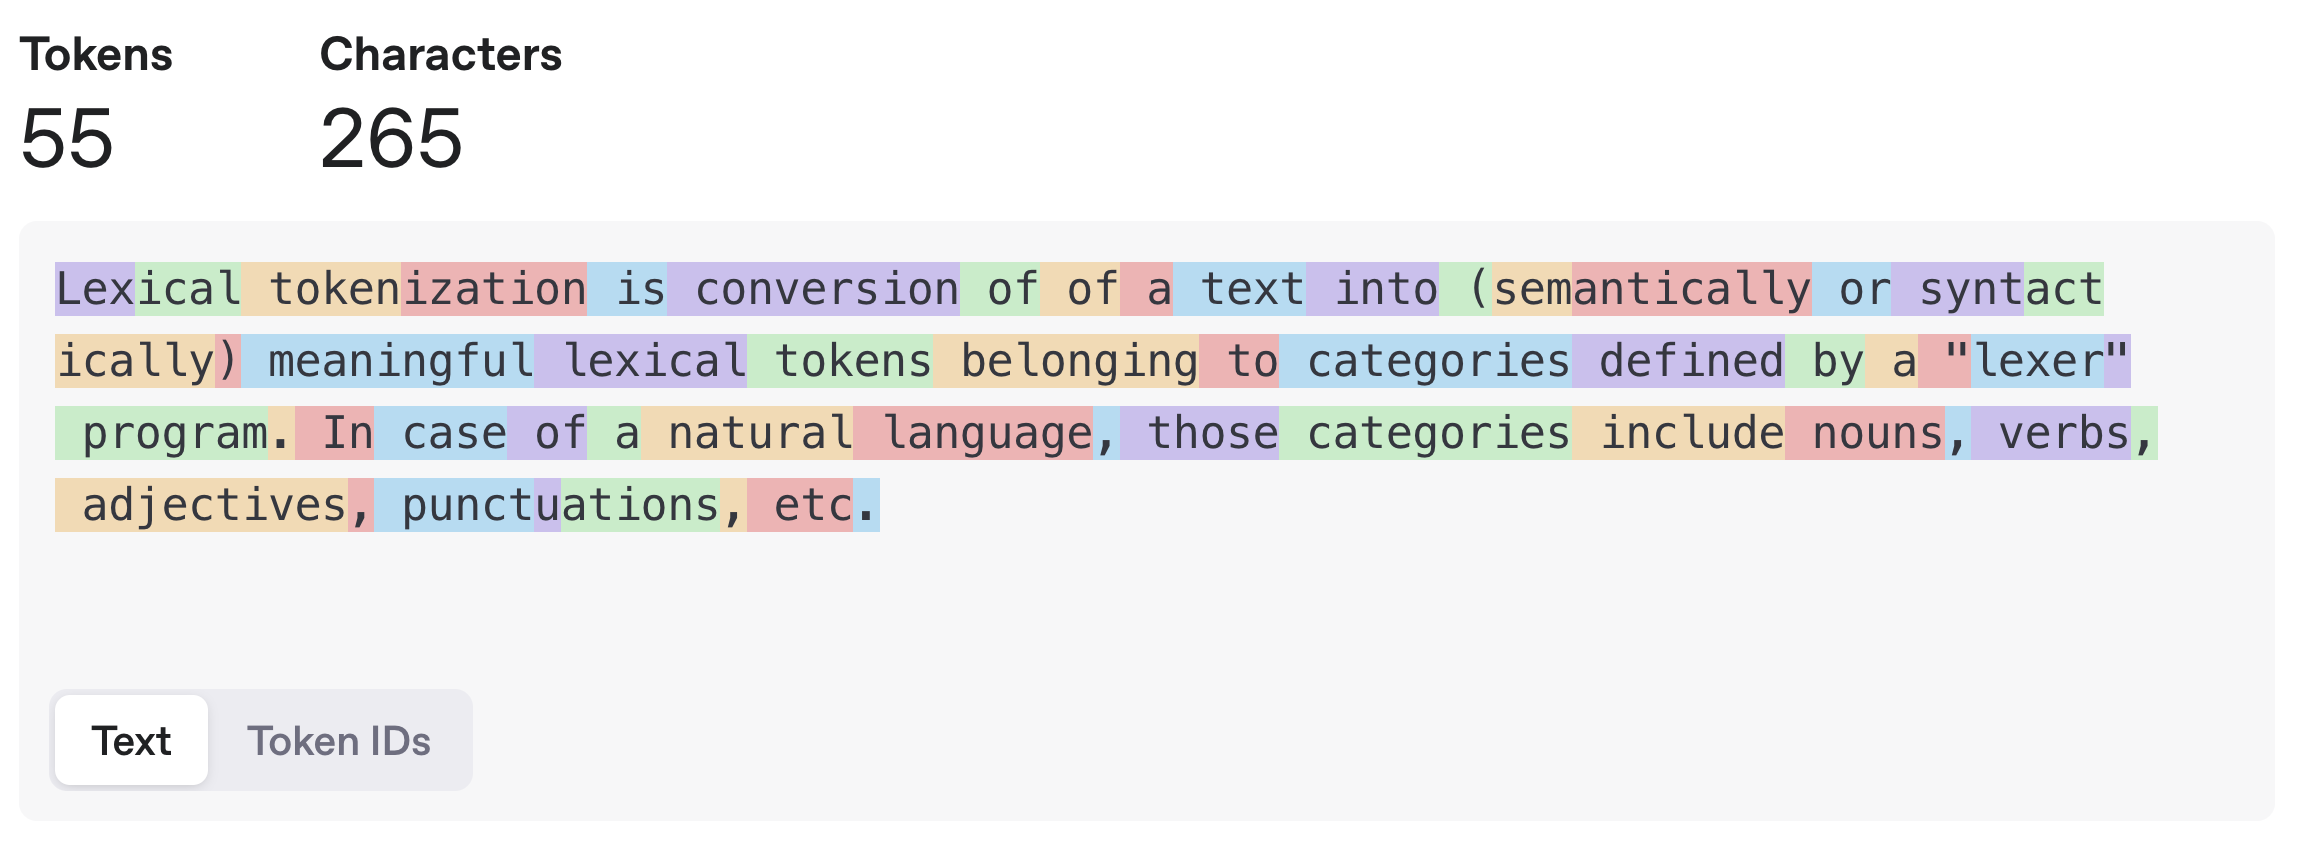
\includegraphics[width=1\linewidth]{img/llm-tokenizers.png}
    \caption{\textit{Công cụ Tokenizer của OpenAI}}
    \label{fig:2.1.2}
\end{figure}

\paragraph{Bộ dữ liệu của LLM (LLM's Dataset)}

Một yếu tố quan trọng quyết định chất lượng của LLM chính là bộ dữ liệu huấn luyện. Các mô hình này được huấn luyện trên tập hợp văn bản khổng lồ, bao gồm dữ liệu từ web, sách, báo, Wikipedia và nhiều nguồn chuyên ngành khác. Quy mô và đa dạng của dữ liệu giúp mô hình học được các mẫu ngôn ngữ phổ quát, kiến thức nền và các sắc thái ngữ nghĩa tinh vi. Tuy nhiên, điều này cũng đặt ra những thách thức về tính đại diện, thiên lệch (bias) và chất lượng dữ liệu, đòi hỏi các bước tiền xử lý cẩn thận nhằm đảm bảo mô hình không chỉ chính xác mà còn công bằng và đáng tin cậy.

\hyperref[fig:distribution-data-in-c4-dataset]{\textcolor{blue}{Hình 2.3}} minh họa tỷ lệ phân bố các lĩnh vực nội dung trong tập dữ liệu C4 (\href{https://arxiv.org/abs/1910.10683}{Colossal Clean Crawled Corpus}) — một tập dữ liệu văn bản quy mô lớn, thường được sử dụng để huấn luyện các mô hình ngôn ngữ lớn (LLM). C4 được Google giới thiệu, là phiên bản đã được làm sạch và lọc của tập dữ liệu \href{https://commoncrawl.org/}{Common Crawl}, nhằm loại bỏ nội dung kém chất lượng và đảm bảo tính đa dạng, phù hợp cho các bài toán xử lý ngôn ngữ tự nhiên.

\begin{figure}[H]
    \centering
    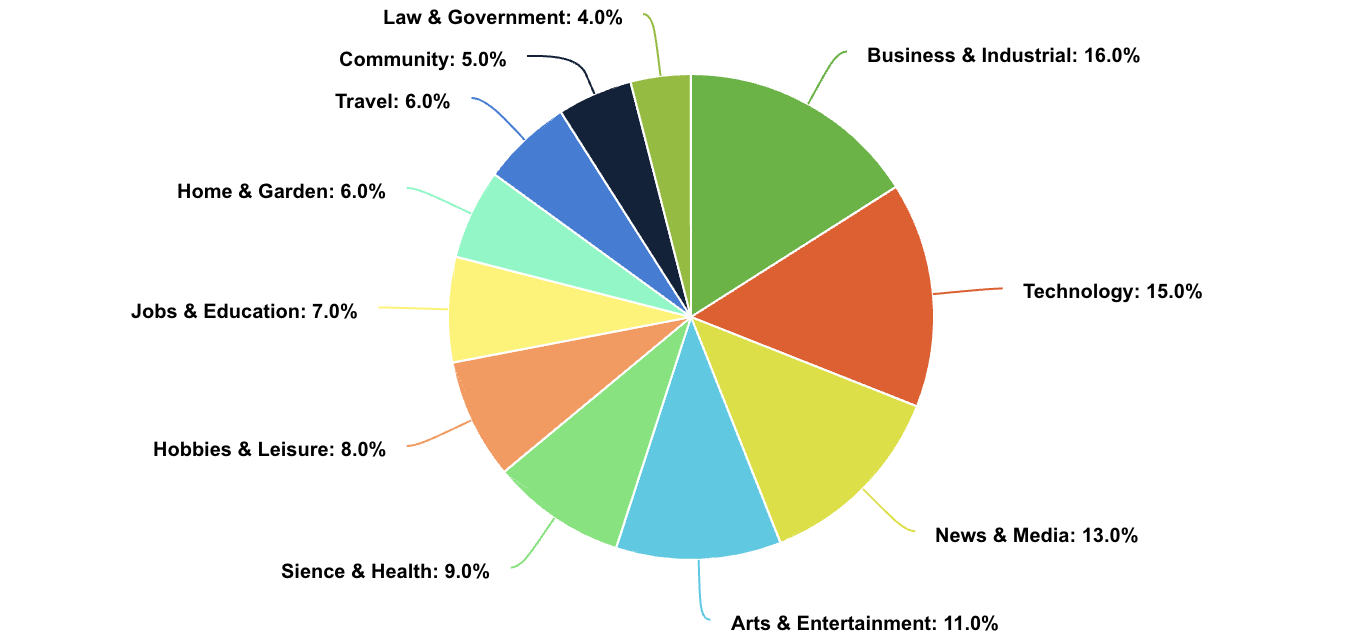
\includegraphics[width=1\linewidth]{img/distribution-data-in-c4-dataset.png}
    \caption{\centering\textit{Phân bố các lĩnh vực trong tập dữ liệu C4}}
    \label{fig:distribution-data-in-c4-dataset}
\end{figure}

\paragraph{Kiến trúc Transformer (Transformer Architecture)}

Transformer là kiến trúc nền tảng đằng sau phần lớn các LLM hiện đại. Được giới thiệu lần đầu tiên trong bài báo Attention Is All You Need, Transformer mang đến bước đột phá nhờ khả năng xử lý song song và cơ chế tự chú ý (self-attention), vượt trội so với các mạng hồi tiếp (RNN, LSTM) truyền thống. Mỗi Transformer gồm hai thành phần chính: encoder và decoder, trong đó LLM thường sử dụng cấu trúc decoder-only hoặc encoder-decoder tùy bài toán.

Cơ chế tự chú ý cho phép mô hình xác định tầm quan trọng tương đối của từng token trong ngữ cảnh, bằng cách tính toán ma trận trọng số giữa các token. 

\begin{figure}[H]
    \centering
    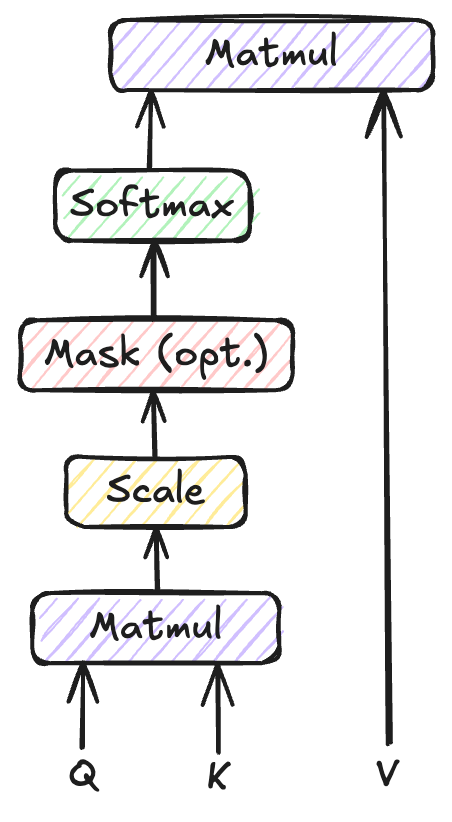
\includegraphics[width=0.2\linewidth]{img/transformer-architecture.png}
    \caption{\textit{Kiến trúc Transformer}}
    \label{2.1.4}
\end{figure}

Với đầu vào là một tập hợp $n$ token được biểu diễn dưới dạng embedding $X\in \mathbb{R}^{n\times d}$, ta tính ba ma trận:
\begin{gather*}
Q = XW_Q,\ K = XW_K,\ V=XW_V
\end{gather*}
trong đó $W_Q$, $W_K$, $W_V$ là các trọng số học được. Trọng số chú ý được tính bằng công thức:
\begin{gather*}
    \text{Attention}(Q,K,V) = \text{softmax}\left(\frac{QK^T}{\sqrt{d_k}}\right)V
\end{gather*}
với $d_k$ là kích thước của vector khóa. Kết quả này cho phép mô hình gán mức quan trọng khác nhau cho các token, từ đó học được các phụ thuộc dài hạn và ngữ cảnh sâu sắc hơn.

Ngoài self-attention, Transformer còn sử dụng các kỹ thuật như \textit{positional encoding} để mô hình có thể hiểu thứ tự của các token, cùng với các lớp feed-forward, normalization và residual connections giúp huấn luyện ổn định và hiệu quả. Chính nhờ sự kết hợp này mà Transformer đã trở thành xương sống của các LLM hiện đại, từ GPT đến BERT và các biến thể khác.

\subsubsection{Tác nhân AI (AI Agent)}

Tác nhân AI (AI Agent) là một thực thể phần mềm có khả năng tự động ra quyết định và thực hiện hành động nhằm đạt được các mục tiêu đã định, dựa trên việc quan sát môi trường, suy luận và học hỏi. Trong bối cảnh quản lý nhân sự (HRM), tác nhân AI đóng vai trò quan trọng trong việc hỗ trợ hoặc tự động hóa các quy trình, từ tìm kiếm ứng viên, lên lịch phỏng vấn, đến quản lý hiệu suất và đề xuất đào tạo.

Ngày nay, với sự phát triển của LLMs, một xu hướng phổ biến là thiết kế các tác nhân AI với \textit{bộ não} là LLM. LLM đóng vai trò như một trung tâm suy luận và lập kế hoạch, giúp tác nhân không chỉ thực hiện các hành động theo quy tắc cứng nhắc mà còn có khả năng hiểu ngữ cảnh, lập kế hoạch nhiều bước, và thích ứng với các tình huống mới. Ví dụ, trong một hệ thống tuyển dụng, LLM có thể giúp tác nhân phân tích CV, soạn email phỏng vấn phù hợp, hoặc trả lời câu hỏi của ứng viên một cách tự nhiên và cá nhân hóa.

\paragraph{Kiến trúc tổng quan}
\begin{figure}[H]
    \centering
    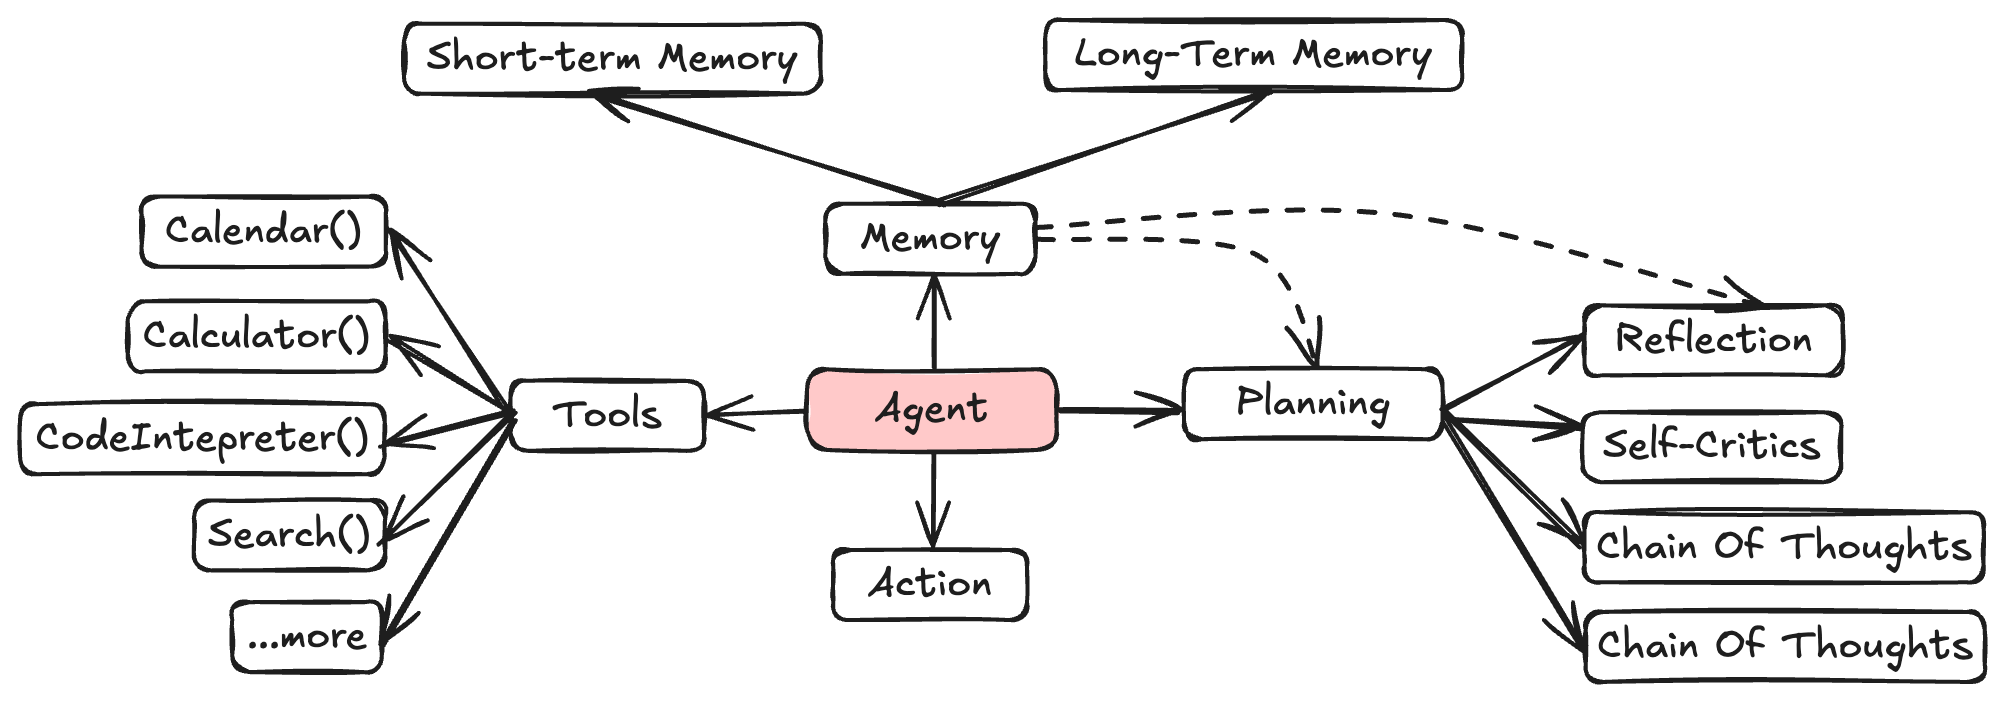
\includegraphics[width=1\linewidth]{img/ai-agent-architecture.png}
    \caption{\centering\textit{Kiến trúc tổng quan của một tác nhân AI}}
    \label{fig:2.1.5}
\end{figure}
Một tác nhân AI hiện đại, điển hình là tác nhân dựa trên LLM, thường được cấu thành từ các thành phần chính sau:

\begin{itemize}[topsep=0pt, itemsep=0pt, leftmargin=40pt]
	\item \textbf{Memory (Bộ nhớ):} Gồm \textit{short-term memory} (bộ nhớ ngắn hạn) và \textit{long-term memory} (bộ nhớ dài hạn), giúp lưu trữ bối cảnh, dữ kiện và kinh nghiệm để phục vụ cho các quyết định và kế hoạch sau này.
	\item \textbf{Planning (Lập kế hoạch):} Bộ phận sử dụng sức mạnh của LLM để xây dựng chuỗi hành động, bao gồm các cơ chế như \textit{Reflection} (phản tư), \textit{Self-Critics} (tự đánh giá) và \textit{Chain of Thoughts} (chuỗi suy nghĩ).
	\item \textbf{Tools (Công cụ):} Các API hay chức năng chuyên biệt mà tác nhân có thể gọi, chẳng hạn như \texttt{Calendar()}, \texttt{Calculator()}, \texttt{CodeInterpreter()}, \texttt{Search()} và nhiều công cụ khác.
	\item \textbf{Action (Hành động):} Lớp này thực thi các quyết định hoặc kế hoạch, ví dụ như thao tác dữ liệu, truy xuất thông tin hoặc giao tiếp với môi trường bên ngoài.
\end{itemize}

\paragraph{LLM – Bộ não của tác nhân}
Các mô hình LLM như GPT-4, Claude, Gemini, hay LLaMA có khả năng suy luận theo ngữ cảnh, lên kế hoạch đa bước và tổng hợp thông tin từ nhiều nguồn. Trong vai trò là “bộ não” của tác nhân, LLM tiếp nhận yêu cầu và bối cảnh, quyết định các hành động tiếp theo và điều phối các công cụ để đạt mục tiêu. Một điểm quan trọng là LLM không trực tiếp thao tác với thế giới mà thông qua các \textit{tools}.

Lý do chính lựa chọn LLM làm bộ não của tác nhân là nhờ khả năng tự phản biện (self-reflection) và lập luận trên chính các phản hồi trước đó của mình. Sau khi tạo ra một phản hồi hoặc thực hiện một hành động, LLM có thể tự đánh giá xem kết quả đó có hợp lý, chính xác và phù hợp với mục tiêu hay không. Dựa trên đánh giá đó, LLM có thể tự động xây dựng một cách tiếp cận cụ thể hơn hoặc sửa đổi kế hoạch hành động để tiến gần hơn đến kết quả mong đợi. Khả năng này khiến LLM trở thành trung tâm suy luận linh hoạt và thích ứng, vượt trội so với các thuật toán ra quyết định cứng nhắc truyền thống.

\paragraph{Công cụ (Tools) và hành động}
Các tác nhân AI hiện đại có khả năng sử dụng nhiều công cụ được lập trình sẵn để thực thi các hành động cụ thể. Ví dụ:
\begin{itemize}[topsep=0pt, itemsep=0pt, leftmargin=40pt]
    \item Công cụ tìm kiếm: tra cứu thông tin mới.
    \item Công cụ cơ sở dữ liệu: truy vấn hoặc cập nhật hồ sơ ứng viên.
    \item Công cụ lập lịch: kết nối với lịch tổ chức để lên lịch họp/phỏng vấn.
    \item Công cụ giao tiếp: gửi email, tin nhắn, hoặc trả lời chatbot.
\end{itemize}

Cơ chế này được gọi là \textit{Tool-augmented Agent}, nơi tác nhân sử dụng LLM để xác định khi nào và công cụ nào cần được sử dụng, sau đó ra lệnh thực hiện.

\paragraph{Chu trình hoạt động của tác nhân}
Quá trình làm việc của một tác nhân hiện đại dựa trên LLM không chỉ đơn thuần là quan sát – hành động – phản hồi mà còn bao gồm các cơ chế lập luận, tự phản biện và điều chỉnh liên tục. \hyperref[fig:agent-workflow]{\textcolor{blue}{Hình 2.5}} minh họa rõ nét các bước trong chu trình này.

\begin{figure}[H]
    \centering
    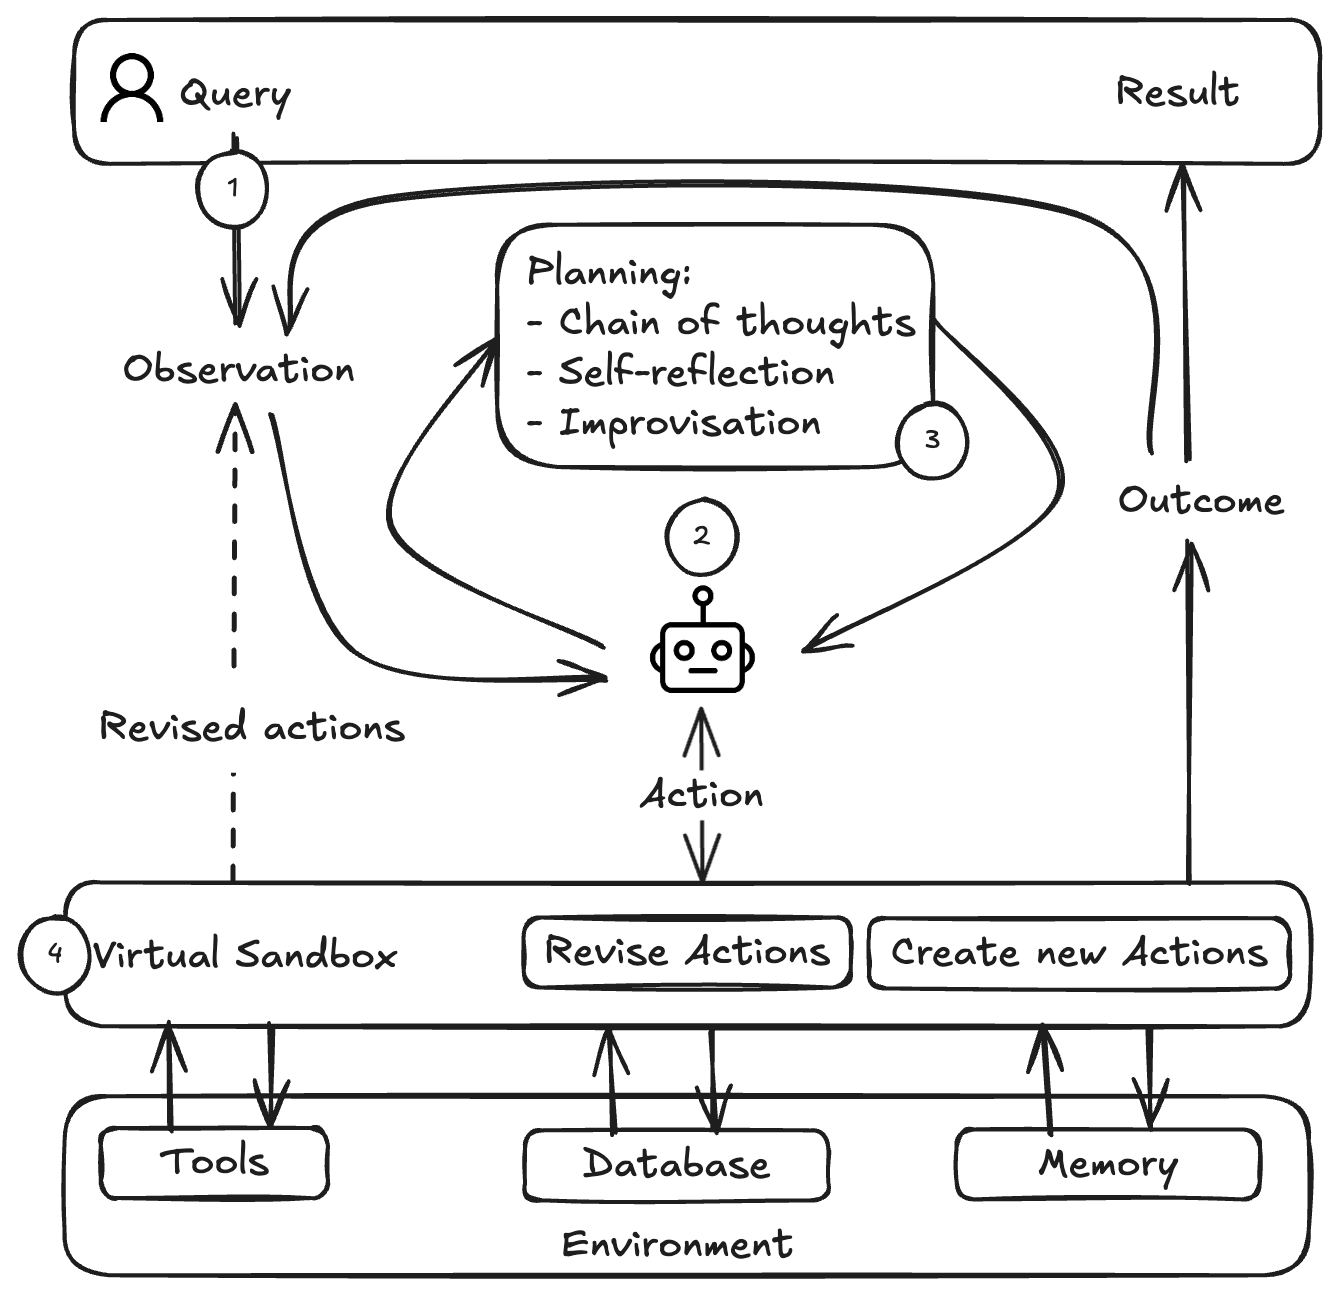
\includegraphics[width=0.8\linewidth]{img/agent-workflow.png}
    \caption{\centering \textit{Cách thức hoạt động của tác nhân AI}}
    \label{fig:agent-workflow}
\end{figure}

\begin{enumerate}[topsep=0pt, itemsep=2pt, leftmargin=40pt, label=\arabic*.]
    \item \textbf{Observation (Quan sát):} Khi người dùng gửi một yêu cầu (query), tác nhân trước hết sẽ quan sát môi trường, bao gồm dữ liệu hiện có, trạng thái hệ thống, thông tin từ bộ nhớ, và đầu vào của người dùng.
    \item \textbf{Planning (Lập kế hoạch):} Dựa trên quan sát, tác nhân kích hoạt “bộ não” LLM để lập kế hoạch hành động. Quá trình này sử dụng các kỹ thuật như \textit{Chain-of-Thought} để suy nghĩ theo từng bước, \textit{Self-reflection} để tự đánh giá tính hợp lý của kế hoạch, và \textit{Improvisation} để điều chỉnh khi gặp tình huống chưa lường trước.
    \item \textbf{Action (Thực thi):} Sau khi có kế hoạch cụ thể, tác nhân thực thi các hành động ban đầu bằng cách gọi các công cụ phù hợp (ví dụ: API, cơ sở dữ liệu, hệ thống email, chatbot). Các công cụ này chính là “cánh tay” giúp tác nhân tương tác với môi trường.
    \item \textbf{Calling tools (Gọi công cụ):} Trong quá trình thực hiện, tác nhân có thể cần truy xuất dữ liệu, cập nhật hồ sơ, gửi thông báo, hay gọi thêm các dịch vụ chuyên biệt. Tác nhân sử dụng một tập hợp các công cụ được định nghĩa sẵn, phối hợp với bộ nhớ và cơ sở dữ liệu để tạo ra hoặc điều chỉnh các hành động.
    \item \textbf{Outcome (Kết quả):} Sau khi thực hiện hành động, hệ thống trả lại kết quả cho người dùng. Nếu phát hiện kết quả chưa tối ưu hoặc sai lệch so với mục tiêu, tác nhân sẽ quay lại bước lập kế hoạch để điều chỉnh hành động (revised actions) trước khi hoàn tất.
\end{enumerate}


Chu trình khép kín này giúp tác nhân không chỉ phản ứng tức thời mà còn có khả năng tự điều chỉnh, học hỏi và cải thiện liên tục trong quá trình tương tác, đảm bảo tính chính xác và hiệu quả cao hơn trong các ứng dụng quản lý nhân sự.

\subsubsection{Hệ Đa tác nhân (Multi-Agent Systems – MAS)}

Hệ thống đa tác nhân (MAS) là một tập hợp các tác nhân phần mềm tự chủ, cùng tồn tại và tương tác trong một môi trường chung, nhằm đạt được các mục tiêu riêng biệt hoặc chung thông qua phối hợp. Mỗi tác nhân trong MAS có khả năng quan sát môi trường, ra quyết định độc lập, giao tiếp và hợp tác với các tác nhân khác. MAS được xem là một mô hình mạnh mẽ để giải quyết các vấn đề phân tán, phức tạp và đòi hỏi nhiều thành phần phối hợp.

Trong bối cảnh quản lý nhân sự, MAS mở ra cách tiếp cận mới để tự động hóa các quy trình phân tán như tuyển dụng, đánh giá hiệu suất, hoặc quản lý đào tạo, nơi nhiều tác nhân đại diện cho các bộ phận, nhân viên, hoặc hệ thống khác nhau. Khác với tác nhân đơn, MAS cho phép các tác nhân cùng làm việc, đàm phán hoặc phân chia nhiệm vụ, giúp tối ưu hóa hiệu quả toàn hệ thống và thích ứng linh hoạt với sự thay đổi của môi trường quản trị nhân sự.

\paragraph{Các thành phần chính của hệ thống đa tác nhân}
Một hệ thống đa tác nhân (MAS) được cấu thành từ bốn thành phần cốt lõi: tác nhân, môi trường, cơ chế giao tiếp và cơ chế phối hợp. Mỗi thành phần đóng vai trò riêng trong việc đảm bảo hệ thống vận hành hiệu quả và đạt được các mục tiêu đã định.

\begin{itemize}[topsep=0pt, itemsep=2pt, leftmargin=40pt]
    \item \textbf{Tác nhân (Agents)}: là đơn vị cơ bản trong MAS, đại diện cho một thực thể phần mềm tự chủ, có khả năng quan sát, ra quyết định và thực hiện hành động. Các tác nhân có thể được phân loại từ đơn giản đến phức tạp.
    \begin{itemize}
        \item \textbf{Tác nhân thụ động (passive agents)}: chỉ phản hồi trực tiếp với các kích thích từ môi trường, không có khả năng lập
        kế hoạch.
        \item \textbf{Tác nhân chủ động (active agents)}: có thể ra quyết định và thực hiện hành động nhằm đạt mục tiêu cụ thể, dựa trên trạng thái nội bộ và môi trường.
        \item \textbf{Tác nhân nhận thức (cognitive agents)}: sử dụng suy luận, lập kế hoạch nhiều bước, và thích nghi với những thay đổi để tối ưu hóa kết quả.
    \end{itemize}
    \item \textbf{Môi trường (Environment)}: là không gian mà các tác nhân tồn tại và tương tác. Đây có thể là một hệ thống ảo mô phỏng, một cơ sở dữ liệu phân tán hoặc hệ thống thực tế. Môi trường có thể được phân loại thành:
    \begin{itemize}
        \item \textbf{Môi trường ảo (virtual)}: tồn tại hoàn toàn trong không gian số, ví dụ như hệ thống thông tin HRM.
        \item \textbf{Môi trường rời rạc (discrete)}: không gian có tập hợp hữu hạn các trạng thái rõ ràng, ví dụ như quy trình phỏng vấn với các bước cố định.
        \item \textbf{Môi trường liên tục (continuous)}: không gian có vô số trạng thái, yêu cầu các tác nhân xử lý dữ liệu và ra quyết định một cách tinh vi hơn.
    \end{itemize}
    \item \textbf{Cơ chế giao tiếp (Communication)}: Để phối hợp, các tác nhân cần trao đổi thông tin thông qua các cơ chế giao tiếp. Việc giao tiếp thường dựa trên các giao thức chuẩn (như ACL – Agent Communication Language) và các từ điển khái niệm chung (ontology) để đảm bảo hiểu đúng ý nghĩa. Hình thức giao tiếp có thể là trực tiếp (gửi tin nhắn) hoặc gián tiếp (chia sẻ trạng thái môi trường).
    \item \textbf{Cơ chế phối hợp (Coordination and Cooperation)}: để đạt được mục tiêu chung hoặc tối ưu hóa hiệu suất tổng thể, các tác nhân cần phối hợp. Phối hợp có thể ở mức cơ bản, như phân chia nhiệm vụ, hoặc phức tạp, như đàm phán để giải quyết xung đột lợi ích. Các cơ chế phối hợp phổ biến gồm có dựa trên hợp đồng, đàm phán hoặc đồng thuận.
\end{itemize}

Trong thực tế, các hệ thống MAS thường sử dụng hỗn hợp nhiều loại tác nhân, tùy thuộc vào yêu cầu của bài toán. Tuy nhiên, phổ biến nhất là các tác nhân chủ động và nhận thức, vì chúng có khả năng tự lập kế hoạch, phối hợp và thích ứng — những đặc tính thiết yếu trong các môi trường phức tạp và phân tán như quản lý nhân sự.

\begin{figure}[H]
    \centering
    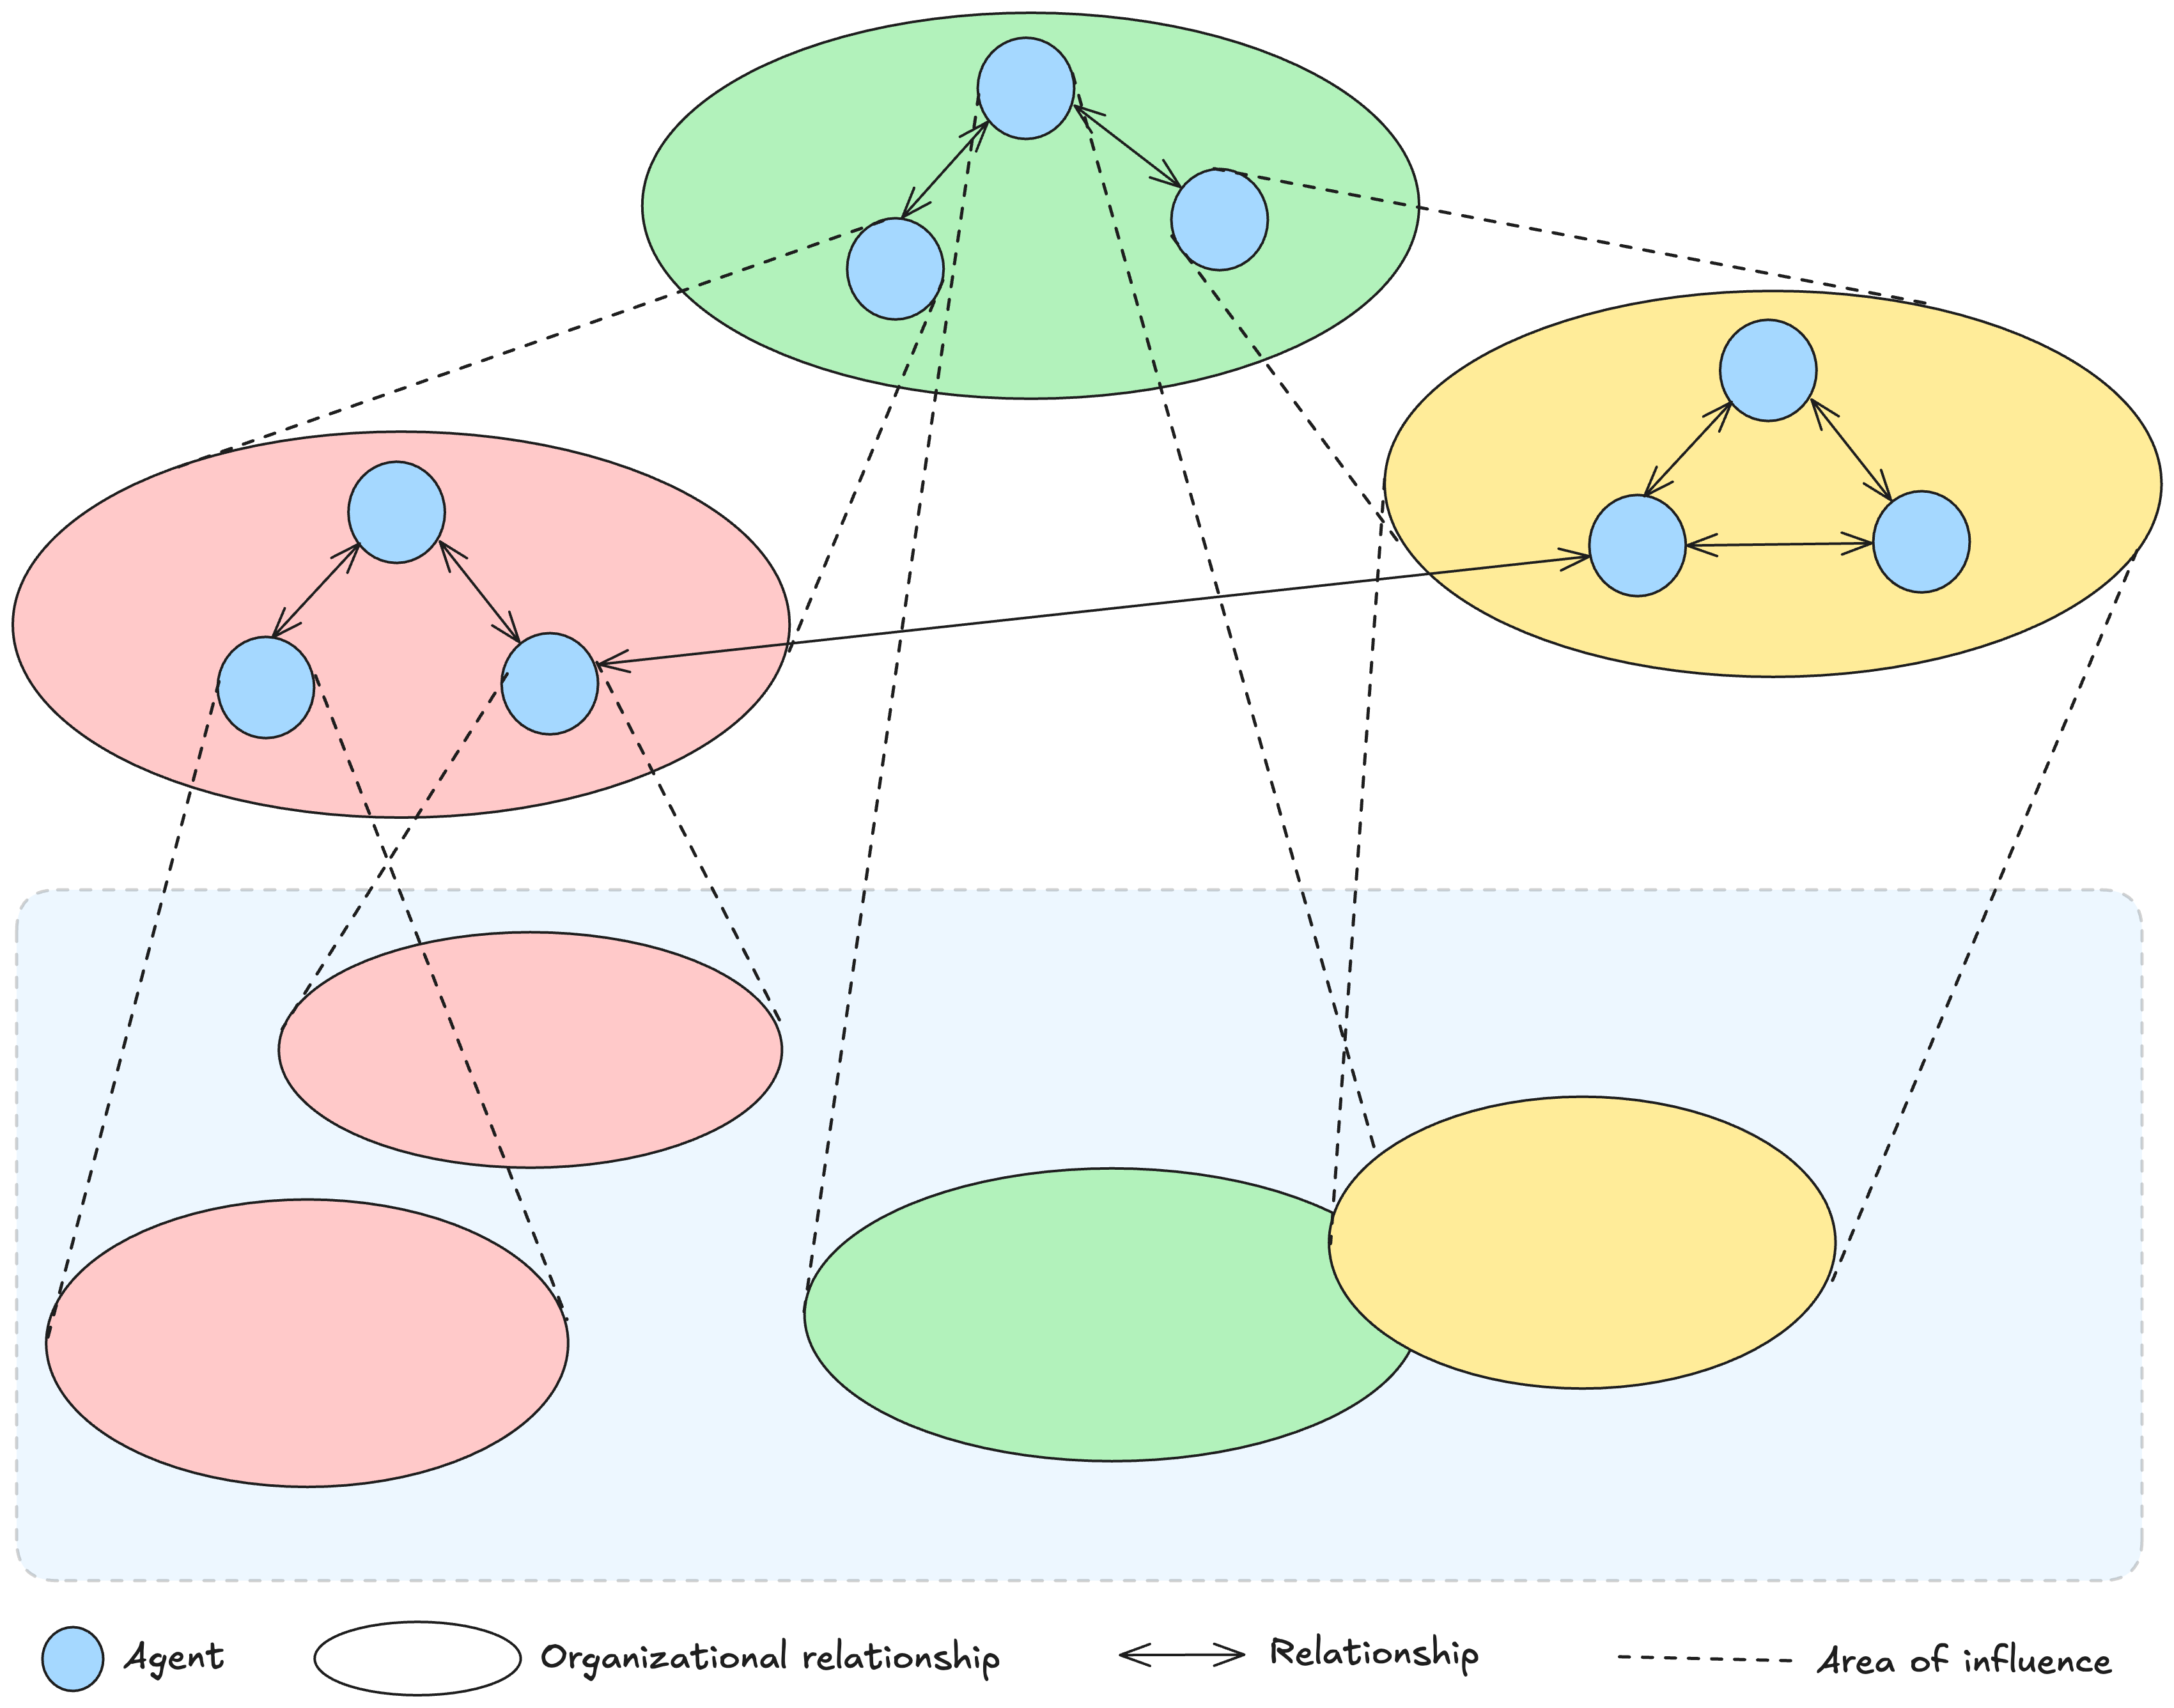
\includegraphics[width=1\linewidth]{img/mas.png}
    \caption{\centering \textit{Kiến trúc tổng quan của hệ thống đa tác nhân}}
    \label{fig:mas}
\end{figure}

\paragraph{Đặc điểm của hệ thống đa tác nhân}

Hệ thống đa tác nhân sở hữu một số đặc điểm nổi bật, giúp nó trở thành lựa chọn phù hợp cho các bài toán phân tán, phức tạp và có tính động cao:
\begin{itemize}[topsep=0pt, itemsep=2pt, leftmargin=40pt]
    \item \textbf{Tính phân tán (Distributedness)}: MAS được thiết kế để hoạt động trong môi trường phân tán, nơi các tác nhân có thể chạy trên các nền tảng hoặc địa điểm khác nhau nhưng vẫn phối hợp thông qua giao tiếp. Điều này giúp hệ thống mở rộng linh hoạt mà không bị phụ thuộc vào một điểm trung tâm.
    \item \textbf{Tính tự chủ (Autonomy)}: Mỗi tác nhân trong MAS có khả năng ra quyết định và thực hiện hành động độc lập dựa trên mục tiêu và trạng thái của chính nó, mà không cần sự điều khiển trực tiếp từ con người hoặc hệ thống trung tâm.
    \item \textbf{Tính xã hội (Social ability)}: Các tác nhân có khả năng giao tiếp và hợp tác với nhau để đạt được mục tiêu chung, hoặc đàm phán để tối ưu hóa mục tiêu riêng trong bối cảnh chung của hệ thống.
    \item \textbf{Tính thích nghi (Adaptivity)}: MAS có thể phản ứng và điều chỉnh hành vi khi môi trường hoặc yêu cầu thay đổi, nhờ khả năng tự tổ chức và học hỏi của các tác nhân.
    \item \textbf{Tính mở (Openness)}: Hệ thống MAS có khả năng mở rộng hoặc thu hẹp quy mô bằng cách thêm hoặc loại bỏ tác nhân mà không cần tái cấu trúc toàn bộ hệ thống. Tính mở giúp hệ thống duy trì hoạt động ổn định ngay cả khi cấu hình thay đổi.
\end{itemize}

\begin{figure}[H]
    \centering
    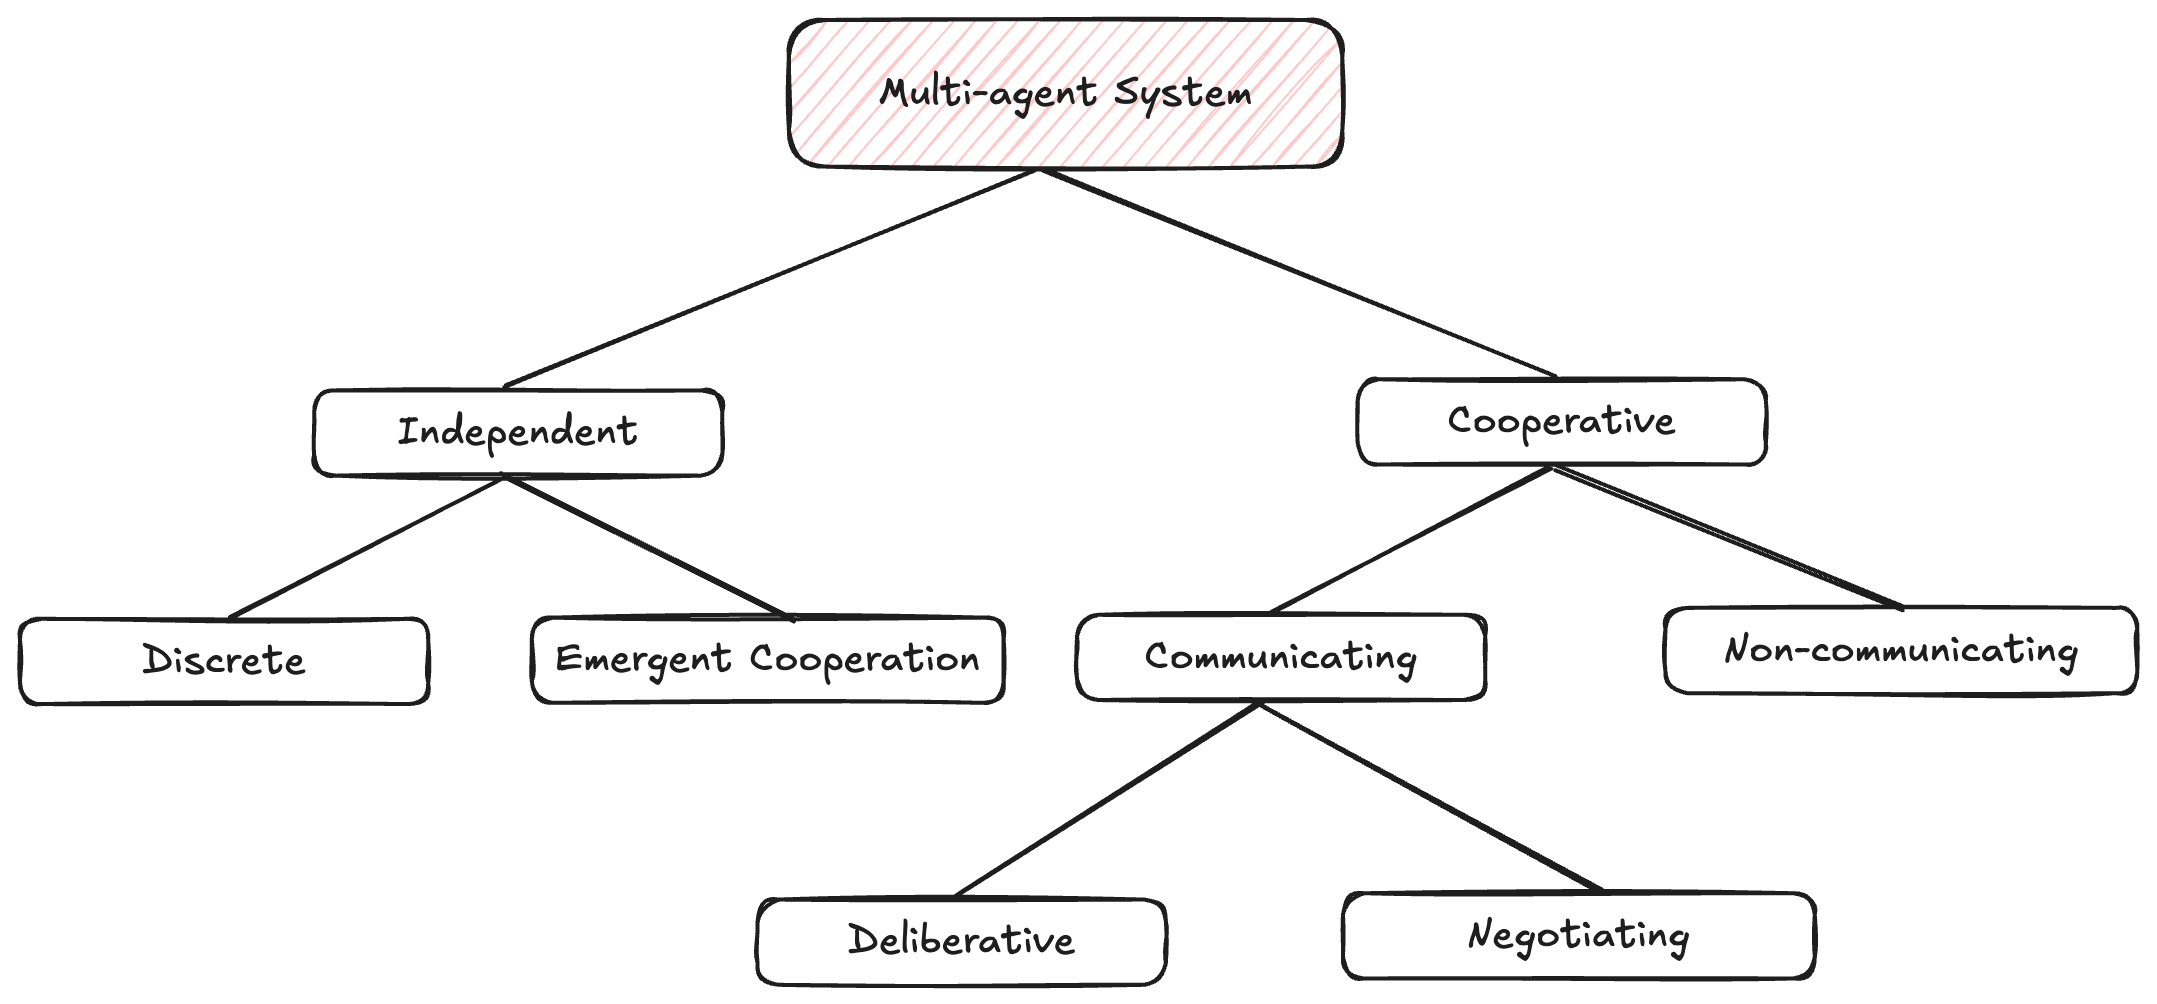
\includegraphics[width=1\linewidth]{img/mas-characteristics.png}
    \caption{\centering\textit{Đặc trưng hệ thống đa tác nhân}}
    \label{fig:mas-characteristics}
\end{figure}

\paragraph{Các kiến trúc phổ biến của hệ thống đa tác nhân}

Cách tổ chức và phối hợp giữa các tác nhân trong một hệ thống MAS được gọi là kiến trúc hệ thống. Kiến trúc quyết định cách các tác nhân giao tiếp, ra quyết định và phối hợp để đạt mục tiêu. Dưới đây là một số kiến trúc phổ biến thường được sử dụng:

\begin{itemize}[topsep=0pt, itemsep=2pt, leftmargin=40pt]
    \item \textbf{Kiến trúc tập trung (Centralized)}: Trong kiến trúc tập trung, một tác nhân trung tâm (central coordinator) quản lý toàn bộ hệ thống và điều phối các tác nhân khác. Cách tiếp cận này đơn giản, dễ kiểm soát nhưng thiếu khả năng chịu lỗi và hạn chế mở rộng khi số lượng tác nhân tăng.
    \item \textbf{Kiến trúc phân tán (Decentralized)}: Ở kiến trúc phân tán, không có tác nhân trung tâm. Các tác nhân phối hợp với nhau theo cơ chế đồng thuận hoặc đàm phán, tự tổ chức để hoàn thành công việc. Đây là kiến trúc phù hợp cho các môi trường phức tạp, nơi tính tự trị và khả năng mở rộng là quan trọng.
    \item \textbf{Mô hình client–server và peer–to–peer}: MAS có thể tổ chức theo mô hình client–server, nơi các tác nhân đóng vai trò rõ ràng là máy khách hoặc máy chủ, hoặc theo mô hình peer–to–peer, nơi các tác nhân ngang hàng, không có phân cấp. Mô hình peer–to–peer giúp hệ thống linh hoạt và dễ mở rộng hơn.
\end{itemize}

\begin{figure}[H]
    \centering
    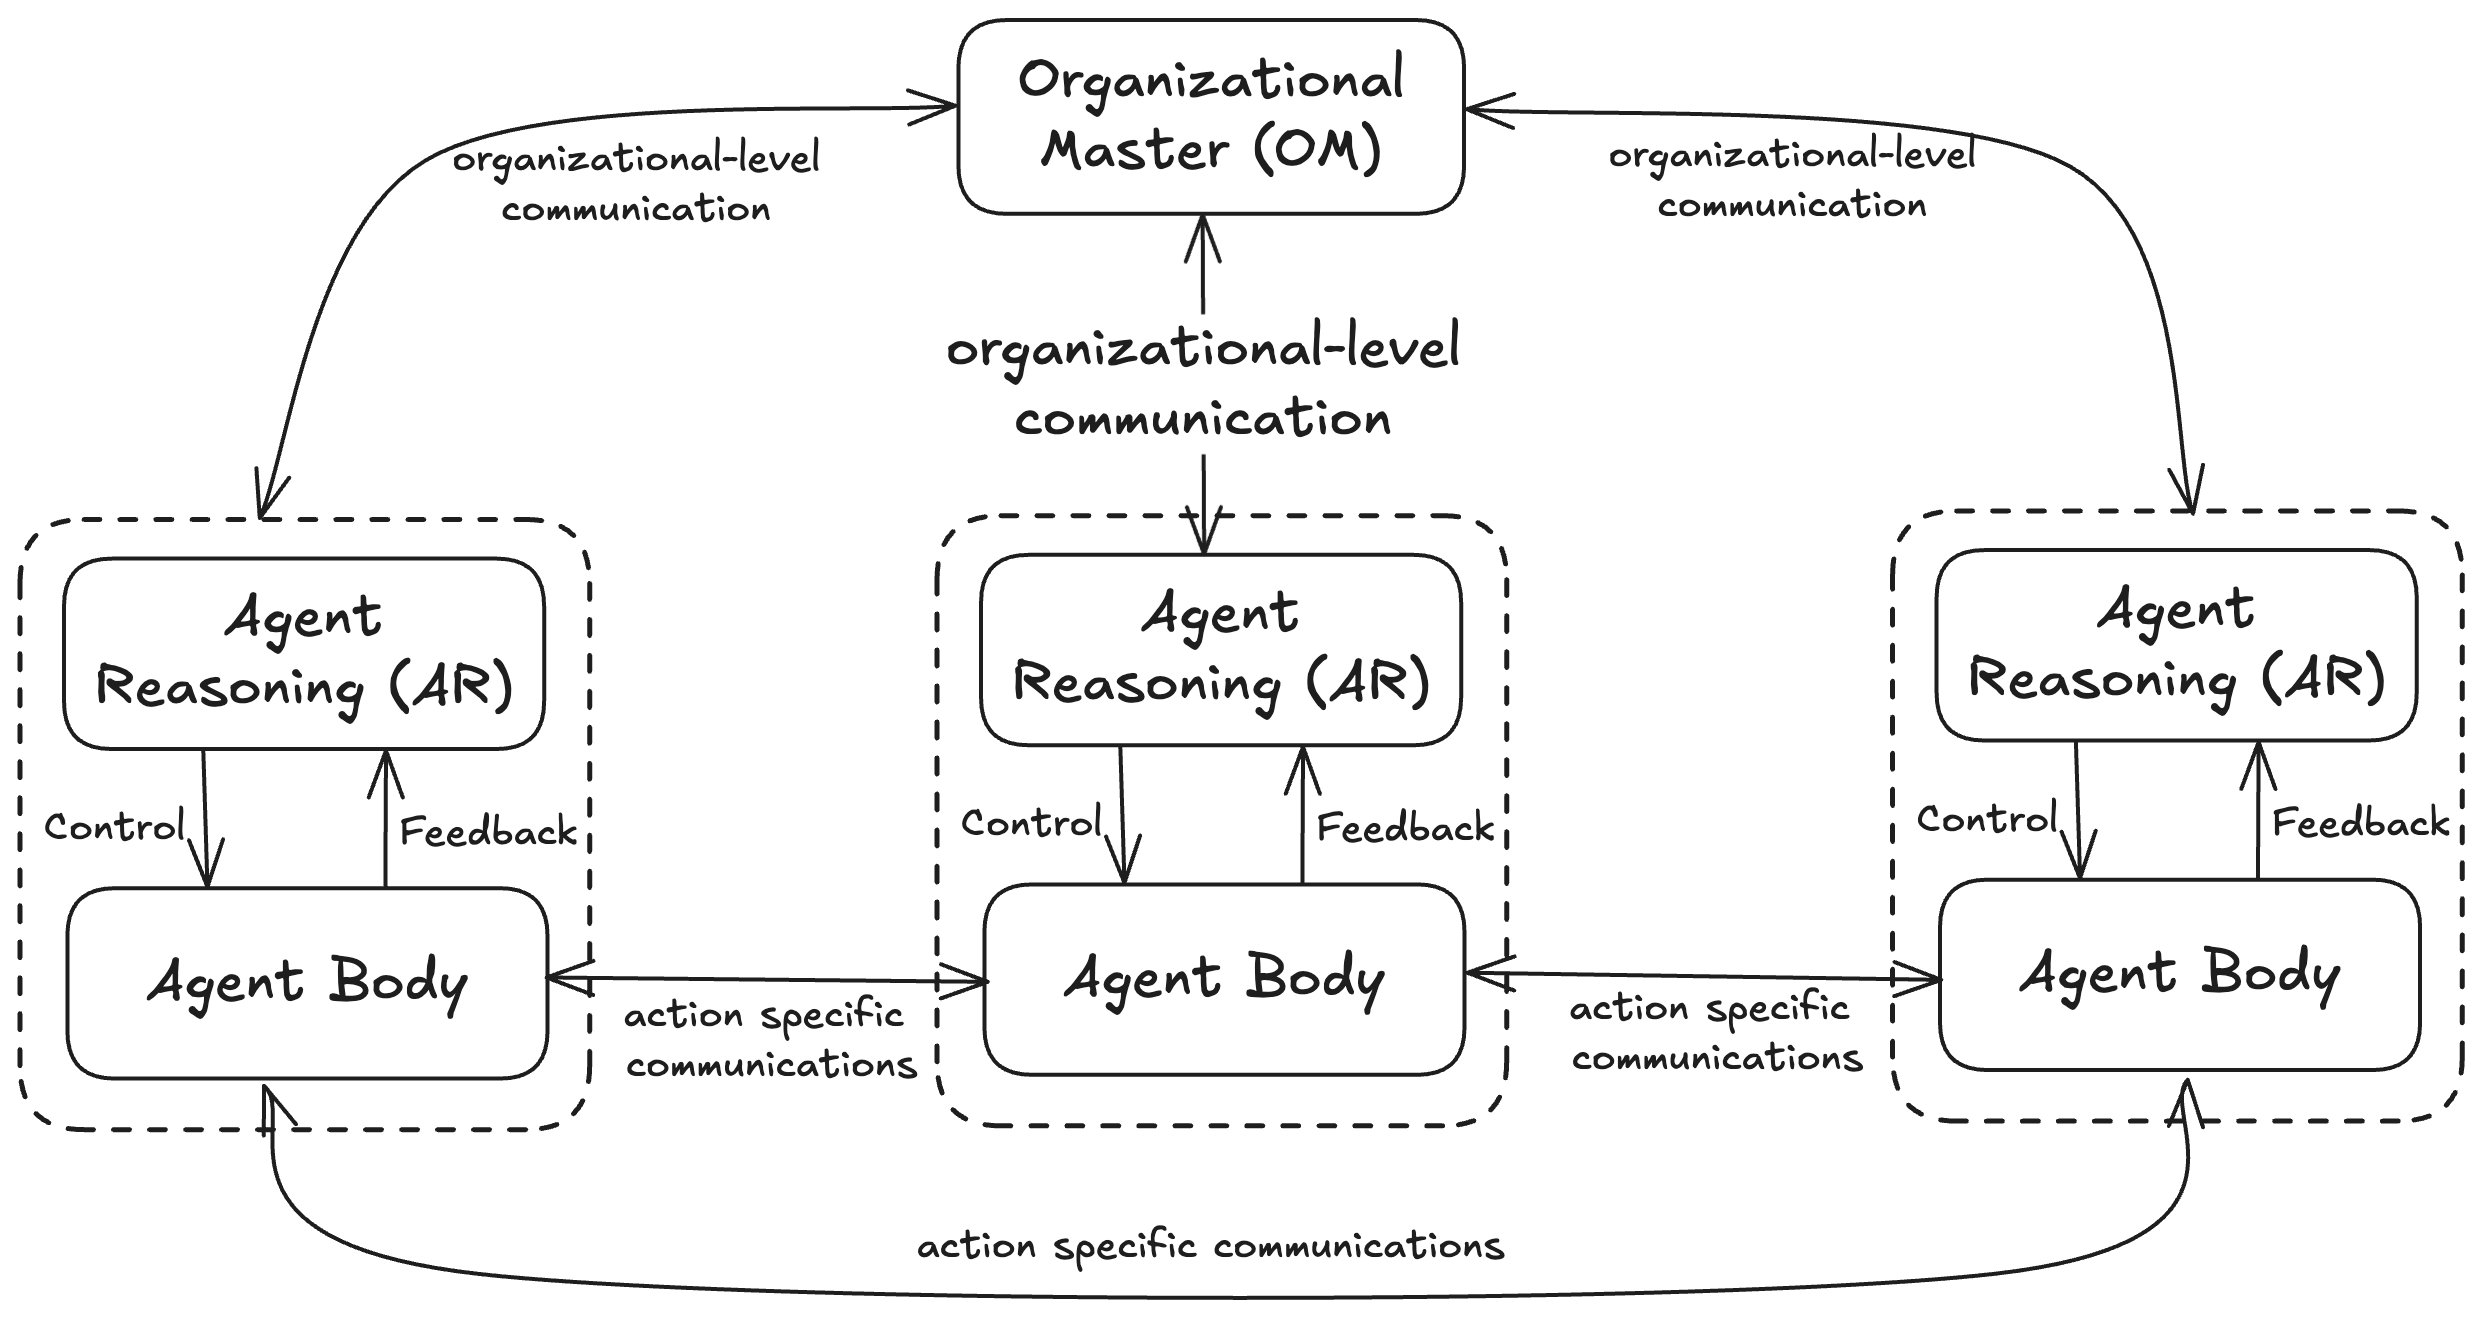
\includegraphics[width=1\linewidth]{img/centralized-mas.png}
    \caption{\centering\textit{Kiến trúc tập trung của hệ thống đa tác nhân}}
    \label{fig:centralized-mas}
\end{figure}

Ngoài các mô hình trên, một số kiến trúc tham khảo cụ thể đã được nghiên cứu và áp dụng, chẳng hạn:

\begin{itemize}[topsep=0pt, itemsep=2pt, leftmargin=40pt]
    \item \textbf{Contract Net Protocol}: các tác nhân đấu thầu và phân chia nhiệm vụ theo hợp đồng.
    \item \textbf{Blackboard Architecture}: các tác nhân đóng góp thông tin vào một bảng chung và truy xuất thông tin từ đó để phối hợp.
    \item \textbf{Holonic MAS}: tổ chức theo dạng "tập thể - cá thể", trong đó mỗi tác nhân vừa là thành phần của tập thể vừa tự chủ.
\end{itemize}

Mỗi kiến trúc có ưu điểm và hạn chế riêng, và việc lựa chọn phụ thuộc vào yêu cầu cụ thể của bài toán, như mức độ phối hợp, độ tin cậy, khả năng mở rộng hay tính động của môi trường.

\subsubsection{Sự can thiệp của con người (Human Intervention)}

Mặc dù các hệ thống đa tác nhân và tác nhân AI có khả năng tự động hóa và ra quyết định độc lập, sự can thiệp của con người vẫn đóng vai trò quan trọng để đảm bảo hệ thống hoạt động hiệu quả, đáng tin cậy và phù hợp với mục tiêu chiến lược của tổ chức. Các hệ thống AI không thể tránh khỏi những hạn chế về dữ liệu, kiến thức chuyên môn hay các yếu tố đạo đức – xã hội, trong khi con người có thể cung cấp phản hồi, điều chỉnh và giám sát dựa trên kinh nghiệm và bối cảnh thực tế.

\begin{figure}[H]
    \centering
    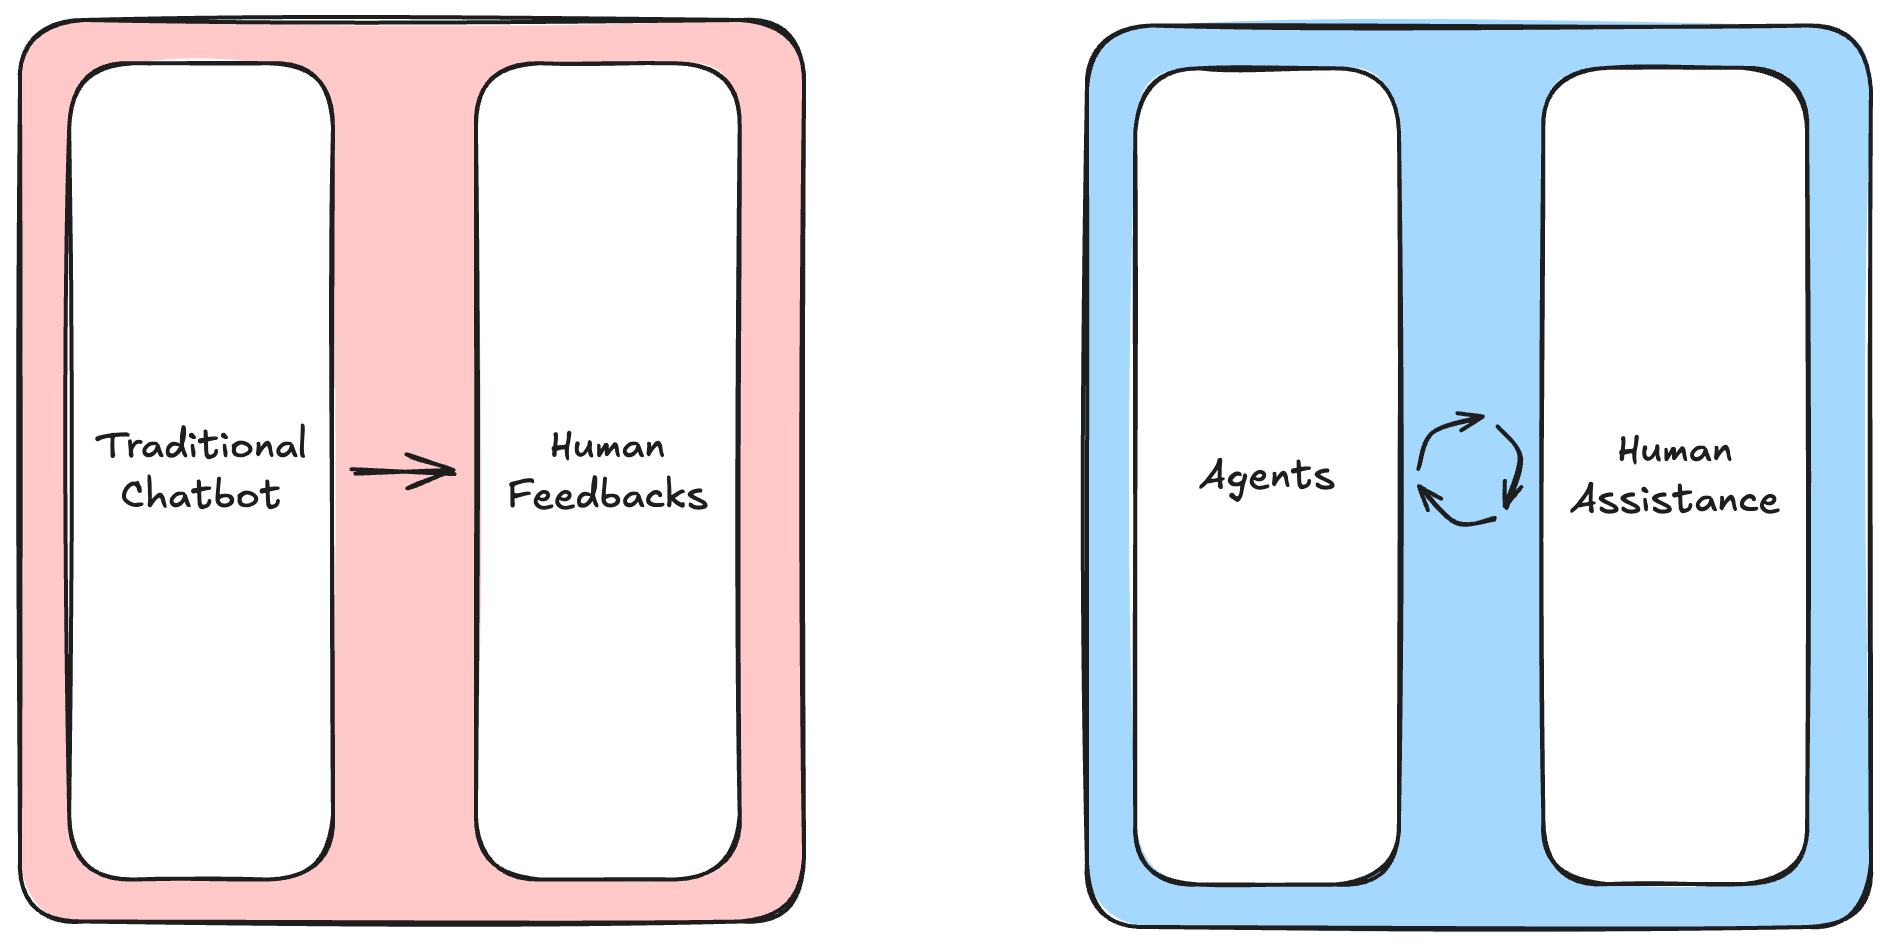
\includegraphics[width=1\linewidth]{img/human-intervention.png}
    \caption{\textit{Sự can thiệp của con người trong tác nhân}}
    \label{fig:human-intervention}
\end{figure}

Trong lĩnh vực quản lý nhân sự, sự kết hợp giữa tự động hóa và can thiệp của con người càng trở nên cần thiết. Các tác nhân AI có thể tự động hóa quy trình thu thập dữ liệu, phân tích và đưa ra gợi ý, nhưng quyết định cuối cùng về tuyển dụng, đánh giá hay đề bạt thường cần đến đánh giá chủ quan, linh hoạt của con người. Hai cơ chế phổ biến để hiện thực hóa sự can thiệp này là \textbf{phản hồi của con người (human feedback)} và \textbf{con người trong vòng lặp (human-in-the-loop)}, giúp hệ thống vừa duy trì tính tự động, vừa đảm bảo chất lượng và tính đúng đắn.

\paragraph{Phản hồi của con người}

Phản hồi của con người (human feedback) là cơ chế cho phép người dùng hoặc chuyên gia góp ý, chỉnh sửa hoặc đánh giá kết quả do hệ thống đưa ra, nhằm cải thiện chất lượng và độ chính xác của tác nhân. Trong các hệ thống MAS áp dụng cho quản lý nhân sự, phản hồi có thể xuất hiện dưới dạng người quản lý đánh giá đề xuất tuyển dụng, chỉnh sửa lịch phỏng vấn hoặc phản biện các đánh giá hiệu suất do hệ thống gợi ý. Tuy nhiên, vì quá trình này thường diễn ra sau khi hệ thống đã hoàn tất một chu trình, nên tính chủ động và mức độ tương tác của con người còn hạn chế so với cách tiếp cận “con người trong vòng lặp”.

\paragraph{Con người trong vòng lặp}

Con người trong vòng lặp (Human-in-the-Loop – HITL) là một cơ chế tương tác chặt chẽ hơn, trong đó con người tham gia trực tiếp vào quá trình ra quyết định của hệ thống trong thời gian thực hoặc theo từng bước quan trọng. Khác với phản hồi thụ động sau khi hệ thống đã hoàn tất, HITL cho phép con người giám sát, can thiệp, và điều chỉnh các tác nhân ngay trong lúc hệ thống đang vận hành. Trong các hệ thống MAS cho quản lý nhân sự, HITL giúp đảm bảo rằng những quyết định nhạy cảm như lựa chọn ứng viên, phân bổ nguồn lực hay đề xuất đào tạo vẫn duy trì yếu tố nhân văn, đồng thời giảm thiểu sai sót hoặc thiên lệch của tác nhân. Cơ chế này đặc biệt phù hợp trong các môi trường phức tạp và nhiều rủi ro, nơi tính tự động cần được cân bằng với khả năng phán đoán và kinh nghiệm của con người.

\begin{figure}[H]
    \centering
    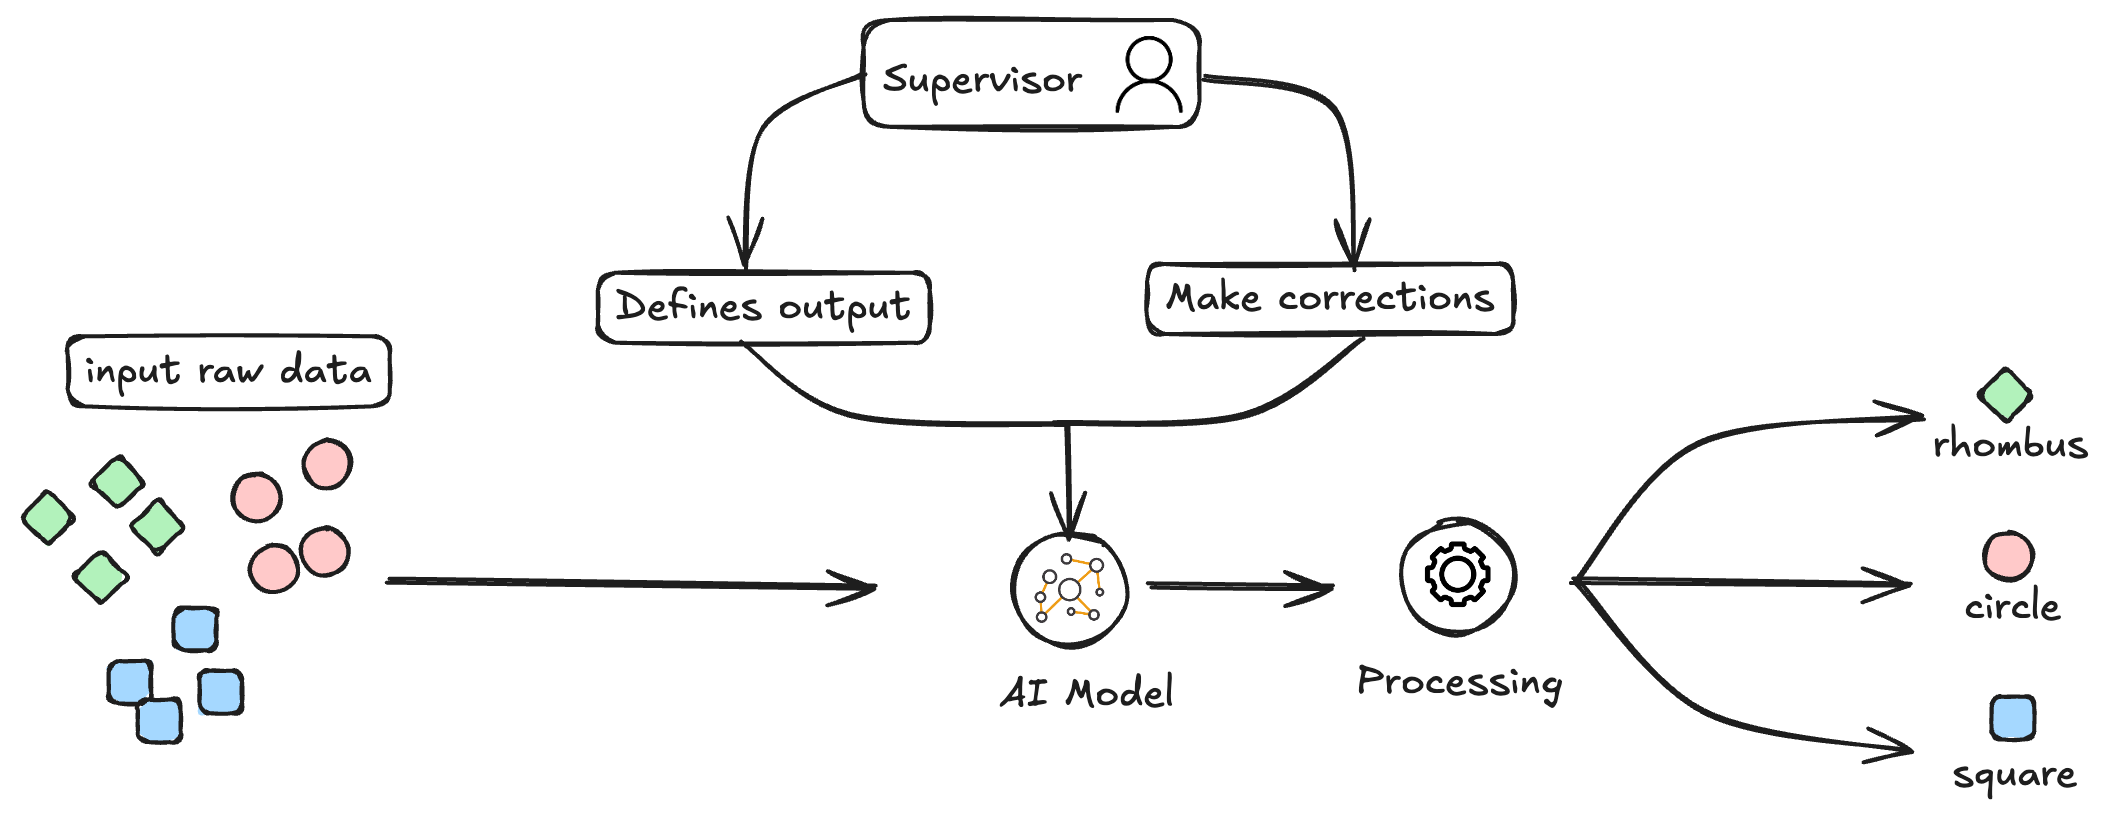
\includegraphics[width=1\linewidth]{img/hitl.png}
    \caption{\centering\textit{Ví dụ HITL trong huấn luyện mô hình AI để phân loại đối tượng}}
    \label{fig:hitl}
\end{figure}

\subsection{Quản trị nhân lực}

Quản trị Nguồn nhân lực (HRM) đã phát triển từ một chức năng hành chính thành một đối tác kinh doanh chiến lược, trong đó Thu hút nhân tài (Talent Acquisition – TA) đóng vai trò then chốt. Thay vì chỉ tuyển dụng để lấp đầy vị trí trống, TA tập trung vào các hoạt động dài hạn như xây dựng thương hiệu nhà tuyển dụng và phát triển các kênh ứng viên tiềm năng để đảm bảo lợi thế cạnh tranh. Tuy nhiên, các đội ngũ TA ngày nay phải đối mặt với nhiều thách thức như thiếu hụt nhân tài, không tương thích về kỹ năng và quy trình tuyển dụng kém hiệu quả, với thời gian tuyển dụng trung bình kéo dài tới 43 ngày trong khi các ứng viên hàng đầu thường được tuyển dụng chỉ trong 10 ngày.

\subsubsection{Hệ thống ATS truyền thống và những hạn chế}
Hệ thống \textit{Applicant Tracking System} (ATS) đã trở thành tiêu chuẩn trong quy trình tuyển dụng hiện đại, hỗ trợ doanh nghiệp tự động hoá khâu thu thập, lưu trữ và tìm kiếm hồ sơ ứng viên. Nhờ cơ chế lọc dựa trên từ khóa, ATS có thể giảm khối lượng công việc thủ công cho chuyên viên nhân sự và đẩy nhanh quá trình sàng lọc sơ bộ.

Tuy nhiên, các ATS truyền thống bộc lộ nhiều hạn chế: 
\begin{enumerate}[topsep=0pt, itemsep=2pt, leftmargin=40pt, label=\arabic*.]
    \item Phụ thuộc nặng vào đối sánh từ khoá khiến hồ sơ chứa thuật ngữ bất quy tắc hoặc mô tả kỹ năng sắc thái dễ bị loại bỏ, làm gia tăng \textit{False Negative}.
    \item Thuật toán xếp hạng thường không xét đến mức độ phù hợp ngữ cảnh, dẫn tới thiên lệch đối với mẫu CV “chuẩn” và tái tạo định kiến tuyển dụng.
    \item Khả năng “học” gần như bằng không, nên hệ thống khó thích nghi với yêu cầu năng lực mới hoặc phản hồi từ chuyên viên.
\end{enumerate}

Hệ quả là doanh nghiệp bỏ lỡ nhân tài tiềm ẩn, trong khi chuyên viên vẫn phải can thiệp sâu ở các bước sau. Những thách thức này sẽ được phân tích chi tiết hơn trong Chương 3 nhằm làm rõ động lực xây dựng một kiến trúc tuyển dụng thông minh dựa trên LLM và hệ đa tác nhân.

\subsubsection{Vai trò của Thu hút nhân tài (Talent Acquisition)}
Khác với khái niệm tuyển dụng thuần tuý, Thu hút nhân tài (Talent Acquisition – TA) là một chức năng mang tính chiến lược, bao hàm toàn bộ vòng đời của nhân tài từ giai đoạn nhận diện, tương tác, đánh giá cho tới phát triển. Mục tiêu cốt lõi của TA không chỉ là lấp đầy vị trí trống nhanh nhất mà còn đảm bảo doanh nghiệp luôn duy trì một “pipeline” ứng viên chất lượng cao, phù hợp với tầm nhìn dài hạn cũng như năng lực cạnh tranh cốt lõi.

Tầm quan trọng của TA thể hiện ở ba khía cạnh chủ đạo. Thứ nhất, TA gắn liền với xây dựng thương hiệu nhà tuyển dụng, giúp gia tăng khả năng thu hút ứng viên thụ động – nhóm chiếm tới 70\% lực lượng lao động toàn cầu. Thứ hai, TA giảm thiểu rủi ro thiếu hụt kỹ năng trong tương lai bằng cách liên tục lập bản đồ thị trường nhân sự và chủ động tương tác với các nhóm nhân tài trọng yếu. Cuối cùng, TA cung cấp nguồn dữ liệu phong phú (ứng viên, thị trường, hiệu suất kênh) giúp HRM ra quyết định dựa trên dữ liệu, qua đó rút ngắn \textit{time-to-hire}, nâng cao \textit{quality-of-hire} và tối ưu chi phí. Vì vậy, các giải pháp công nghệ hướng tới tự động hoá sàng lọc và khai thác dữ liệu – như hệ thống đa tác nhân dựa trên LLM mà luận văn đề xuất – cần đặt TA làm trọng tâm thiết kế.

\subsubsection{Khung lý thuyết cho việc đánh giá}
Để đánh giá hiệu quả của hệ thống, luận văn sử dụng các chỉ số tiêu chuẩn từ lý thuyết phân loại và truy xuất thông tin, phản ánh các mục tiêu kép là giảm thất thoát nhân tài và giảm tải công việc cho chuyên viên.

\paragraph{Đo lường khả năng Thu hồi Nhân tài}

Nhiệm vụ sàng lọc về cơ bản là một bài toán phân loại nhị phân, do đó có thể được đánh giá bằng các chỉ số \textbf{Độ chính xác (Precision)} và \textbf{Độ thu hồi (Recall)}. Trong bối cảnh tuyển dụng, việc bỏ lỡ một ứng viên giỏi (một Âm tính giả – False Negative) có chi phí cơ hội rất cao. Do đó, \textbf{Recall}, tức tỷ lệ các ứng viên thực sự đủ điều kiện mà hệ thống tìm thấy, là chỉ số quan trọng nhất. \textbf{Tỷ lệ Loại sai (False Rejection Rate – FRR)}, tức tỷ lệ ứng viên đủ điều kiện bị hệ thống loại bỏ sai, có mối quan hệ nghịch đảo trực tiếp với Recall. Do đó, mục tiêu tối đa hóa Recall tương đương về mặt toán học với việc tối thiểu hóa FRR.
\begin{align*}
\text{Recall} &=\frac{\text{TP}}{\text{TP} + \text{FN}} \\
\text{Precision}&= \frac{\text{TP}}{\text{TP} + \text{FP}} \\
\text{FRR} &=\frac{\text{FN}}{\text{TP} + \text{FN}} = 1 - \text{Recall}
\end{align*}

\paragraph{Định lượng Nỗ lực của Chuyên viên}
Để đo lường mức độ giảm tải công việc, luận văn đề xuất \textbf{Chỉ số Giảm tải Đánh giá (Reviewer Load Reduction – RLR)}, lấy cảm hứng từ khái niệm "công việc được tiết kiệm" trong các nghiên cứu y khoa. Chỉ số này định lượng phần trăm công việc sàng lọc thủ công mà hệ thống đã loại bỏ cho chuyên viên. Một hệ thống thành công phải đạt được Recall cao trong khi vẫn giữ cho RLR ở mức cao, nghĩa là tìm thấy hầu hết các ứng viên giỏi trong khi chỉ yêu cầu chuyên viên xem xét một phần nhỏ trong tổng số hồ sơ.
\begin{align*}
\text{RLR} = 1-\frac{\text{Số lượng hồ sơ ứng viên cần xem xét}}{\text{Tổng hồ sơ ứng tuyển}}
\end{align*}

\subsection{Các chỉ số thống kê}
\subsubsection{Giá trị p (p-value)}
Giá trị $p$ là một chỉ số trong kiểm định giả thuyết thống kê, dùng để xác định ý nghĩa của kết quả quan sát được. Nó biểu thị xác suất thu được một kết quả ít nhất là cực đoan như kết quả thực tế, với giả định rằng giả thuyết không ($H_0$) là đúng. Trong bối cảnh của luận văn này, giả thuyết không cho rằng không có sự khác biệt thực sự về Tỷ lệ Loại nhầm (FRR) giữa hệ thống mới và hệ thống truyền thống. Một giá trị $p$ nhỏ (thường là $p<0.05$) cho phép bác bỏ giả thuyết không, cung cấp bằng chứng thống kê rằng sự cải thiện quan sát được (ví dụ: FRR giảm) không phải do ngẫu nhiên mà là một hiệu ứng thực sự của hệ thống.

\subsubsection{Kích thước hiệu ứng (Cohen's h)}
Trong khi giá trị $p$ cho biết liệu sự khác biệt có ý nghĩa thống kê hay không, nó không cho biết mức độ lớn của sự khác biệt đó. Kích thước hiệu ứng Cohen's $h$ được sử dụng để định lượng sự khác biệt giữa hai tỷ lệ độc lập (ví dụ: so sánh FRR của hai hệ thống). Chỉ số này giúp xác định ý nghĩa thực tiễn của kết quả. Công thức tính Cohen's $h$ là:
\begin{gather*}
h = 2(\arcsin\sqrt{P_1} -\arcsin\sqrt{P_2})
\end{gather*}

trong đó $P_1$ và $P_2$ là hai tỷ lệ được so sánh. Theo quy ước, giá trị h được diễn giải như sau: $h=0.2$ (hiệu ứng nhỏ), $h=0.5$ (hiệu ứng trung bình), và $h=0.8$ (hiệu ứng lớn).

\subsubsection{Hệ số Cohen's Kappa}
Hệ số Cohen's Kappa ($\kappa$) là một thước đo thống kê về mức độ đồng thuận giữa hai người đánh giá (inter-rater reliability) đối với các mục phân loại, trong khi hiệu chỉnh cho sự đồng thuận có thể xảy ra do ngẫu nhiên. Trong nghiên cứu này, Kappa có thể được dùng để đo lường mức độ nhất quán giữa các quyết định của hệ thống và các nhãn "sự thật nền" (ground-truth) được gán bởi chuyên gia nhân sự. Một giá trị $\kappa$ cao cho thấy hệ thống không chỉ đưa ra quyết định chính xác mà còn có mức độ tin cậy và nhất quán cao, tương tự như một chuyên gia con người. Công thức được định nghĩa là:

\begin{gather*}
\kappa = \frac{p_o-p_e}{1-p_e}
\end{gather*}
trong đó $p_o$ là tỷ lệ đồng thuận quan sát được và $p_e$ là xác suất đồng thuận do ngẫu nhiên. Giá trị Kappa gần 1 cho thấy sự đồng thuận hoàn hảo, trong khi giá trị gần 0 cho thấy sự đồng thuận không tốt hơn so với ngẫu nhiên.

\subsection{Tổng kết chương}
Chương này đã thiết lập một nền tảng lý thuyết và công nghệ toàn diện. Phần đầu tiên đã giới thiệu các công nghệ nền tảng, bao gồm LLM, Tác nhân AI, kiến trúc Hệ Đa tác nhân và sự can thiệp của con người trong hệ thống tác nhân. Những khái niệm này cung cấp bộ công cụ kỹ thuật để xây dựng một giải pháp thông minh và tự chủ.

Phần tiếp theo mô tả sự chuyển đổi của HRM từ chức năng hành chính sang vai trò đối tác chiến lược, xác định Thu hút nhân tài (TA) là trung tâm; tiếp đó phân tích các hạn chế cố hữu của hệ thống Applicant Tracking System (ATS) truyền thống—phụ thuộc đối sánh từ khóa, thiếu khả năng học hỏi và tiềm ẩn thiên lệch—từ đó nhấn mạnh nhu cầu về một giải pháp tiên tiến hơn. Chương nêu bật tầm quan trọng của TA trong xây dựng thương hiệu tuyển dụng, phòng ngừa thiếu hụt kỹ năng và cung cấp dữ liệu ra quyết định. Cuối cùng, một khung đánh giá chặt chẽ dùng hai chỉ số FRR và RLR được thiết lập nhằm đo lường đồng thời khả năng thu hồi nhân tài và mức độ giảm tải cho chuyên viên, tạo nền tảng lý thuyết vững chắc dẫn hướng thiết kế–kiểm nghiệm hệ thống ở các chương tiếp theo.

\newpage

\titleformat{\section}{\fontsize{28pt}{8pt}\bfseries}{}{0pt}{%
    {\fontsize{20pt}{0pt}\selectfont Chương \thesection}\\[16pt]%
    {}%
}
\tocless\section{Phương pháp nghiên cứu}
\addcontentsline{toc}{section}{\numberline{}CHƯƠNG 3: PHƯƠNG PHÁP NGHIÊN CỨU}
\setcounter{section}{3}

Chương này trình bày phương pháp nghiên cứu nhằm phát triển và đánh giá Hệ thống Đa Tác Nhân (Multi-Agent System – MAS) sử dụng trí tuệ nhân tạo cho mục tiêu tự động hoá quy trình thu hút nhân tài (Talent Acquisition). Phương pháp luận được xây dựng theo hướng tiếp cận hỗn hợp (mixed-methods), kết hợp:
\begin{enumerate}[topsep=0pt, itemsep=2pt, leftmargin=40pt, label=\arabic*.]
    \item Tổng quan tài liệu có hệ thống.
    \item Phân tích so sánh các hệ thống hiện hành.
    \item Xác định bộ chỉ số định lượng.
    \item Nghiên cứu thiết kế dành cho giải pháp đa tác nhân đề xuất.
\end{enumerate}

Mục tiêu nghiên cứu là khắc phục tỉ lệ loại nhầm ứng viên đủ điều kiện (false rejection rate) ở mức 12–35\% của các Hệ thống Theo dõi Ứng viên (Applicant Tracking Systems – ATS) hiện nay, thông qua kiến trúc đa tác tử có con người tham gia trong vòng lặp (human-in-the-loop – HITL).

\vspace{14pt}
\setcounter{subsection}{0}
\setcounter{table}{0}
\setcounter{figure}{0}
\subsection{Phân tích căn nguyên thất bại của hệ thống ATS}
Các hệ thống ATS hiện đang xử lý trên 75\% tổng số hồ sơ xin việc tại các doanh nghiệp lớn. Tuy nhiên, một thực trạng đáng báo động là có từ 12\% đến 35\% ứng viên đủ tiêu chuẩn không bao giờ tiếp cận được nhà tuyển dụng do bị hệ thống loại nhầm. Tỷ lệ sai sót nghiêm trọng này (FRR) không phải là lỗi cấu hình đơn lẻ mà là một yếu điểm mang tính hệ thống, cố hữu trong kiến trúc của hầu hết các nền tảng ATS hiện nay.

Tiểu mục này sẽ chứng minh bản chất hệ thống của vấn đề thông qua việc phân tích và so sánh hai nền tảng ATS phổ biến, chỉ ra ba khiếm khuyết thiết kế cốt lõi. Từ đó, tác động và thiệt hại kinh tế của tỷ lệ loại nhầm này sẽ được lượng hóa, ước tính thiệt hại có thể lên đến từ $750\,000$ đến $3.45$ triệu USD cho mỗi 100 vị trí được tuyển dụng hàng năm.

\subsubsection{Nguyên lý hoạt động và hạn chế của các hệ thống ATS hiện hành}
Để lý giải nguyên nhân các hệ thống ATS hiện hành thường xuyên loại bỏ ứng viên đủ điều kiện, mục này tập trung phân tích logic vận hành và chỉ ra các giai đoạn cốt lõi nơi sai sót xảy ra một cách có hệ thống. Phương pháp tiếp cận bao gồm việc nghiên cứu hai nền tảng tiêu biểu, so sánh cơ chế sàng lọc và phân rã quy trình tổng quát để làm rõ nguồn gốc của tỉ lệ FRR cao đã được ghi nhận.

\paragraph{Cơ sở lựa chọn và phân tích so sánh}
Nghiên cứu lựa chọn hai hệ thống ATS tiêu biểu là \textbf{Taleo (1999)} và \textbf{Lever (2012)}. Dù thuộc hai thế hệ công nghệ khác nhau, cả hai nền tảng này đều đại diện cho phần lớn thị trường và cùng chia sẻ một logic sàng lọc nền tảng: \textbf{đối sánh từ khóa chính xác (exact keyword matching)}. Sự tương đồng về kiến trúc lõi này cho phép khẳng định rằng các sai sót trong việc sàng lọc ứng viên bắt nguồn từ những hạn chế trong thiết kế chung của hệ thống, chứ không đơn thuần là lỗi cấu hình hay giao diện riêng lẻ.

\paragraph{Phân tích so sánh hai nền tảng ATS điển hình}
\begin{longtable}{|
  % Table columns define
  >{\raggedright\arraybackslash}p{0.18\textwidth}|
  >{\raggedright\arraybackslash}p{0.29\textwidth}|
  >{\raggedright\arraybackslash}p{0.2\textwidth}|
  >{\raggedright\arraybackslash}p{0.23\textwidth}|}
  % Table columns define end here.
  \hline
  % Table header start from here, should modify if needed
  \textbf{Nền tảng} & 
  \textbf{Cơ chế sàng lọc cốt lõi} & 
  \textbf{Tỷ lệ loại nhầm (FRR) đo được} & 
  \textbf{Ví dụ ứng viên bị loại} \\
  \hline
  % Table header end here.
  \endfirsthead

  % No header on continuation pages
  \endhead

  \hline
  \endfoot

  \hline
  \caption{\textit{So sánh hai nền tảng ATS}} \\
  \endlastfoot

  Taleo / Oracle & 
  Lọc từ khóa Boolean, đối sánh chính xác tuyệt đối (1999) & 
  40–60\% & 
  Ứng viên ghi “PL/SQL” bị loại cho vị trí yêu cầu “SQL” \\
  \hline

  Lever & 
  Luật từ khóa do nhà tuyển dụng định nghĩa, giao diện hiện đại (2012) & 
  ≈ 45\% (với hồ sơ phi truyền thống) & 
  Kinh nghiệm làm việc “overseas” (nước ngoài) bị đánh dấu không liên quan cho vị trí yêu cầu khu vực “EMEA” \\
  \hline
  
\end{longtable}

\hyperref[tab:ats-comparison]{\color{blue}{Bảng 3.1}} tổng hợp các đặc tính kiến trúc và những kiểu thất bại đã được ghi nhận của hai hệ thống. Dữ liệu cho thấy, dù có khoảng cách 13 năm về công nghệ, cả hai nền tảng đều bộc lộ "điểm mù" cố hữu về từ đồng nghĩa và ngữ cảnh. Điều này củng cố cho kết luận rằng tỷ lệ loại nhầm từ 12-35\% được công bố bởi các nghiên cứu trước đây là một hạn chế mang tính kiến trúc, chứ không phải một sai sót cá biệt.

\paragraph{Phân rã quy trình và các điểm gây thất thoát nhân tài}
Hạn chế về kiến trúc của ATS trở nên rõ ràng hơn khi phân rã một quy trình tuyển dụng điển hình thành các giai đoạn tuần tự. \hyperref[fig:ats-diagram]{\color{blue}{Hình 3.1}} mô hình hóa một "phễu" tuyển dụng của doanh nghiệp Fortune 500, nơi một vị trí thu hút trung bình 250 hồ sơ và chỉ có một phần rất nhỏ đến được tay nhà tuyển dụng. Quy trình này bộc lộ ba giai đoạn chính gây ra sự loại bỏ có hệ thống, tương ứng với ba loại lỗi đo lường được ($E_1$, $E_2$, $E_3$ và $E_4$).

\begin{figure}[H]
    \centering
    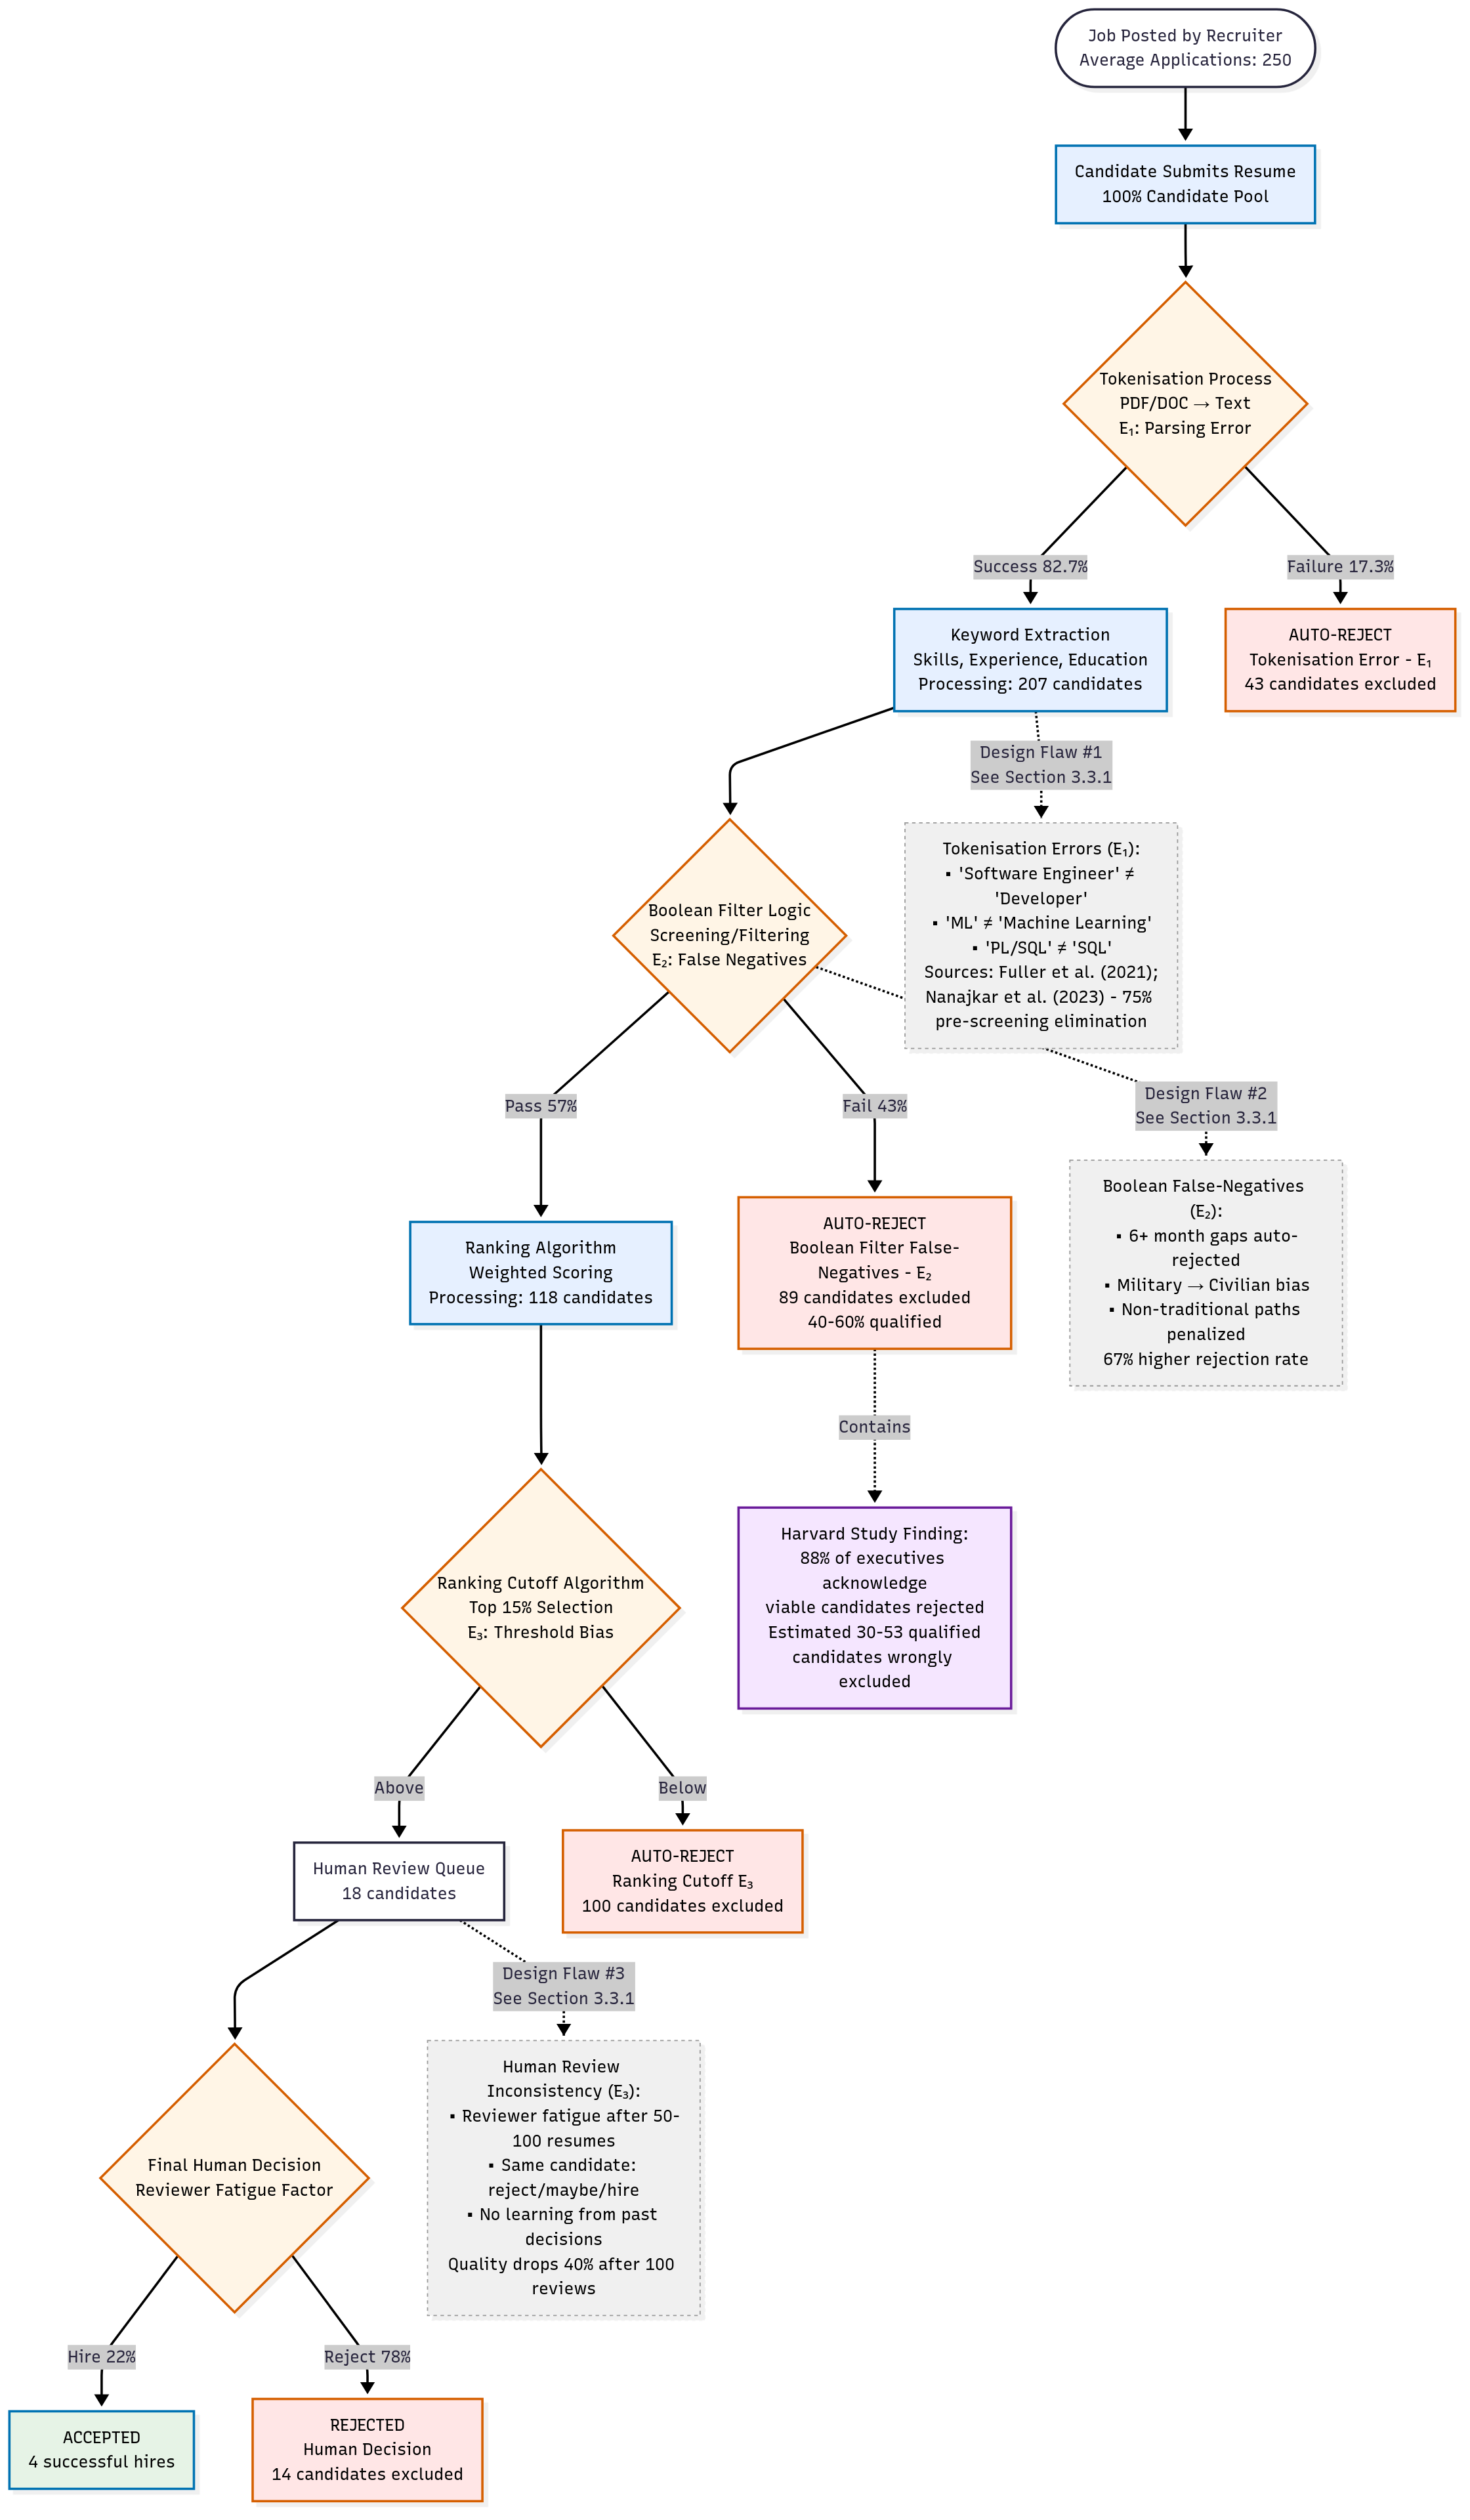
\includegraphics[width=0.8\linewidth]{img/ats-diagram.png}
    \caption{\textit{Cơ chế loại bỏ có hệ thống trong quy trình tự động sàng lọc ứng viên}}
    \label{fig:ats-diagram}
\end{figure}

\begin{enumerate}[topsep=0pt, itemsep=2pt, leftmargin=40pt, label=$E_{\arabic*}$.]
    \item \textbf{Phân tích cú pháp tài liệu – Token hóa}: Ngay từ bước đầu tiên, khoảng 17\% hồ sơ (43 trên 250) bị loại bỏ hoàn toàn do các lỗi kỹ thuật. Nguyên nhân là hệ thống không thể phân tích (parse) các tệp có định dạng không chuẩn như PDF phức tạp hoặc ảnh được quét. Việc loại bỏ này dựa trên định dạng tệp thay vì năng lực ứng viên, tạo ra lớp thất thoát nhân tài đầu tiên một cách vô lý.
    \item \textbf{Lọc từ khóa Boolean}: Trong số các hồ sơ được phân tích thành công, có thêm 43\% (khoảng 89 hồ sơ) bị loại vì các từ khóa trong CV không khớp chính xác với bộ lọc của nhà tuyển dụng. Các phân tích chuyên sâu chỉ ra rằng 40-60\% trong số này thực chất là ứng viên đủ tiêu chuẩn. Đây chính là nguồn gây ra tỷ lệ loại nhầm lớn nhất, bắt nguồn từ việc hệ thống không hiểu được các thuật ngữ tương đương về mặt ngữ nghĩa (ví dụ: "ML" và "Machine Learning").
    \item \textbf{Xếp hạng theo trọng số \& Thiết lập ngưỡng}: Các hồ sơ còn lại được chấm điểm và xếp hạng, sau đó một ngưỡng cắt cứng (thường là top 15\%) được áp dụng để chọn ra danh sách rút gọn. Điều này dẫn đến việc khoảng 100 ứng viên "cận ngưỡng" bị loại bỏ, dù chênh lệch điểm số có thể không đáng kể (<1\%). Giai đoạn này tiếp tục làm gia tăng sự thất thoát nhân tài một cách máy móc.
    \item \textbf{Nhà tuyển dụng đánh giá}: Cuối cùng, chỉ chưa đến 8\% tổng số hồ sơ ban đầu được chuyển đến cho nhà tuyển dụng xem xét thủ công. Ở giai đoạn này, sự mệt mỏi về nhận thức và các tiêu chí chủ quan tiếp tục làm giảm tính nhất quán, với hệ số đồng thuận giữa những người đánh giá (inter-rater agreement) được ghi nhận ở mức rất thấp ($k\approx 0.31$).
\end{enumerate}
Tóm lại, quy trình sàng lọc tự động của các hệ thống ATS hiện hành chứa đựng những khiếm khuyết mang tính hệ thống ở nhiều giai đoạn, từ phân tích kỹ thuật đến lọc logic và xếp hạng. Trong đó, sự phụ thuộc vào logic từ khóa Boolean ($E_2$) là yếu điểm kiến trúc nổi trội nhất, gây ra phần lớn sự thất thoát các ứng viên tiềm năng. Phân tích này cung cấp một nền tảng thực nghiệm vững chắc để đề xuất một kiến trúc thay thế trong các chương tiếp theo.

\subsubsection{Tác động có hệ thống của Tỷ lệ Loại nhầm: Từ Bằng chứng Thực nghiệm đến Thiệt hại Kinh tế}
Trong khi mục trước đã phân rã cơ chế vận hành dẫn đến thất bại của hệ thống ATS, mục này sẽ đi sâu vào việc lượng hóa quy mô và tác động của những sai sót đó. Bằng cách tổng hợp các bằng chứng thực nghiệm và phân tích chi phí kinh doanh, luận văn sẽ chứng minh rằng tỷ lệ FRR không chỉ là một khiếm khuyết kỹ thuật, mà còn là một gánh nặng chiến lược và kinh tế đáng kể đối với các tổ chức.

\paragraph{Bằng chứng thực nghiệm về quy mô của vấn đề}
Nhiều nghiên cứu liên ngành đã hội tụ tại một kết luận nhất quán: logic sàng lọc dựa trên từ khóa của các hệ thống ATS truyền thống đang tạo ra một tỷ lệ FRR cao và có hệ thống. Nghiên cứu nền tảng "Hidden Workers" của Trường Kinh doanh Harvard, thực hiện trên 2,847 nhà quản lý tuyển dụng, đã chỉ ra rằng 88\% người được hỏi thừa nhận hệ thống ATS của họ "thường xuyên loại bỏ các ứng viên đủ tiêu chuẩn" do các bộ lọc cứng nhắc. Phân tích định lượng trong cùng nghiên cứu này xác định tỷ lệ FRR dao động trong khoảng 12\% đến 35\%, tùy thuộc vào cấu hình hệ thống và mức độ giám sát của con người.

Phát hiện này không phải là một trường hợp cá biệt. Các bằng chứng từ nhiều nguồn uy tín khác đã củng cố và làm rõ thêm các cơ chế gây ra sai sót này:
\begin{longtable}{|
  % Table columns define
  >{\raggedright\arraybackslash}p{0.25\textwidth}|
  >{\raggedright\arraybackslash}p{0.35\textwidth}|
  >{\raggedright\arraybackslash}p{0.35\textwidth}|}
  % Table columns define end here.
  \hline
  % Table header start from here, should modify if needed
  \textbf{Nguồn} &
  \textbf{Phát hiện chính} &
  \textbf{Hàm ý} \\
  \hline
  % Table header end here.
  \endfirsthead

  % No header on continuation pages
  \endhead

  \hline
  \endfoot

  \hline
  \caption{\textit{Bằng chứng hội tụ về các hạn chế của ATS}} \\
  \endlastfoot

  OECD Employment Outlook (2023) &
  $50\%$ doanh nghiệp tự động loại bỏ ứng viên có khoảng trống kinh nghiệm làm việc từ 6 tháng trở lên. &
  Tạo ra thiên kiến có hệ thống đối với những người chuyển đổi sự nghiệp, người tạm nghỉ để chăm sóc gia đình, hoặc sinh viên mới ra trường. \\
  \hline

  ManpowerGroup (2024) &
  $75\%$ nhà tuyển dụng báo cáo gặp khó khăn trong việc tuyển dụng dù thị trường vẫn có nhân tài. &
  Tình trạng "thiếu hụt nhân tài" mang tính nhân tạo — ứng viên tiềm năng vẫn tồn tại nhưng đã bị hệ thống lọc bỏ. \\
  \hline

  LinkedIn Talent Solutions (2023) &
  $54\%$ người dùng hệ thống Taleo (một ATS hàng đầu) đánh giá hệ thống tuyển dụng của họ "kém hiệu quả". &
  Ngay cả người dùng của những hệ thống dẫn đầu thị trường cũng thừa nhận hiệu suất hoạt động thấp. \\
  \hline

  Nghiên cứu Kỹ thuật của IEEE (2023) &
  Thiên kiến giới trong thuật toán tuyển dụng đã loại bỏ một cách có hệ thống các ứng viên nữ đủ tiêu chuẩn. &
  Cung cấp bằng chứng từ góc độ kỹ thuật về sự phân biệt đối xử trong hoạt động tuyển dụng dựa trên thuật toán. \\
  \hline
\end{longtable}

Về mặt kỹ thuật, những sai sót này bắt nguồn từ các cơ chế thiên vị đã được lập trình sẵn. Ví dụ, công cụ tuyển dụng AI của Amazon (hiện đã ngừng sử dụng) đã "học" cách đánh giá tiêu cực các hồ sơ của ứng viên nữ sau khi được huấn luyện trên dữ liệu lịch sử vốn có tỷ lệ nam giới chiếm đa số. Tương tự, các lỗi trong đối sánh từ khóa (keyword matching failures) và phân tích định dạng (format parsing bias) cũng góp phần loại bỏ một cách có hệ thống các ứng viên có kinh nghiệm liên quan nhưng sử dụng thuật ngữ khác hoặc có định dạng hồ sơ phi tiêu chuẩn. Như chuyên gia Jelena Kovačević (IEEE Fellow) giải thích: \textit{"Nếu một tập dữ liệu thiếu tính đa dạng, thuật toán AI được xây dựng dựa trên nó sẽ kế thừa sự thiên vị đó."}

\paragraph{Lượng hóa tác động kinh tế}
Để chuyển đổi tỷ lệ FRR từ 12-35\% thành chi phí kinh doanh cụ thể, ta có thể sử dụng phép so sánh với hiện tượng "chiếc xô bị rò rỉ". Quá trình tuyển dụng giống như một chiếc xô chứa đầy các ứng viên tiềm năng, nhưng mỗi quy tắc lọc cứng nhắc của ATS lại là một lỗ thủng khiến các ứng viên đủ điều kiện bị "rò rỉ" ra ngoài. Dù mỗi thất thoát riêng lẻ có vẻ nhỏ, hiệu ứng tích lũy của chúng lại tạo ra những tổn thất kinh tế đáng kể.

\begin{longtable}{|
  % Table columns define
  >{\raggedright\arraybackslash}p{0.25\textwidth}|
  >{\raggedright\arraybackslash}p{0.20\textwidth}|
  >{\raggedright\arraybackslash}p{0.45\textwidth}|}
  % Table columns define end here.
  \hline
  % Table header start from here, should modify if needed
  \textbf{Loại chi phí} &
  \textbf{Tác động hằng năm} &
  \textbf{Giải thích} \\
  \hline
  % Table header end here.
  \endfirsthead

  % No header on continuation pages
  \endhead

  \hline
  \endfoot

  \hline
  \caption{\centering\textit{Chi phí kinh doanh hằng năm do loại bỏ nhầm ứng viên (trên mỗi 100 ứng viên tuyển dụng)}}
  \label{tab:ats-false-rejection-cost} \\
  \endlastfoot

  Thời gian tuyển dụng kéo dài &
  \$400K - \$2.1M &
  Hệ thống ATS truyền thống kéo dài quy trình tuyển dụng thêm 15–23 ngày, gây mất năng suất trong thời gian vị trí bị bỏ trống. \\
  \hline

  Mất lợi thế cạnh tranh &
  \$200K - \$800K &
  73\% ứng viên đủ điều kiện bị từ chối bởi ATS được các đối thủ tuyển dụng ngay sau đó. \\
  \hline

  Hiệu suất tuyển dụng kém &
  \$150K - \$450K &
  58\% nhà tuyển dụng cho rằng ATS gây phiền toái, làm tăng tỷ lệ nghỉ việc và chi phí đào tạo lại. \\

\end{longtable}
Tổng hợp lại, tác động chi phí hằng năm do loại bỏ nhầm ứng viên dao động từ \textbf{750,000 USD đến 3.45 triệu USD} cho mỗi 100 vị trí được tuyển dụng. Để làm rõ hơn, xét một ví dụ cụ thể: một tổ chức tuyển dụng 1,000 kỹ sư phần mềm mỗi năm, với giá trị năng suất trung bình trên mỗi kỹ sư là 180,000 USD. Với tỷ lệ loại bỏ nhầm ở mức cận dưới là 12\%, tổ chức này sẽ mất đi 120 ứng viên đủ điều kiện, tương đương với thiệt hại về năng suất lên tới \textbf{21,6} triệu USD mỗi năm.

Tóm lại, các bằng chứng thực nghiệm và phân tích kinh tế đều cho thấy tỷ lệ loại bỏ nhầm từ 12\% đến 35\% không chỉ là một con số thống kê, mà còn là một rào cản chiến lược gây ra những tổn thất rõ ràng và đo lường được. Do đó, việc xây dựng một hệ thống có khả năng giảm thiểu FRR không chỉ là một cải tiến kỹ thuật, mà còn là một yêu cầu cấp thiết về mặt kinh tế.

\subsubsection{Phân tích các Khiếm khuyết Kiến trúc Cốt lõi của Hệ thống ATS}
Tỷ lệ FRR từ 12\% đến 35\% không phải là một sai sót ngẫu nhiên, mà là hệ quả trực tiếp của những khiếm khuyết mang tính hệ thống trong kiến trúc của hầu hết các nền tảng ATS. Việc phân tích các hệ thống phổ biến như Taleo và Lever cho thấy sự tồn tại của ba khiếm khuyết thiết kế cốt lõi. Đây không phải là các lỗi cấu hình đơn thuần mà là những lựa chọn thiết kế cố hữu, dẫn đến các sai lệch nhất quán trong kết quả sàng lọc.

\paragraph{Ba khiếm khuyết thiết kế mang tính hệ thống}
\begin{enumerate}[topsep=0pt, itemsep=0pt, leftmargin=40pt, label=\arabic*.]
    \item \textbf{Sự phụ thuộc vào Từ khóa tĩnh (Static Keywords)}: Hạn chế lớn nhất của ATS là cơ chế đối sánh từ khóa cứng nhắc, không có khả năng hiểu ngữ nghĩa. Hệ thống không thể nhận diện các từ đồng nghĩa, thuật ngữ liên quan hay bối cảnh của một kỹ năng. Điều này dẫn đến việc \textbf{bỏ sót từ 40-60\% ứng viên đủ tiêu chuẩn} chỉ vì cách diễn đạt trong hồ sơ của họ không trùng khớp tuyệt đối với mô tả công việc.
    \item \textbf{Thuật toán Đồng nhất hóa (Homogenization Algorithm)}: Các hệ thống ATS thường được thiết kế để ưu tiên những ứng viên có lộ trình sự nghiệp tuyến tính và "chuẩn mực". Điều này vô tình tạo ra một thiên kiến hệ thống lên tới 67\% đối với các ứng viên có nền tảng đa dạng, chẳng hạn như người chuyển đổi ngành nghề, cựu quân nhân, hay những người có khoảng trống trong quá trình làm việc. Hệ thống có xu hướng loại bỏ những hồ sơ "phi truyền thống" này, làm giảm đáng kể sự đa dạng của nguồn nhân tài.
    \item \textbf{Cơ chế Chấm điểm "Hộp đen" (Black-Box Scoring)}: Quy trình đánh giá và chấm điểm của ATS thường thiếu minh bạch và không cung cấp lý giải rõ ràng cho các quyết định. Sự mập mờ này không chỉ gây khó khăn cho nhà tuyển dụng trong việc tin tưởng vào kết quả mà còn dẫn đến sự thiếu nhất quán trong đánh giá thủ công. Hậu quả là 88\% người dùng thừa nhận hệ thống đã đưa ra các quyết định loại nhầm, và chất lượng đánh giá không được cải thiện theo thời gian vì không có cơ chế học hỏi từ phản hồi.
\end{enumerate}

\begin{longtable}{|
  % Table columns define
  >{\raggedright\arraybackslash}p{0.20\textwidth}|
  >{\raggedright\arraybackslash}p{0.25\textwidth}|
  >{\raggedright\arraybackslash}p{0.30\textwidth}|
  >{\raggedright\arraybackslash}p{0.20\textwidth}|}
  % Table columns define end here.
  \hline
  % Table header start from here, should modify if needed
  \textbf{Khiếm khuyết thiết kế} &
  \textbf{Vấn đề cốt lõi} &
  \textbf{Bằng chứng} &
  \textbf{Tác động định lượng} \\
  \hline
  % Table header end here.
  \endfirsthead

  % No header on continuation pages
  \endhead

  \hline
  \endfoot

  \hline
  \caption{\centering\textit{Các khiếm khuyết hệ thống trong thiết kế ATS và tác động định lượng}}
  \label{tab:ats-design-flaws} \\
  \endlastfoot

  \textbf{Từ khóa tĩnh} &
  Không nhận diện được từ đồng nghĩa &
  Các từ khác nhau cùng diễn đạt một khái niệm bị từ chối &
  Bỏ sót 40--60\% ứng viên đạt chuẩn \\
  \hline

  \textbf{Thuật toán đồng nhất} &
  Bất lợi cho ứng viên chuyển đổi nghề nghiệp &
  Ứng viên có con đường sự nghiệp phi truyền thống bị loại bỏ hệ thống &
  Sai lệch đến 67\% đối với các ứng viên đa dạng \\
  \hline

  \textbf{Chấm điểm kiểu hộp đen} &
  Không có cơ chế học hỏi và cải tiến &
  Quy trình đánh giá thủ công thiếu nhất quán và không có cải thiện theo thời gian &
  Kết quả ngẫu nhiên; 88\% người dùng nhận thấy vấn đề \\

\end{longtable}

\paragraph{Kiểm chứng qua các tình huống thực tế}
Những khiếm khuyết trên không chỉ là lý thuyết mà còn được thể hiện rõ trong các môi trường doanh nghiệp thực tế, bất kể nền tảng ATS là cũ hay mới.
\begin{itemize}[topsep=0pt, itemsep=0pt, leftmargin=40pt]
    \item \textbf{Tình huống 1 – Công ty công nghệ Fortune 500 (sử dụng Taleo/Oracle)}: Hệ thống này, một đại diện của thế hệ ATS cũ, đã loại bỏ tới \textbf{73\% ứng viên kỹ sư phần mềm} ngay ở vòng lọc từ khóa. Tuy nhiên, khi đánh giá thủ công, chỉ 12\% trong số đó thực sự không đạt yêu cầu. Sự thất thoát nhân tài này đã gây ra chi phí ước tính \textbf{2.3 triệu USD} mỗi năm do kéo dài thời gian tuyển dụng. Đây là minh chứng rõ ràng về tác động cộng hưởng của cả ba khiếm khuyết thiết kế.
    \item \textbf{Tình huống 2 – Công ty startup tăng trưởng cao (sử dụng Lever)}: Mặc dù có giao diện hiện đại hơn, Lever vẫn vận hành dựa trên logic tìm kiếm Boolean đã lỗi thời. Hệ thống bộc lộ sự thiếu nhất quán trong đánh giá thủ công giữa các nhóm và hiệu quả suy giảm đáng kể khi quy mô tuyển dụng tăng lên, chủ yếu do thiếu cơ chế tự động phát hiện và điều chỉnh thiên lệch.
\end{itemize}

Việc cả hai hệ thống, một ra đời năm 1999 và một ra đời năm 2012, đều mắc phải các sai lệch tương tự đã chứng minh một cách thuyết phục rằng: \textbf{nâng cấp giao diện người dùng đơn thuần không thể khắc phục được các khiếm khuyết kiến trúc cốt lõi}. Vấn đề nằm ở logic nền tảng, và do đó, đòi hỏi một giải pháp thay thế về mặt kiến trúc, thay vì chỉ cải tiến bề mặt.

\subsection{Cân nhắc lựa chọn phương án triển khai}
Để giải quyết ba khiếm khuyết thiết kế mang tính hệ thống đã được phân tích ở mục trước, nghiên cứu này đề xuất một bộ giải pháp gồm ba thành phần công nghệ cốt lõi. Thay vì chỉ cải tiến bề mặt, các giải pháp này được thiết kế nhằm thay đổi căn bản logic vận hành của hệ thống sàng lọc, chuyển từ mô hình đối sánh từ khóa cứng nhắc sang cơ chế đánh giá dựa trên năng lực và tiềm năng thực sự của ứng viên. Ba thành phần này bao gồm: \textbf{"Meaning Matcher"} (Đối sánh ngữ nghĩa), \textbf{"Career Translator"} (Diễn giải lộ trình sự nghiệp), và \textbf{"Decision Explainer"} (Minh bạch hóa quyết định).

\begin{longtable}{|
  % Table columns define
  >{\raggedright\arraybackslash}p{0.20\textwidth}|
  >{\raggedright\arraybackslash}p{0.30\textwidth}|
  >{\raggedright\arraybackslash}p{0.25\textwidth}|
  >{\raggedright\arraybackslash}p{0.20\textwidth}|}
  % Table columns define end here.
  \hline
  % Table header start from here, should modify if needed
  \textbf{Vấn đề} &
  \textbf{Hạn chế của ATS truyền thống} &
  \textbf{Giải pháp đề xuất} &
  \textbf{Tác động kỳ vọng} \\
  \hline
  % Table header end here.
  \endfirsthead

  % No header on continuation pages
  \endhead

  \hline
  \endfoot

  \hline
  \caption{\centering\textit{Tổng quan các giải pháp khắc phục hạn chế của hệ thống ATS truyền thống}}
  \label{tab:ats-solutions} \\
  \endlastfoot

  \textbf{Từ khóa tĩnh} &
  Không nhận diện được từ đồng nghĩa &
  \textbf{Meaning Matcher}: Nhận diện kỹ năng theo ngữ nghĩa &
  Giảm tỷ lệ bỏ sót ứng viên từ 40–60\% còn <15\% \\
  \hline

  \textbf{Thiên kiến đồng nhất} &
  Loại trừ người chuyển hướng nghề nghiệp &
  \textbf{Career Translator}: Nhận diện kỹ năng chuyển đổi &
  Giảm thiên kiến từ 67\% còn <15\% \\
  \hline

  \textbf{Chấm điểm hộp đen} &
  Đánh giá thiếu nhất quán &
  \textbf{Decision Explainer}: Chấm điểm minh bạch, thích ứng &
  Tăng gấp 3 lần mức độ nhất quán \\
\end{longtable}

\subsubsection{Khắc phục hạn chế của từ khóa tĩnh bằng cơ chế đối sánh ngữ nghĩa}
Một trong những khiếm khuyết kiến trúc cố hữu của các hệ thống ATS truyền thống là sự phụ thuộc vào cơ chế đối sánh từ khóa tĩnh. Cách tiếp cận này yêu cầu sự trùng khớp chính xác về mặt từ vựng giữa hồ sơ ứng viên và mô tả công việc, dẫn đến một vấn đề nghiêm trọng: hệ thống không có khả năng nhận diện các thuật ngữ đồng nghĩa hoặc tương đương về mặt ngữ cảnh. Hệ quả là có khoảng 40-60\% ứng viên đủ điều kiện bị loại bỏ một cách sai lầm chỉ vì những khác biệt nhỏ trong cách diễn đạt (ví dụ, một ứng viên ghi "ML" có thể bị loại khỏi vị trí yêu cầu "Machine Learning").

Để giải quyết yếu điểm này, nghiên cứu đề xuất một giải pháp cốt lõi mang tên "Meaning Matcher". Nguyên tắc hoạt động của giải pháp này là chuyển từ việc so khớp từ ngữ (lexical matching) sang nhận diện và thấu hiểu ngữ nghĩa (semantic understanding). Tương tự như cách một công cụ tìm kiếm hiện đại có thể hiểu rằng các truy vấn “sneakers”, “trainers” và “athletic shoes” đều đề cập đến cùng một khái niệm là giày thể thao, "Meaning Matcher" được thiết kế để nhận diện chính xác một kỹ năng cụ thể bất kể nó được diễn đạt bằng thuật ngữ nào.

Quá trình triển khai bao gồm:
\begin{enumerate}[topsep=0pt, itemsep=0pt, leftmargin=40pt, label=\arabic*.]
    \item \textbf{Xây dựng từ điển kỹ năng}: Tạo một ontology (hệ thống thuật ngữ) với hơn 30.000 kỹ năng có liên kết ngữ nghĩa.
    \item \textbf{Biểu diễn ngữ nghĩa}: Chuyển đổi nội dung hồ sơ và mô tả công việc thành các vector số học, nơi khoảng cách giữa các vector thể hiện sự tương đồng về ý nghĩa.
    \item \textbf{Đối sánh ngữ cảnh}: So sánh và chấm điểm ứng viên dựa trên mức độ tương đồng về mặt ngữ nghĩa, thay vì chỉ dựa vào sự trùng khớp của từ khóa.
\end{enumerate}

Tác động của phương pháp tiếp cận này là rất rõ rệt và có thể định lượng được. Trong các thử nghiệm trên 40,000 đơn ứng tuyển thực tế, việc áp dụng "Meaning Matcher" đã giúp giảm tỷ lệ loại nhầm từ 48\% xuống chỉ còn khoảng 13\%. Quan trọng hơn, sự cải thiện này đã làm tăng 73\% số lượng ứng viên đủ điều kiện được xác định và chuyển đến vòng phỏng vấn, qua đó giải quyết trực tiếp một trong những nút thắt lớn nhất trong quy trình tuyển dụng hiện đại.

\subsubsection{Giảm thiểu thiên kiến đồng nhất bằng cơ chế thông dịch kinh nghiệm}
Ngoài hạn chế về từ khóa, các hệ thống ATS truyền thống còn bộc lộ một thiên kiến mang tính hệ thống khác: xu hướng ưu tiên những lộ trình sự nghiệp tuyến tính và đồng nhất. Thiết kế này vô hình trung đánh giá thấp và loại bỏ những ứng viên có nền tảng đa dạng hoặc phi truyền thống, chẳng hạn như người chuyển đổi ngành nghề, cựu quân nhân, hay những người quay trở lại lực lượng lao động sau một thời gian gián đoạn. Các phân tích chỉ ra rằng nhóm ứng viên này phải đối mặt với tỷ lệ bị loại bỏ cao hơn đến 67\%, không phải vì họ thiếu năng lực, mà vì kinh nghiệm của họ không vừa vặn với các khuôn mẫu cứng nhắc mà hệ thống được lập trình để nhận diện.

Để giải quyết sự bất bình đẳng này, nghiên cứu đề xuất giải pháp "Career Translator". Nguyên tắc cốt lõi của giải pháp là thay đổi lăng kính đánh giá: thay vì chỉ tập trung vào danh xưng công việc, hệ thống sẽ xác định và "thông dịch" các năng lực có thể chuyển giao (transferable skills).

Quá trình triển khai bao gồm:
\begin{enumerate}[topsep=0pt, itemsep=0pt, leftmargin=40pt, label=\arabic*.]
    \item \textbf{Dịch kinh nghiệm}: Chuẩn hóa các chức danh đa dạng thành một hồ sơ kỹ năng chung (ví dụ: kinh nghiệm "Chuyên viên CNTT trong quân đội" được ánh xạ sang các năng lực về "Quản trị hệ thống", "An ninh mạng").
    \item \textbf{Ghi nhận khoảng trống nghề nghiệp}: Xem xét các khoảng trống trong quá trình làm việc (như nghỉ thai sản, học tập, chăm sóc gia đình) như một giai đoạn tích lũy kỹ năng mềm hoặc kiến thức mới, thay vì mặc định là một điểm trừ.
    \item \textbf{Đánh giá theo tiềm năng}: Ưu tiên mức độ phù hợp về năng lực và khả năng học hỏi của ứng viên thay vì chỉ tuân thủ cứng nhắc các tiêu chí về kinh nghiệm trực tiếp.
\end{enumerate}

Tác động của "Career Translator" đã được chứng minh qua các kết quả định lượng thuyết phục. Giải pháp này giúp giảm tỷ lệ thiên vị đối với ứng viên có lộ trình sự nghiệp phi tuyến tính từ 67\% xuống dưới 15\%. Đáng chú ý, nó làm tăng đến 340\% tỷ lệ cựu quân nhân có mặt trong danh sách ứng viên rút gọn và loại bỏ hoàn toàn việc trừ điểm vì các khoảng trống nghề nghiệp.

\subsubsection{Minh bạch hóa quyết định và cơ chế học hỏi liên tục}

Một trong những khiếm khuyết nền tảng của các hệ thống ATS hiện hành là cơ chế đánh giá theo kiểu "hộp đen" (black-box scoring). Việc thiếu khả năng giải trình cho các quyết định không chỉ làm xói mòn niềm tin của người dùng mà còn gây ra những hệ quả tiêu cực có thể đo lường được. Khi các chuyên viên tuyển dụng không hiểu rõ tại sao một ứng viên được đề xuất hay bị loại bỏ, sự thiếu nhất quán trong đánh giá giữa những người duyệt khác nhau trở nên phổ biến. Tình trạng này, kết hợp với sự mệt mỏi về nhận thức (reviewer fatigue) khi phải xử lý khối lượng lớn hồ sơ, được ghi nhận có thể làm suy giảm chất lượng quyết định đến 40\% theo thời gian.

Để giải quyết vấn đề này, nghiên cứu đề xuất giải pháp "Decision Explainer". Mục tiêu của giải pháp là mang lại sự minh bạch, nhất quán và khả năng tự cải thiện cho quy trình đánh giá.

Quá trình triển khai bao gồm:
\begin{enumerate}[topsep=0pt, itemsep=0pt, leftmargin=40pt, label=\arabic*.]
    \item \textbf{Tiêu chí minh bạch}: Tự động sinh ra các lý do đánh giá ngắn gọn, dễ hiểu, có trích dẫn cụ thể từ hồ sơ (ví dụ: "Nổi bật kỹ năng A, thiếu kinh nghiệm về B").
    \item \textbf{Tích hợp phản hồi}: Cho phép chuyên viên tuyển dụng hiệu chỉnh hoặc ghi đè quyết định của hệ thống, và sử dụng những phản hồi này để tinh chỉnh lại thuật toán.
    \item \textbf{Đảm bảo nhất quán}: Áp dụng một bộ tiêu chí đánh giá thống nhất và minh bạch cho toàn bộ ứng viên, giảm thiểu các yếu tố cảm tính.
\end{enumerate}

Về mặt thực thi, mỗi quyết định của hệ thống đều đi kèm với một giải trình cụ thể. Cơ chế này không chỉ đảm bảo rằng các tiêu chí được áp dụng một cách thống nhất trên toàn bộ hồ sơ mà còn giúp hệ thống ngày càng trở nên chính xác hơn.

Tác động của việc minh bạch hóa quy trình là rất đáng kể. Mức độ đồng thuận giữa các người duyệt (inter-rater agreement), đo bằng hệ số Kappa, đã tăng gấp ba lần, từ 0.31 lên 0.89. Điều này cho thấy độ tin cậy và tính nhất quán của các quyết định đã được cải thiện vượt bậc. Ngoài ra, nhờ một quy trình có cấu trúc và dễ hiểu, tỷ lệ loại bỏ ứng viên một cách ngẫu nhiên đã giảm từ 15-20\%, đồng thời giúp giảm thiểu đáng kể sự mệt mỏi và áp lực cho các chuyên viên tuyển dụng.

\subsubsection{Phân tích tác động tổng hợp}

Sự kết hợp của ba giải pháp được đề xuất — Meaning Matcher, Career Translator, và Decision Explainer — tạo ra một hiệu ứng cộng hưởng, giúp hệ thống tuyển dụng thực hiện một bước chuyển đổi mang tính nền tảng. Thay vì vận hành như một bộ lọc cứng nhắc, phụ thuộc vào từ khóa và thường xuyên trừng phạt các lộ trình sự nghiệp phi truyền thống, phương pháp cải tiến đã định hình một quy trình thông minh và công bằng hơn. Bảng dưới đây tóm tắt sự khác biệt cốt lõi giữa hai cách tiếp cận.

\begin{longtable}{|
  % Table columns define
  >{\raggedright\arraybackslash}p{0.45\textwidth}|
  >{\raggedright\arraybackslash}p{0.45\textwidth}|}
  % Table columns define end here.
  \hline
  % Table header start from here, should modify if needed
  \textbf{Cách tiếp cận ATS truyền thống} &
  \textbf{Phương pháp ATS cải tiến} \\
  \hline
  % Table header end here.
  \endfirsthead

  % No header on continuation pages
  \endhead

  \hline
  \endfoot

  \hline
  \caption{\centering\textit{So sánh giữa ATS truyền thống và phương pháp ATS cải tiến}}
  \label{tab:ats-compare-methods} \\
  \endlastfoot

  Phụ thuộc từ khóa cố định &
  Hiểu ngữ cảnh và tương đương kỹ năng theo ngữ nghĩa \\
  \hline

  Trừ điểm người chuyển nghề &
  Đánh giá kỹ năng chuyển đổi và khoảng trống nghề nghiệp \\
  \hline

  Quyết định mơ hồ, không nhất quán &
  Quy trình đánh giá minh bạch, liên tục cải thiện theo phản hồi \\
\end{longtable}
Tác động tổng hợp này được thể hiện rõ nét nhất qua các kết quả định lượng. Xuất phát từ tỷ lệ FRR ban đầu của các hệ thống truyền thống là 12-35\%, việc triển khai đồng bộ các giải pháp đã giảm đáng kể tỷ lệ này. Tác động của Meaning Matcher trong việc khắc phục điểm mù ngữ nghĩa, kết hợp với khả năng giảm thiên kiến của Career Translator và sự nhất quán của Decision Explainer, đã giúp kéo giảm tỷ lệ loại nhầm cuối cùng xuống chỉ còn khoảng 3-7\%.

Tóm lại, những cải tiến này không phải là các bản vá kỹ thuật riêng lẻ mà cùng nhau tạo nên một sự thay đổi về mặt kiến trúc. Chúng đánh dấu một bước chuyển đổi chiến lược, từ một hệ thống chỉ đơn thuần sàng lọc ứng viên dựa trên từ khóa sang một hệ thống thông minh có khả năng nhận diện và đánh giá tiềm năng thực sự. Cách tiếp cận này không chỉ hứa hẹn nâng cao hiệu quả thu hút nhân tài mà còn góp phần xây dựng một quy trình tuyển dụng công bằng và đa dạng hơn.
\subsection{Khung Đánh Giá}
Để đánh giá một cách khoa học và toàn diện hiệu quả của hệ thống đa tác nhân được đề xuất, nghiên cứu này xây dựng một khung đánh giá đa chiều. Khung đánh giá này không chỉ đo lường hiệu suất cốt lõi trong việc giảm thiểu sai sót tuyển dụng mà còn tích hợp các tiêu chí bắt buộc về tính công bằng và ngưỡng hiệu quả vận hành, đảm bảo hệ thống vừa mạnh mẽ về mặt kỹ thuật, vừa có trách nhiệm về mặt đạo đức.

\subsubsection{Xác Định Chỉ Số Thành Công}
Để đánh giá một cách toàn diện hiệu quả của hệ thống đa tác nhân được đề xuất, một khung đánh giá đa diện được thiết lập. Khung này không chỉ đo lường hiệu suất cốt lõi trong việc sàng lọc ứng viên mà còn tích hợp các ràng buộc chặt chẽ về tính công bằng và các ngưỡng khả thi về mặt vận hành. Cách tiếp cận này đảm bảo rằng hệ thống không chỉ chính xác về mặt kỹ thuật mà còn phải có trách nhiệm về mặt đạo đức và hiệu quả trong môi trường thực tế.

\paragraph{A. Các Chỉ Số Hiệu Suất Cốt Lõi}

Mục tiêu chính của hệ thống là giảm thiểu việc bỏ sót các ứng viên tiềm năng. Do đó, các chỉ số sau được sử dụng để đo lường trực tiếp khả năng này:
\begin{enumerate}[topsep=0pt, itemsep=4pt, leftmargin=40pt, label=\arabic*.]
    \item \textbf{Tỷ Lệ Loại Nhầm (False Rejection Rate - FRR)}: Đây là chỉ số trọng tâm, được định nghĩa là tỷ lệ phần trăm ứng viên đủ điều kiện nhưng bị hệ thống loại bỏ sai. Dựa trên các nghiên cứu thực nghiệm (Mục 3.1.2), FRR của các hệ thống ATS truyền thống dao động từ 12\% đến 35\%. \textbf{Mục tiêu của hệ thống đề xuất là giảm chỉ số này xuống dưới ngưỡng 6\%–18\%}, tương đương mức cải thiện tối thiểu 50\%. FRR sẽ được đo lường bằng cách so sánh kết quả của hệ thống với một tập dữ liệu tham chiếu (ground-truth) đã được các chuyên gia nhân sự gán nhãn.
   \item \textbf{Độ thu hồi trong Top 25 (Recall@25)}: Chỉ số này đo lường tỷ lệ ứng viên đủ điều kiện xuất hiện trong danh sách 25 đề xuất hàng đầu của hệ thống. Việc một ứng viên giỏi không được xếp hạng cao cũng có thể xem như một dạng loại nhầm vì họ có nguy cơ bị nhà tuyển dụng bỏ qua. \textbf{Mục tiêu đặt ra là Recall@25 phải đạt trên 80\%}, đảm bảo các nhân tài phù hợp nhất luôn được ưu tiên hiển thị.
\end{enumerate}

\paragraph{B. Các Ràng Buộc về Tính Công Bằng}
Để đảm bảo hệ thống hoạt động một cách có trách nhiệm và không tạo ra thiên vị, các tiêu chí bắt buộc sau đây phải được tuân thủ:
\begin{enumerate}[topsep=0pt, itemsep=4pt, leftmargin=40pt, label=\arabic*.]
    \item \textbf{Chênh lệch Công bằng giữa các Nhóm Dân số (Demographic Parity Gap)}: Hệ thống phải đảm bảo tính công bằng cho các nhóm ứng viên khác nhau (xét theo giới tính, dân tộc, độ tuổi, hoặc người có khoảng trống trong quá trình làm việc). Mức chênh lệch về Tỷ lệ Loại nhầm (FRR) giữa các nhóm này \textbf{không được vượt quá 5\%}. Nếu vi phạm, hệ thống sẽ bị xem là không đạt yêu cầu về đạo đức, bất kể hiệu suất kỹ thuật cao đến đâu.
    \item \textbf{Tỷ lệ Đánh giá Thủ công (Human Review Rate)}: Để tránh việc hệ thống "học vẹt" hoặc quá tự tin trong các quyết định, một tỷ lệ hồ sơ nhất định phải được chuyển cho con người xem xét. \textbf{Ngưỡng này được đặt ra trong khoảng 15\% đến 25\% tổng số hồ sơ}, nhằm đảm bảo sự giám sát của chuyên gia đối với các trường hợp không rõ ràng, đồng thời cân bằng khối lượng công việc cho nhà tuyển dụng.
\end{enumerate}

\paragraph{C. Ngưỡng Vận Hành Thực Tế}
Cuối cùng, để đảm bảo tính khả thi khi triển khai, hệ thống phải đáp ứng các yêu cầu vận hành tối thiểu sau:

\begin{itemize}[topsep=0pt, itemsep=4pt, leftmargin=40pt]
    \item \textbf{Thời gian xử lý}: Toàn bộ quá trình sàng lọc và tạo danh sách rút gọn phải hoàn thành trong vòng 24 giờ.
    \item \textbf{Năng lực xử lý}: Hệ thống phải có khả năng xử lý ít nhất 1,000 hồ sơ mỗi ngày.
    \item \textbf{Hiệu quả chi phí}: Chi phí xử lý trên mỗi hồ sơ phải giảm ít nhất 20\% so với quy trình thủ công.
\end{itemize}

\subsubsection{Đóng góp phương pháp luận và cơ sở thực nghiệm}
Phương pháp đánh giá của luận văn là một đóng góp về phương pháp luận, được thiết kế để đảm bảo tính chặt chẽ, minh bạch và có trách nhiệm, tuân thủ các nguyên tắc AI của OECD. Khung đánh giá này được xây dựng dựa trên cơ sở thực nghiệm, sử dụng các tiêu chí đã được xác thực, tích hợp vai trò của con người (human-in-the-loop), và có góc nhìn kinh doanh rõ ràng.

Cơ sở cho phương pháp luận này đến từ các bằng chứng thực nghiệm mạnh mẽ. Nghiên cứu của Trường Kinh doanh Harvard (2021) cho thấy \textbf{88\% nhà quản lý thừa nhận hệ thống ATS của họ loại nhầm ứng viên đủ tiêu chuẩn}, chứng tỏ đây là một điểm yếu mang tính hệ thống. Vấn đề này đã được định lượng với tỷ lệ FRR thực tế từ 12\% đến 35\%, gây thiệt hại kinh tế ước tính từ \textbf{750,000 đến 3.45 triệu USD mỗi năm cho mỗi 100 vị trí tuyển dụng}.

Như vậy, việc kết hợp một phương pháp luận có cấu trúc với các bằng chứng thực nghiệm đã tạo ra một khung đánh giá toàn diện, không chỉ biện minh cho sự cần thiết của giải pháp mới mà còn thiết lập các mốc hiệu suất rõ ràng để kiểm chứng hệ thống một cách khách quan.

\subsection{Tổng kết chương}
Chương 3 đã trình bày một cách hệ thống toàn bộ phương pháp luận nghiên cứu, tạo nên một nền tảng vững chắc để phát triển và kiểm chứng giải pháp. Phương pháp được triển khai theo một lộ trình chặt chẽ, bắt đầu từ việc phân tích sâu sắc các bằng chứng thực nghiệm về những hạn chế của công nghệ hiện tại, từ đó đề xuất một kiến trúc thay thế và cuối cùng là thiết lập một khung đánh giá hiệu quả đa chiều.

Phân tích ban đầu đã chỉ ra rằng các hệ thống ATS đang được sử dụng rộng rãi mắc phải những khiếm khuyết mang tính kiến trúc, không đơn thuần là lỗi cấu hình. Sự phụ thuộc vào logic khớp từ khóa tĩnh và các bộ lọc cứng nhắc đã trực tiếp gây ra tỷ lệ FRR ở mức báo động từ 12-35\%, dẫn đến thất thoát nhân tài và gây ra những thiệt hại kinh doanh có thể đo lường được. 

Để giải quyết triệt để những vấn đề này, luận văn đã đề xuất một kiến trúc Hệ thống Đa Tác nhân (MAS) với các giải pháp bổ trợ, được thiết kế để khắc phục từng yếu điểm cốt lõi: 
\begin{itemize}[topsep=0pt, itemsep=4pt, leftmargin=40pt]
    \item \textbf{Meaning Matcher}: Vượt qua giới hạn của từ khóa bằng cách nhận diện kỹ năng dựa trên ngữ nghĩa.
    \item \textbf{Career Translator}: Giảm thiểu thiên kiến hệ thống bằng cách diễn giải và công nhận giá trị của các lộ trình sự nghiệp phi truyền thống.
    \item \textbf{Decision Explainer}: Tăng cường tính minh bạch và nhất quán bằng cách cung cấp lý giải cho từng quyết định và liên tục học hỏi từ phản hồi.
\end{itemize}

Sự kết hợp của các giải pháp này được kỳ vọng không chỉ làm giảm FRR xuống mức tối thiểu (3-7\%) mà còn cải thiện đáng kể tính công bằng và độ tin cậy của toàn bộ quy trình tuyển dụng.

Cuối cùng, chương đã thiết lập một khung đánh giá toàn diện, kết hợp các chỉ số hiệu suất cốt lõi (như FRR, Recall@25) với các ràng buộc nghiêm ngặt về tính công bằng (chênh lệch giữa các nhóm dân số) và các ngưỡng vận hành thực tiễn. Khung đánh giá này không chỉ là công cụ để đo lường hiệu quả kỹ thuật mà còn đảm bảo giải pháp được phát triển tuân thủ các nguyên tắc về trách nhiệm và đạo đức trước khi đi vào triển khai.

\newpage
\tocless\section{Đặc tả hệ thống}
\addcontentsline{toc}{section}{\numberline{}CHƯƠNG 4: ĐẶC TẢ HỆ THỐNG}
\setcounter{section}{4}
Sau khi đã phân tích các hạn chế của hệ thống tuyển dụng truyền thống và đề xuất phương pháp luận ở Chương 3, chương này sẽ trình bày chi tiết đặc tả kỹ thuật của hệ thống đa tác nhân được đề xuất. Mục tiêu của chương là chuyển hóa các yêu cầu và giải pháp lý thuyết thành một bản thiết kế kiến trúc cụ thể, rõ ràng, và khả thi cho việc triển khai.

Nội dung chương được cấu trúc một cách có hệ thống, bắt đầu bằng việc xác định các yêu cầu chức năng và phi chức năng, cùng với các chỉ số hiệu suất và tiêu chí nghiệm thu cốt lõi. Tiếp theo, chương sẽ đi sâu vào các tình huống sử dụng (use case), mô tả vai trò của từng tác nhân tham gia – cả con người và hệ thống – cũng như các kịch bản vận hành chính.

Phần trọng tâm của chương tập trung mô tả kiến trúc đa tác nhân, đặc tả chi tiết chức năng của từng tác nhân phụ, mô hình giao tiếp, cơ chế quản lý trạng thái, và quy trình tương tác có sự tham gia của con người (Human-in-the-Loop). Toàn bộ chương này cung cấp một bản thiết kế toàn diện, làm nền tảng vững chắc cho việc triển khai và đánh giá thực nghiệm sẽ được trình bày ở Chương 5.
\vspace{14pt}
\setcounter{subsection}{0}
\setcounter{table}{0}
\setcounter{figure}{0}
\subsection{Yêu Cầu Hệ Thống}
Mục này trình bày chi tiết các yêu cầu hệ thống, bao gồm các mục tiêu triển khai, yêu cầu chức năng và phi chức năng, các chỉ số đo lường hiệu suất, ma trận truy vết và tiêu chí nghiệm thu. Các yêu cầu này được xây dựng nhằm đảm bảo hệ thống đề xuất không chỉ giải quyết được các vấn đề cốt lõi đã phân tích mà còn đáp ứng các tiêu chuẩn về hiệu năng, tính công bằng và khả năng vận hành trong thực tế.

\subsubsection{Tóm tắt triển khai}
Hệ thống Đa tác nhân (Multi-Agent System - MAS) được đề xuất nhằm giải quyết các hạn chế cố hữu của những hệ thống ATS truyền thống, vốn có tỷ lệ FRR cao, dao động từ 12-35\%. Bằng cách thay thế cơ chế đối sánh từ khóa tĩnh bằng một kiến trúc dựa trên hiểu biết ngữ nghĩa và đánh giá nhận thức, hệ thống hướng đến mục tiêu giảm FRR xuống còn 6-18\%, qua đó nâng cao đáng kể hiệu quả và tính công bằng trong tuyển dụng.

Các chỉ tiêu hiệu suất then chốt của hệ thống được định lượng hóa trong \hyperref[tab:performance-kpi]{\color{blue}{Bảng 4.1}}, so sánh trực tiếp giữa hiệu suất của các hệ thống ATS hiện hành và mục tiêu cải tiến của giải pháp được đề xuất.

\begin{longtable}{|
  % Table columns define
  >{\raggedright\arraybackslash}p{0.24\textwidth}|
  >{\raggedright\arraybackslash}p{0.18\textwidth}|
  >{\raggedright\arraybackslash}p{0.16\textwidth}|
  >{\raggedright\arraybackslash}p{0.32\textwidth}|}
  % Table columns define end here.
  \hline
  % Table header start from here, should modify if needed
  \textbf{Chỉ số} &
  \textbf{Mốc hiện tại} &
  \textbf{Mục tiêu} &
  \textbf{Tác động dự kiến} \\
  \hline
  % Table header end here.
  \endfirsthead

  % No header on continuation pages
  \endhead

  \hline
  \endfoot

  \hline
  \caption{\centering\textit{Chỉ Tiêu Hiệu Suất}}
  \label{tab:performance-kpi} \\
  \endlastfoot

  Tỷ lệ loại nhầm &
  12--35\% &
  6--18\% (giảm 50\%) &
  Xem xét thêm 25\% ứng viên đủ điều kiện \\
  \hline

  Tỷ lệ bỏ lỡ do từ đồng &
  40--60\% &
  \textless{}15\% &
  Giảm 73\% trường hợp từ đồng đồng nghĩa \\
  \hline

  Thiên vị đối tượng phi truyền thống &
  67\% &
  \textless{}15\% &
  Tăng 3.4 lần tỷ lệ trúng tuyển \\
  \hline

  Tải độ đánh giá thủ công &
  100\% &
  15--25\% &
  Giảm 75--85\% khối lượng công việc \\
  \hline

  Đồng nhất quyết định (kappa) &
  0.31 &
  \textgreater{}0.85 &
  Tăng độ tin cậy gấp 3 lần \\

\end{longtable}

Để đạt được các chỉ tiêu trên, việc triển khai hệ thống tuân thủ bốn mục tiêu chiến lược. Thứ nhất, giảm ít nhất 50\% tỷ lệ loại nhầm thông qua việc nhận diện kỹ năng dựa trên ngữ nghĩa thay vì từ khóa. Thứ hai, chủ động hạn chế và kiểm soát thiên vị hệ thống, đảm bảo chênh lệch trong đánh giá các nhóm ứng viên đa dạng (ví dụ: ứng viên có lộ trình sự nghiệp phi truyền thống) luôn dưới 15\%. Thứ ba, tăng cường tính minh bạch bằng cách cung cấp giải thích rõ ràng cho mọi quyết định sàng lọc, giúp nâng cao độ tin cậy và nhất quán ($kappa > 0.85$). Cuối cùng, tối ưu hóa hiệu suất vận hành bằng cách giảm khối lượng công việc đánh giá thủ công xuống chỉ còn 15-25\% tổng số hồ sơ, giải phóng thời gian cho chuyên viên tuyển dụng tập trung vào các nhiệm vụ chiến lược.
\subsubsection{Yêu cầu chức năng}

\begin{longtable}{|
  % Table columns define
  >{\raggedright\arraybackslash}p{0.07\textwidth}|
  >{\raggedright\arraybackslash}p{0.18\textwidth}|
  >{\raggedright\arraybackslash}p{0.55\textwidth}|
  >{\raggedright\arraybackslash}p{0.10\textwidth}|}
  % Table columns define end here.
  \hline
  % Table header start from here, should modify if needed
  \textbf{ID} & \textbf{Phân hệ / Mô-đun} & \textbf{Yêu cầu} & \textbf{Độ ưu tiên} \\
  \hline
  % Table header end here.
  \endfirsthead

  % No header on continuation pages
  \endhead

  \hline
  \endfoot

  \hline
  \caption{\centering\textit{Yêu Cầu Chức Năng Hệ Thống}}
  \label{tab:functional-requirements} \\
  \endlastfoot

    FR-01 & Ngữ nghĩa & Phân tích CV dạng PDF, DOCX, HTML, text thuần với độ chính xác cấu trúc $\ge$ 95\%. & Bắt buộc \\ \hline
    FR-02 & Ngữ nghĩa & So khớp kỹ năng qua ontology 30\,000 thuật ngữ với độ tương đồng cosine $\ge$ 0.85. & Bắt buộc \\ \hline
    FR-03 & Ngữ nghĩa & Phân biệt từ đồng âm (ví dụ: Java ngôn ngữ vs.\ Java cà phê). & Bắt buộc \\ \hline
    FR-04 & Ngữ nghĩa & Tự động mở rộng các từ viết tắt (ví dụ: ML $\rightarrow$ Machine Learning). & Bắt buộc \\ \hline
    FR-05 & Thiên vị & Liên đổi kỹ năng chuyển đổi giữa các ngành nghề và nhóm nghề khác nhau. & Bắt buộc \\ \hline
    FR-06 & Thiên vị & Phân tích khoảng trống trong hồ sơ mà không loại ngay. & Bắt buộc \\ \hline
    FR-07 & Thiên vị & Giám sát tỷ lệ chọn và đảm bảo chênh lệch nhóm dưới 5\%. & Bắt buộc \\ \hline
    FR-08 & Thiên vị & Đề xuất khuyến nghị đối với trường hợp ``rắp ranh''. & Nên có \\ \hline
    FR-09 & Giải thích & Sinh ra lý do quyết định ngắn gọn ($\le$ 120 từ). & Bắt buộc \\ \hline
    FR-10 & Giải thích & Trích dẫn đoạn hồ sơ đã dịch về lý do. & Bắt buộc \\ \hline
    FR-11 & Giải thích & Lưu nhận xét và quyết định ghi đè từ tuyển dụng. & Bắt buộc \\ \hline
    FR-12 & Giải thích & Hiển thị xếp hạng so sánh giữa các ứng viên. & Nên có \\ \hline
    FR-13 & HITL & Đưa trường hợp có độ tin cậy \textless{} 0.70 cho thủ công duyệt. & Bắt buộc \\ \hline
    FR-14 & HITL & Giao diện duyệt mỗi ứng viên không quá 2 phút. & Bắt buộc \\ \hline
    FR-15 & HITL & Hỗ trợ ghi chú và thống nhất trong nhóm. & Nên có \\

\end{longtable}

\subsubsection{Yêu cầu phi chức năng}
\begin{longtable}{|
  % Table columns define
  >{\raggedright\arraybackslash}p{0.18\textwidth}|
  >{\raggedright\arraybackslash}p{0.12\textwidth}|
  >{\raggedright\arraybackslash}p{0.36\textwidth}|
  >{\raggedright\arraybackslash}p{0.30\textwidth}|}
  % Table columns define end here.
  \hline
  % Table header start from here, should modify if needed
  \textbf{Loại yêu cầu} &
  \textbf{Mã} &
  \textbf{Mô tả yêu cầu} &
  \textbf{Mục tiêu} \\
  \hline
  % Table header end here.
  \endfirsthead

  % This header will be repeated on subsequent pages
  \hline
  \textbf{Loại yêu cầu} &
  \textbf{Mã} &
  \textbf{Mô tả yêu cầu} &
  \textbf{Mục tiêu} \\
  \hline
  \endhead

  \hline
  \endfoot

  \hline
  \caption{\centering\textit{Yêu Cầu Phi Chức Năng}}
  \label{tab:non-functional-requirements} \\
  \endlastfoot

    \textbf{Hiệu năng} & NFR-01 & Thời gian xử lý CV trung bình & $<250$ ms (P95 $<500$ ms) \\ \cline{2-4}
                       & NFR-02 & Lưu lượng xử lý theo loạt & $\ge{}1\,000$ CV/giờ \\ \cline{2-4}
                       & NFR-03 & Tỷ lệ sẵn sàng dịch vụ & 99,5 \% (theo tháng) \\ \hline
    \textbf{Công bằng} & NFR-04 & Chênh lệch giữa các nhóm dân số & $<5$ \% \\ \cline{2-4}
                       & NFR-05 & Độ dao động điểm số cá nhân & $\pm5$ \% \\ \cline{2-4}
                       & NFR-06 & Tài liệu minh bạch công khai & Mô tả mô hình và datasheet \\ \hline
    \textbf{Bảo mật}   & NFR-07 & Dữ liệu khi truyền và lưu trữ & TLS 1.3, AES-256 \\ \cline{2-4}
                       & NFR-08 & Kiểm soát truy cập & RBAC + Xác thực hai yếu tố \\ \cline{2-4}
                       & NFR-09 & Tuân thủ quy định pháp lý & Tuân thủ GDPR, bao gồm quyền được giải thích \\ \hline
    \textbf{Vận hành}  & NFR-10 & Kiến trúc hệ thống & Dịch vụ vi mô-đun đóng gói, API REST/gRPC \\ \cline{2-4}
                       & NFR-11 & Khả năng quan sát & Chỉ số, log và theo dõi phân tán \\ \cline{2-4}
                       & NFR-12 & Bao phủ tự động kiểm thử & $\ge{}80$ \% đối với unit test và integration test \\

\end{longtable}

\subsubsection{Chỉ số đánh giá và kế hoạch xác minh}
\begin{longtable}{|
  % Table columns define
  >{\raggedright\arraybackslash}p{0.27\textwidth}|
  >{\raggedright\arraybackslash}p{0.16\textwidth}|
  >{\raggedright\arraybackslash}p{0.16\textwidth}|
  >{\raggedright\arraybackslash}p{0.35\textwidth}|}
  % Table columns define end here.
  \hline
  % Table header start from here, should modify if needed
  \textbf{Chỉ số} & 
  \textbf{Mốc hiện tại} & 
  \textbf{Mục tiêu} & 
  \textbf{Tác động dự kiến} \\
  \hline
  % Table header end here.
  \endfirsthead

  % No header on continuation pages
  \endhead

  \hline
  \endfoot

  \hline
  \caption{\centering\textit{Chỉ Tiêu Hiệu Suất Cốt Lõi}}
  \label{tab:core-performance-indicators} \\
  \endlastfoot

  M1. Tỷ lệ loại nhầm &
  12--35\% &
  6--18\% (giảm 50\%) &
  Xem xét thêm 25\% ứng viên đủ điều kiện \\ 
  \hline

  M2. \textit{Recall}@25 &
  n/a &
  $\ge$\,80\% &
  4/5 ứng viên phù hợp xuất hiện trong top 25 \\ 
  \hline

  M3. Tỷ lệ duyệt thủ công &
  100\% &
  15--25\% &
  Giảm 75--85\% khối lượng đánh giá thủ công \\ 
  \hline

  M4. Tỷ lệ bỏ lỡ từ đồng &
  40--60\% &
  \textless{}15\% &
  Giảm \textasciitilde70\% trường hợp bỏ sót từ đồng nghĩa \\ 
  \hline

  M5. Thiên vị phi truyền thống &
  67\% &
  \textless{}15\% &
  Tăng 3,4 lần tỷ lệ trúng tuyển đa dạng \\ 
  \hline

  M6. Đồng nhất quyết định (kappa) &
  0.31 &
  \textgreater{}0.85 &
  Độ tin cậy đánh giá tăng gấp 3 lần \\ 
  \hline

  M7. Sự hài lòng với giải thích &
  n/a &
  $\ge$\,90\% &
  9/10 nhà tuyển dụng hài lòng với đề xuất \\

\end{longtable}

\subsubsection{Truy vết yêu cầu}
\begin{longtable}{|
  % Table columns define
  >{\raggedright\arraybackslash}p{0.20\textwidth}|
  >{\raggedright\arraybackslash}p{0.14\textwidth}|
  >{\raggedright\arraybackslash}p{0.11\textwidth}|
  >{\raggedright\arraybackslash}p{0.16\textwidth}|
  >{\raggedright\arraybackslash}p{0.08\textwidth}|
  >{\raggedright\arraybackslash}p{0.17\textwidth}|}
  % Table columns define end here.
  \hline
  % Table header start from here, should modify if needed
  \textbf{Khiếm khuyết xác định (Ch.~3)} &
  \textbf{Giải pháp đề xuất} &
  \textbf{Liên quan FR} &
  \textbf{Liên quan NFR} &
  \textbf{KPI} &
  \textbf{Xác minh} \\
  \hline
  % Table header end here.
  \endfirsthead

  % No header on continuation pages
  \endhead

  \hline
  \endfoot

  \hline
  \caption{\centering\textit{Ma trận Khiếm Khuyết và Giải Pháp}}
  \label{tab:defect-solution-matrix} \\
  \endlastfoot

  Ghép từ cứng nhắc &
  Meaning Matcher &
  FR-01--FR-04 &
  NFR-01, NFR-02 &
  M1, M4 &
  Bộ từ đồng nghĩa \\
  \hline

  Thiên vị đồng nhất &
  Career Translator &
  FR-05--FR-08 &
  NFR-04, NFR-05 &
  M5 &
  Phân tích công bằng \\
  \hline

  Quyết định hộp đen &
  Decision Explainer &
  FR-09--FR-12 &
  NFR-06, NFR-09 &
  M6, M7 &
  Kiểm tra \& khảo sát \\
  \hline

  Quá tải thủ công &
  HITL Workflow &
  FR-13--FR-15 &
  NFR-03, NFR-10…NFR-12 &
  M3 &
  Phân tích khối lượng \\

\end{longtable}

\subsubsection{Tiêu chí nghiệm thu}
Hệ thống được xem là sẵn sàng triển khai khi đáp ứng tất cả các yêu cầu MUST, đát các mục tiêu phi chức năng dưới tải thực, được kiểm toán về thiên vị $<5\%$, có đánh giá hài lòng ở ±10 doanh nghiệp $\ge80\%$, và tuân thủ GDPR/EEOC.

\subsection{Tổng quan tình huống sử dụng}
Mục này mô tả chi tiết kiến trúc tương tác của hệ thống, xác định các tác nhân tham gia, các chức năng cốt lõi, và các kịch bản vận hành trọng yếu. Trọng tâm của mục là làm rõ luồng vận hành tích hợp giữa các tác nhân con người và tác nhân AI, đảm bảo sự cân bằng tối ưu giữa tự động hóa hiệu suất cao và sự giám sát chuyên môn của con người thông qua cơ chế Human-in-the-Loop (HITL).

\subsubsection{Các tác nhân hệ thống}
Hệ thống được thiết kế để vận hành thông qua sự phối hợp giữa hai nhóm tác nhân chính: tác nhân con người và tác nhân hệ thống (tự động).

\paragraph{A. Tác nhân con người (Human Actors)}
Nhóm này bao gồm các cá nhân có vai trò và trách nhiệm cụ thể trong quy trình tuyển dụng:

\begin{longtable}{|
  % Table columns define
  >{\raggedright\arraybackslash}p{0.22\textwidth}|
  >{\raggedright\arraybackslash}p{0.22\textwidth}|
  >{\raggedright\arraybackslash}p{0.48\textwidth}|}
  % Table columns define end here.
  \hline
  % Table header start from here, should modify if needed
  \textbf{Tác nhân} &
  \textbf{Vai trò} &
  \textbf{Nhiệm vụ chính} \\
  \hline
  % Table header end here.
  \endfirsthead

  % No header on continuation pages
  \endhead

  \hline
  \endfoot

  \hline
  \caption{\centering\textit{Tác Nhân Người Dùng Ngoài}}
  \label{tab:external-user-actors} \\
  \endlastfoot

  \textbf{Nhà tuyển dụng} &
  Chủ quy trình tuyển dụng &
  Xây dựng và đăng tải yêu cầu công việc, quản lý hồ sơ ứng viên, cung cấp thông tin trong các trường hợp đặc biệt. \\
  \hline

  \textbf{Trưởng phòng nhân sự} &
  Giám sát chiến lược &
  Xem xét các hồ sơ có mức độ tin cậy thấp hoặc bị cảnh báo, đưa ra quyết định cuối cùng, giám sát tuân thủ và công bằng. \\
  \hline

  \textbf{Ứng viên} &
  Người nộp hồ sơ &
  Gửi hồ sơ ứng tuyển, theo dõi trạng thái, bổ sung thông tin khi được yêu cầu. \\
  \hline

  \textbf{Quản trị viên hệ thống} &
  Vận hành kỹ thuật &
  Cấu hình hạ tầng nền tảng, quản lý quyền truy cập, tạo báo cáo tuân thủ. \\
\end{longtable}

\paragraph{B. Tác nhân Hệ thống (System Actors)}
Nhóm này bao gồm các thành phần tính toán, hoạt động tự chủ để xử lý dữ liệu và hỗ trợ ra quyết định:

\begin{itemize}[topsep=0pt, itemsep=4pt, leftmargin=40pt]
    \item \textbf{Hệ thống bên ngoài (External Systems)}: Đây là các nguồn cung cấp dữ liệu ứng viên cho hệ thống, bao gồm các trang web tuyển dụng, mạng lưới nghề nghiệp (ví dụ: LinkedIn), và cơ sở dữ liệu nhân sự nội bộ của tổ chức.
    \item \textbf{Hệ thống Đa tác nhân Nội bộ (Internal Multi-Agent System - MAS)}: Đây là lõi xử lý của nền tảng, bao gồm một tập hợp các tác nhân phần mềm chuyên biệt, mỗi tác nhân thực hiện một nhiệm vụ cụ thể như: tìm kiếm và tổng hợp ứng viên, sàng lọc hồ sơ dựa trên ngữ nghĩa, phát hiện và cảnh báo thiên vị, điều phối tương tác HITL với con người, và lưu trữ nhật ký quyết định để đảm bảo tuân thủ. Cơ chế HITL đóng vai trò cầu nối, cho phép con người can thiệp một cách hiệu quả vào các trường hợp hệ thống tự đánh giá là không chắc chắn hoặc có rủi ro cao.
\end{itemize}

\subsubsection{Mô hình tình huống sử dụng}
Để hệ thống hóa các tương tác phức tạp giữa người dùng và các tác nhân AI, mô hình vận hành của hệ thống được xây dựng dựa trên một tập hợp các tình huống sử dụng (use cases) cụ thể. Các tình huống này được tổ chức thành bốn nhóm chức năng chính, tương ứng với các giai đoạn cốt lõi của một quy trình tuyển dụng toàn diện: từ khởi tạo vị trí, sàng lọc tự động, can thiệp của con người, cho đến ra quyết định cuối cùng và cải tiến hệ thống.

\paragraph{Danh mục chức năng chính}
\begin{longtable}{|
  >{\raggedright\arraybackslash}p{0.08\textwidth}|
  >{\raggedright\arraybackslash}p{0.18\textwidth}|
  >{\raggedright\arraybackslash}p{0.16\textwidth}|
  >{\raggedright\arraybackslash}p{0.28\textwidth}|
  >{\raggedright\arraybackslash}p{0.22\textwidth}|}
  \hline
  \textbf{Mã} & \textbf{Tình huống sử dụng} & \textbf{Tác nhân} & \textbf{Mô tả chức năng} & \textbf{Nhóm chức năng} \\
  \hline
  \endfirsthead

  \endhead

  \hline
  \endfoot

  \hline
  \caption{\centering\textit{Danh Mục Chức Năng Chính}}
  \label{tab:functional-catalog} \\
  \endlastfoot

  JM-01 & Đăng yêu cầu tuyển dụng & Nhà tuyển dụng & Xây dựng và công bố thông tin tuyển dụng. & Định nghĩa \& Công bố \\ \hline
  JM-02 & Tìm kiếm ứng viên & Hệ thống & Tổng hợp hồ sơ từ nhiều nguồn khác nhau. & Định nghĩa \& Công bố \\ \hline
  JM-03 & Quản lý danh sách ứng viên & Hệ thống & Loại bỏ trùng lặp và lọc hồ sơ. & Định nghĩa \& Công bố \\ \hline
  JM-04 & Thêm ứng viên thủ công & Nhà tuyển dụng & Thêm ứng viên cùng ghi chú bối cảnh liên quan. & Định nghĩa \& Công bố \\ \hline
  CS-01 & Sàng lọc hồ sơ & Hệ thống & So khớp hồ sơ với tiêu chí tuyển dụng. & Phát hiện \& Sàng lọc \\ \hline
  CS-02 & Phát hiện thiên vị & Hệ thống & Nhận diện các dấu hiệu phân biệt đối xử. & Phát hiện \& Sàng lọc \\ \hline
  CS-03 & Chấm điểm ứng viên & Hệ thống & Xếp hạng ứng viên với lý do minh bạch. & Phát hiện \& Sàng lọc \\ \hline
  CS-04 & Xác minh kết quả & Hệ thống & Kiểm tra độ nhất quán của kết quả đầu ra. & Phát hiện \& Sàng lọc \\ \hline
  HR-01 & Kích hoạt xem xét thủ công & Hệ thống & Chuyển tiếp các trường hợp bất thường. & Đánh giá thủ công \\ \hline
  HR-02 & Cung cấp bối cảnh & Hệ thống & Trình bày bằng chứng từ các tác nhân khác nhau. & Đánh giá thủ công \\ \hline
  HR-03 & Ghi nhận quyết định & Trưởng phòng nhân sự & Ghi lại kết luận cuối cùng. & Đánh giá thủ công \\ \hline
  HR-04 & Trao đổi đa chiều & Trưởng phòng nhân sự & Hỗ trợ làm rõ và thống nhất quyết định. & Đánh giá thủ công \\ \hline
  DM-01 & Tạo danh sách đề cử & Hệ thống & Tổng hợp danh sách ứng viên được chọn. & Ra quyết định \& Cải tiến \\ \hline
  DM-02 & Ghi nhật ký đánh giá & Hệ thống & Lưu toàn bộ quá trình đánh giá. & Ra quyết định \& Cải tiến \\ \hline
  DM-03 & Giám sát công bằng & Hệ thống & Theo dõi các chỉ số thiên vị và đa dạng. & Ra quyết định \& Cải tiến \\ \hline
  DM-04 & Học từ phản hồi & Hệ thống & Cập nhật mô hình dựa trên quyết định của con người. & Ra quyết định \& Cải tiến \\
\end{longtable}

\paragraph{Quy trình vận hành tổng thể}
\begin{figure}[H]
    \centering
    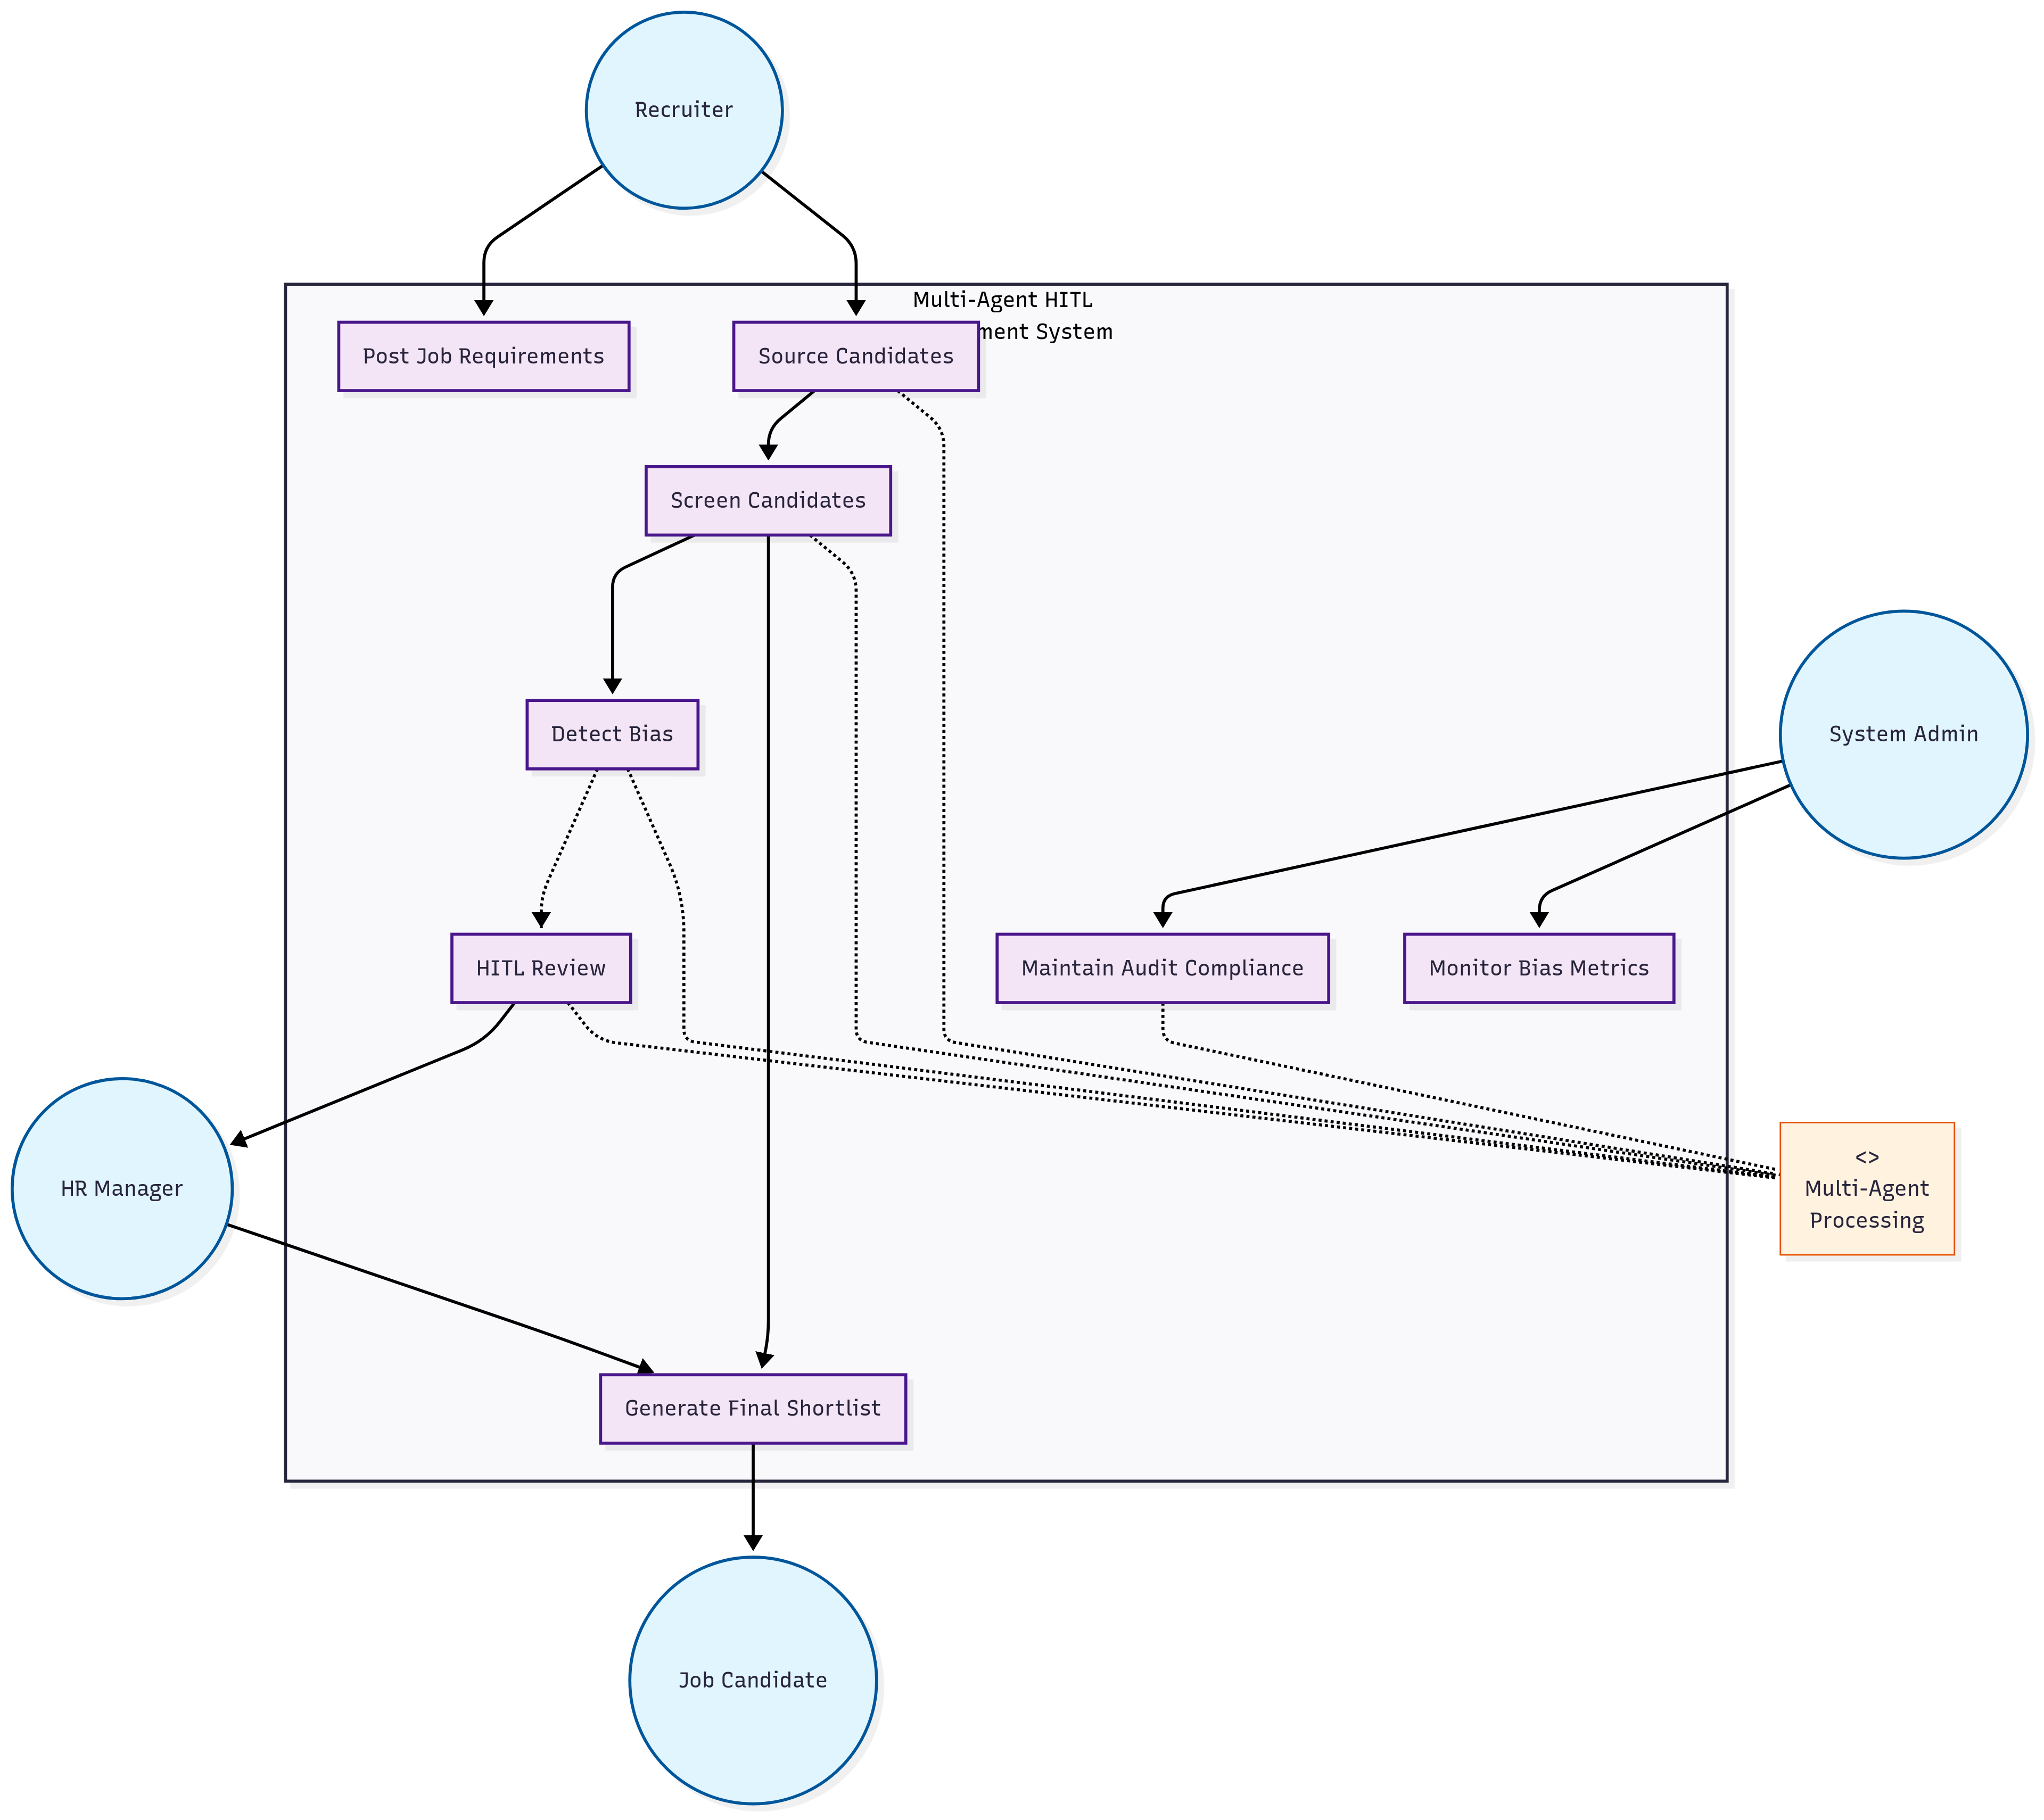
\includegraphics[width=0.9\linewidth]{img/recruitment-system-mas.png}
    \caption{\textit{Quy trình vận hành hệ thống tuyển}}
    \label{fig:recruitment-system-mas}
\end{figure}

Quy trình vận hành tổng thể của hệ thống được minh hoạ chi tiết tại \hyperref[fig:recruitment-system-mas]{\color{blue}{Hình 4.1}}, mô tả một chu trình khép kín, tích hợp chặt chẽ giữa các tác nhân tự động và sự giám sát của con người. Luồng hoạt động khởi đầu khi \textbf{Nhà tuyển dụng (Recruiter)} đăng tải các \textbf{Yêu cầu Công việc (Post Job Requirements)}. Ngay sau đó, Hệ thống Đa tác nhân (MAS) tiếp nhận và thực hiện một chuỗi các tác vụ tự động, bao gồm \textbf{Tìm kiếm ứng viên (Source Candidates)}, \textbf{Sàng lọc ứng viên (Screen Candidates)}, và \textbf{Phát hiện thiên vị (Detect Bias)}.

Dựa trên kết quả sàng lọc sơ bộ, hệ thống sẽ phân luồng xử lý. Các hồ sơ ứng viên rõ ràng, đạt độ tin cậy cao sẽ được hệ thống xử lý để \textbf{Tạo danh sách rút gọn cuối cùng (Generate Final Shortlist)}. Ngược lại, những trường hợp phức tạp, có độ tin cậy thấp, hoặc bị gắn cờ cảnh báo thiên vị sẽ được tự động chuyển đến quy trình \textbf{Đánh giá HITL (HITL Review)}. Tại bước này, \textbf{Trưởng phòng Nhân sự (HR Manager)} sẽ trực tiếp xem xét, đánh giá và đưa ra quyết định cuối cùng. Quyết định này không chỉ giải quyết các trường hợp cụ thể mà còn được ghi nhận và sử dụng làm dữ liệu phản hồi, tạo thành một vòng lặp cải tiến liên tục cho các mô hình của MAS. Song song với quy trình tuyển dụng chính, \textbf{Quản trị viên Hệ thống (System Admin)} thực hiện vai trò giám sát liên tục, bao gồm việc \textbf{Duy trì tuân thủ kiểm toán (Maintain Audit Compliance)} và \textbf{Theo dõi các chỉ số thiên vị (Monitor Bias Metrics)}, nhằm đảm bảo hệ thống vận hành một cách ổn định, minh bạch và công bằng.

\subsubsection{Các kịch bản vận hành chính}
Để minh họa rõ hơn luồng hoạt động của hệ thống, mục này sẽ mô tả chi tiết các kịch bản vận hành chính và các kịch bản hỗ trợ. Các kịch bản này làm rõ cách hệ thống cân bằng giữa quy trình xử lý tự động và sự can thiệp cần thiết của con người, đảm bảo tính hiệu quả và công bằng.

\paragraph{Kịch Bản Chính}

\begin{longtable}{|
  >{\raggedright\arraybackslash}p{0.08\textwidth}|
  >{\raggedright\arraybackslash}p{0.14\textwidth}|
  >{\raggedright\arraybackslash}p{0.12\textwidth}|
  >{\raggedright\arraybackslash}p{0.18\textwidth}|
  >{\raggedright\arraybackslash}p{0.14\textwidth}|
  >{\raggedright\arraybackslash}p{0.26\textwidth}|}

  \hline
  \textbf{Mã} &
  \textbf{Kịch bản} &
  \textbf{Tác nhân} &
  \textbf{Điều kiện đầu vào} &
  \textbf{Kết quả} &
  \textbf{Các bước chính (rút gọn)} \\
  \hline
  \endfirsthead

  % No header on continuation pages
  \endhead

  \hline
  \endfoot

  \hline
  \caption{\textit{Các Kịch Bản Chính}} \\
  \endlastfoot

  UC-OP-01 &
  Sàng lọc tự động tiêu chuẩn &
  Hệ thống &
  Đã có vị trí tuyển dụng và danh sách ứng viên &
  Khoảng 70–80\% hồ sơ được xử lý tự động &
  1. Truy xuất hồ sơ → 2. So khớp tiêu chí → 3. Phát hiện thiên vị → 4. Chấm điểm → 5. Chuyển bước → 6. Thông báo → 7. Ghi log \\
  \hline

  UC-OP-02 &
  HITL cho các trường hợp đặc biệt &
  Trưởng phòng nhân sự &
  Mức độ tin cậy < 0.7 hoặc có thiên vị &
  Có can thiệp người; mô hình được điều chỉnh &
  1. Chuyển tiếp → 2. Trình bày bằng chứng → 3. Trao đổi → 4. Quyết định → 5. Cập nhật mô hình → 6. Thông báo \\
  \hline

  UC-OP-03 &
  Phát hiện \& khắc phục thiên vị &
  Quản trị viên &
  Vi phạm chỉ số công bằng &
  Khắc phục thiên vị; được ghi nhận tuân thủ &
  1. Nhận diện mẫu → 2. Thông báo bên liên quan → 3. Phân tích hồ sơ → 4. Sửa đổi → 5. Đánh giá lại → 6. Báo cáo \\
\end{longtable}
\paragraph{Kịch Bản Hỗ Trợ}

\begin{longtable}{|
  >{\raggedright\arraybackslash}p{0.08\textwidth}|
  >{\raggedright\arraybackslash}p{0.18\textwidth}|
  >{\raggedright\arraybackslash}p{0.12\textwidth}|
  >{\raggedright\arraybackslash}p{0.18\textwidth}|
  >{\raggedright\arraybackslash}p{0.14\textwidth}|
  >{\raggedright\arraybackslash}p{0.25\textwidth}|}

  \hline
  \textbf{Mã} &
  \textbf{Kịch bản} &
  \textbf{Tác nhân} &
  \textbf{Điều kiện đầu vào} &
  \textbf{Kết quả} &
  \textbf{Các bước chính (rút gọn)} \\
  \hline
  \endfirsthead

  % No header on continuation pages
  \endhead

  \hline
  \endfoot

  \hline
  \caption{\textit{Các Kịch Bản Hỗ Trợ}} \\
  \endlastfoot

  UC-OP-04 &
  Thêm ứng viên thủ công &
  Nhà tuyển dụng &
  Đang có bài đăng tuyển &
  Ứng viên được đưa vào quy trình tiêu chuẩn &
  Thêm ứng viên → Xác minh → Ghi chú → Gửi đến sàng lọc \\
  \hline

  UC-OP-05 &
  Trao đổi đa vòng trong HITL &
  Trưởng phòng nhân sự &
  Hồ sơ bị gắn cờ; thiếu ngữ cảnh rõ ràng &
  Vấn đề được giải quyết; thông tin được học tập &
  Xem xét → Yêu cầu bổ sung → Trao đổi → Quyết định → Ghi nhận \\
\end{longtable}

\paragraph{Quy Trình Đánh Giá HITL}
\begin{figure}[H]
    \centering
    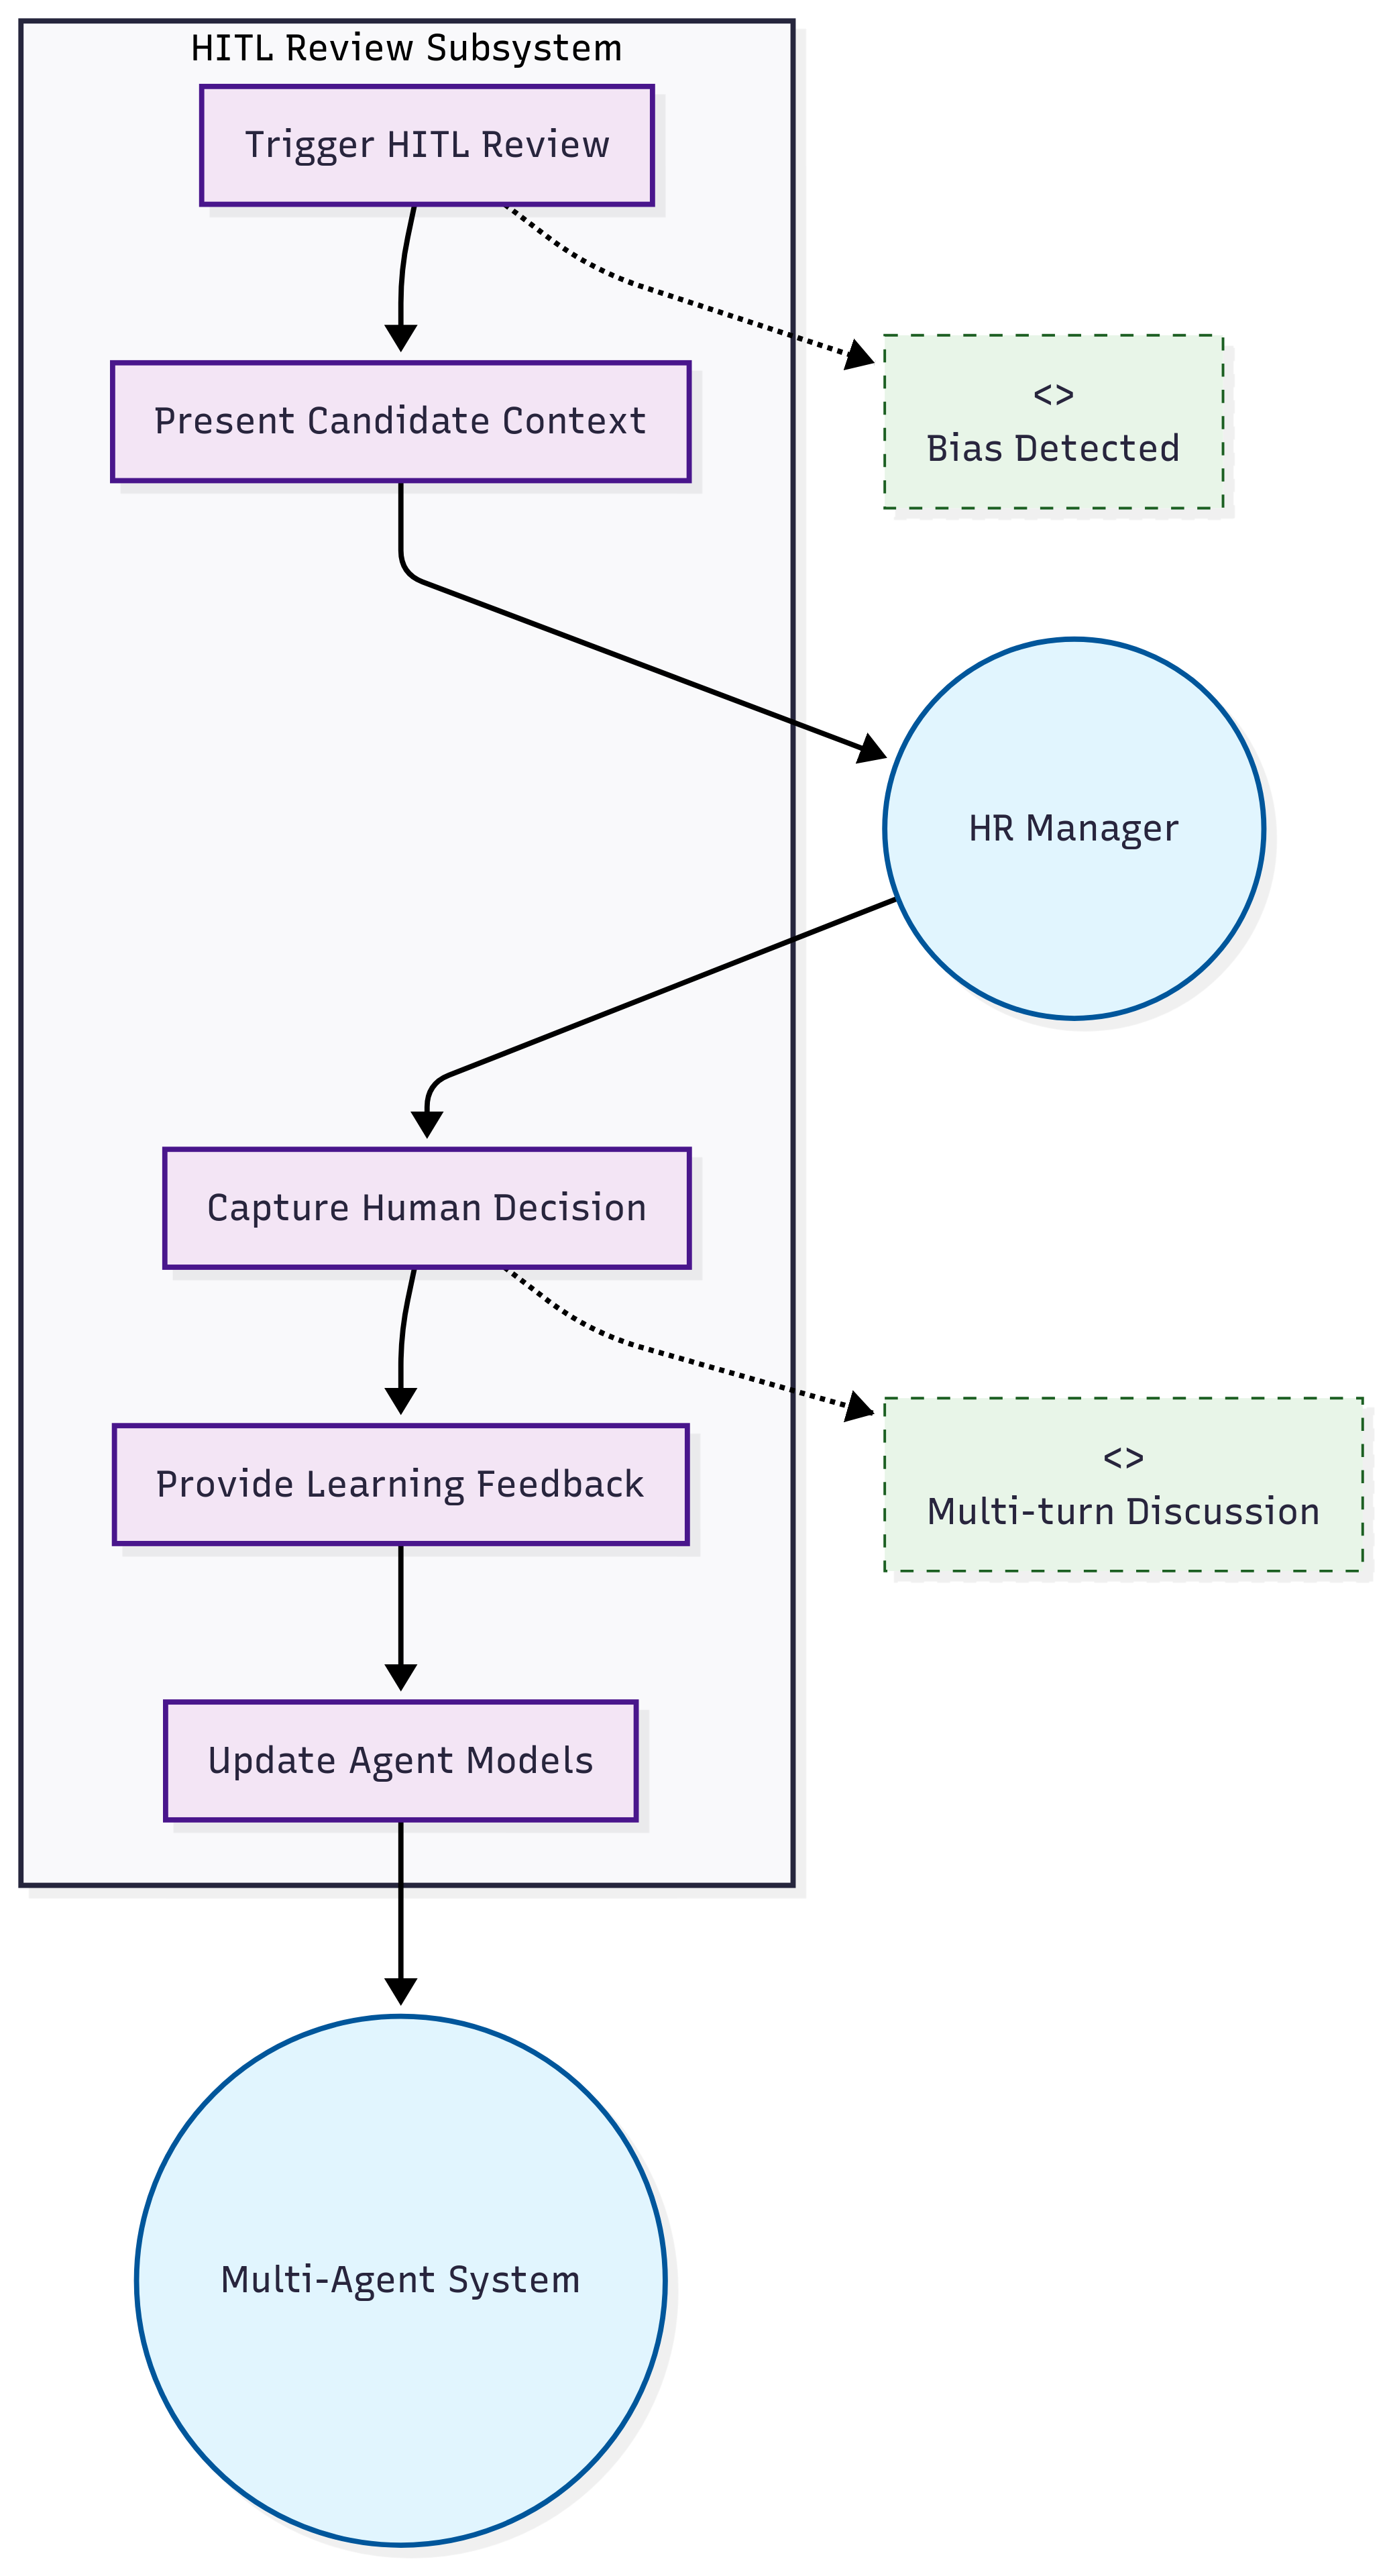
\includegraphics[width=0.5\linewidth]{img/hitl-review.png}
    \caption{\textit{Quy trình đánh giá HITL}}
    \label{fig:hitl-review}
\end{figure}

Quy trình Đánh giá có Con người trong Vòng lặp (HITL) là một tiểu hệ thống được thiết kế có cấu trúc, kích hoạt khi hệ thống tự động gặp phải một trường hợp có độ tin cậy thấp hoặc phát hiện dấu hiệu thiên vị (kịch bản UC-OP-02). Như được minh họa trong \hyperref[fig:hitl-review]{\color{blue}{Hình 4.2}}, luồng xử lý bắt đầu khi tiểu hệ thống HITL được khởi tạo. Hệ thống sẽ tiến hành \textbf{Trình bày Bối cảnh Ứng viên (Present Candidate Context)} một cách đầy đủ cho \textbf{Trưởng phòng Nhân sự (HR Manager)}. Bối cảnh này bao gồm các thông tin liên quan và đặc biệt là các cảnh báo về \textbf{Thiên vị được phát hiện (Bias Detected)}, nhằm cung cấp một góc nhìn toàn diện để hỗ trợ việc ra quyết định.

Sau khi xem xét các bằng chứng, quyết định của Trưởng phòng Nhân sự sẽ được hệ thống \textbf{Ghi nhận (Capture Human Decision)}. Điểm cốt lõi của quy trình này là quyết định của con người không chỉ để giải quyết trường hợp riêng lẻ mà còn được chuyển đổi thành \textbf{Phản hồi học tập (Provide Learning Feedback)}. Tín hiệu phản hồi này sau đó được sử dụng để \textbf{Cập nhật các Mô hình Tác nhân (Update Agent Models)}, tạo ra một chu trình cải tiến liên tục. Thông qua cơ chế này, Hệ thống Đa tác nhân (Multi-Agent System) có khả năng học hỏi từ kinh nghiệm và phán đoán của chuyên gia, từ đó nâng cao độ chính xác và giảm thiểu các sai sót tương tự trong các chu kỳ tuyển dụng tiếp theo.

\subsection{Mô tả hệ thống đa tác nhân}
Để hiện thực hóa các yêu cầu đã đề ra, luận văn đề xuất một kiến trúc đa tác nhân (MAS) dạng mô-đun, trong đó các chức năng được phân bổ cho các tác nhân phần mềm chuyên biệt. Các tác nhân này phối hợp chặt chẽ với nhau theo một quy trình được điều phối tập trung, nhằm chuyển đổi mô tả công việc và dữ liệu ứng viên thô thành một danh sách rút gọn được xếp hạng, có khả năng giải thích, giảm thiểu thiên vị và tuân thủ các tiêu chuẩn kiểm toán. Mỗi tác nhân vận hành trên một cấu trúc dữ liệu chung và giao thức thống nhất, đảm bảo quá trình xử lý diễn ra minh bạch và mọi quyết định đều có thể được kiểm chứng.

\subsubsection{Sơ đồ Kiến trúc Hệ thống}
Kiến trúc tổng thể của hệ thống được minh họa chi tiết trong hình bên dưới. Sơ đồ này thể hiện một cách chi tiết kiến trúc tổng thể của hệ thống đa tác nhân được đề xuất, làm rõ luồng dữ liệu, sự tương tác giữa các thành phần và vai trò của từng lớp chức năng. Kiến trúc này được thiết kế theo một mô hình khép kín, nơi con người và các tác nhân AI phối hợp chặt chẽ để thực hiện quy trình tuyển dụng một cách thông minh và có khả năng tự cải tiến.

\begin{figure}[H]
    \centering
    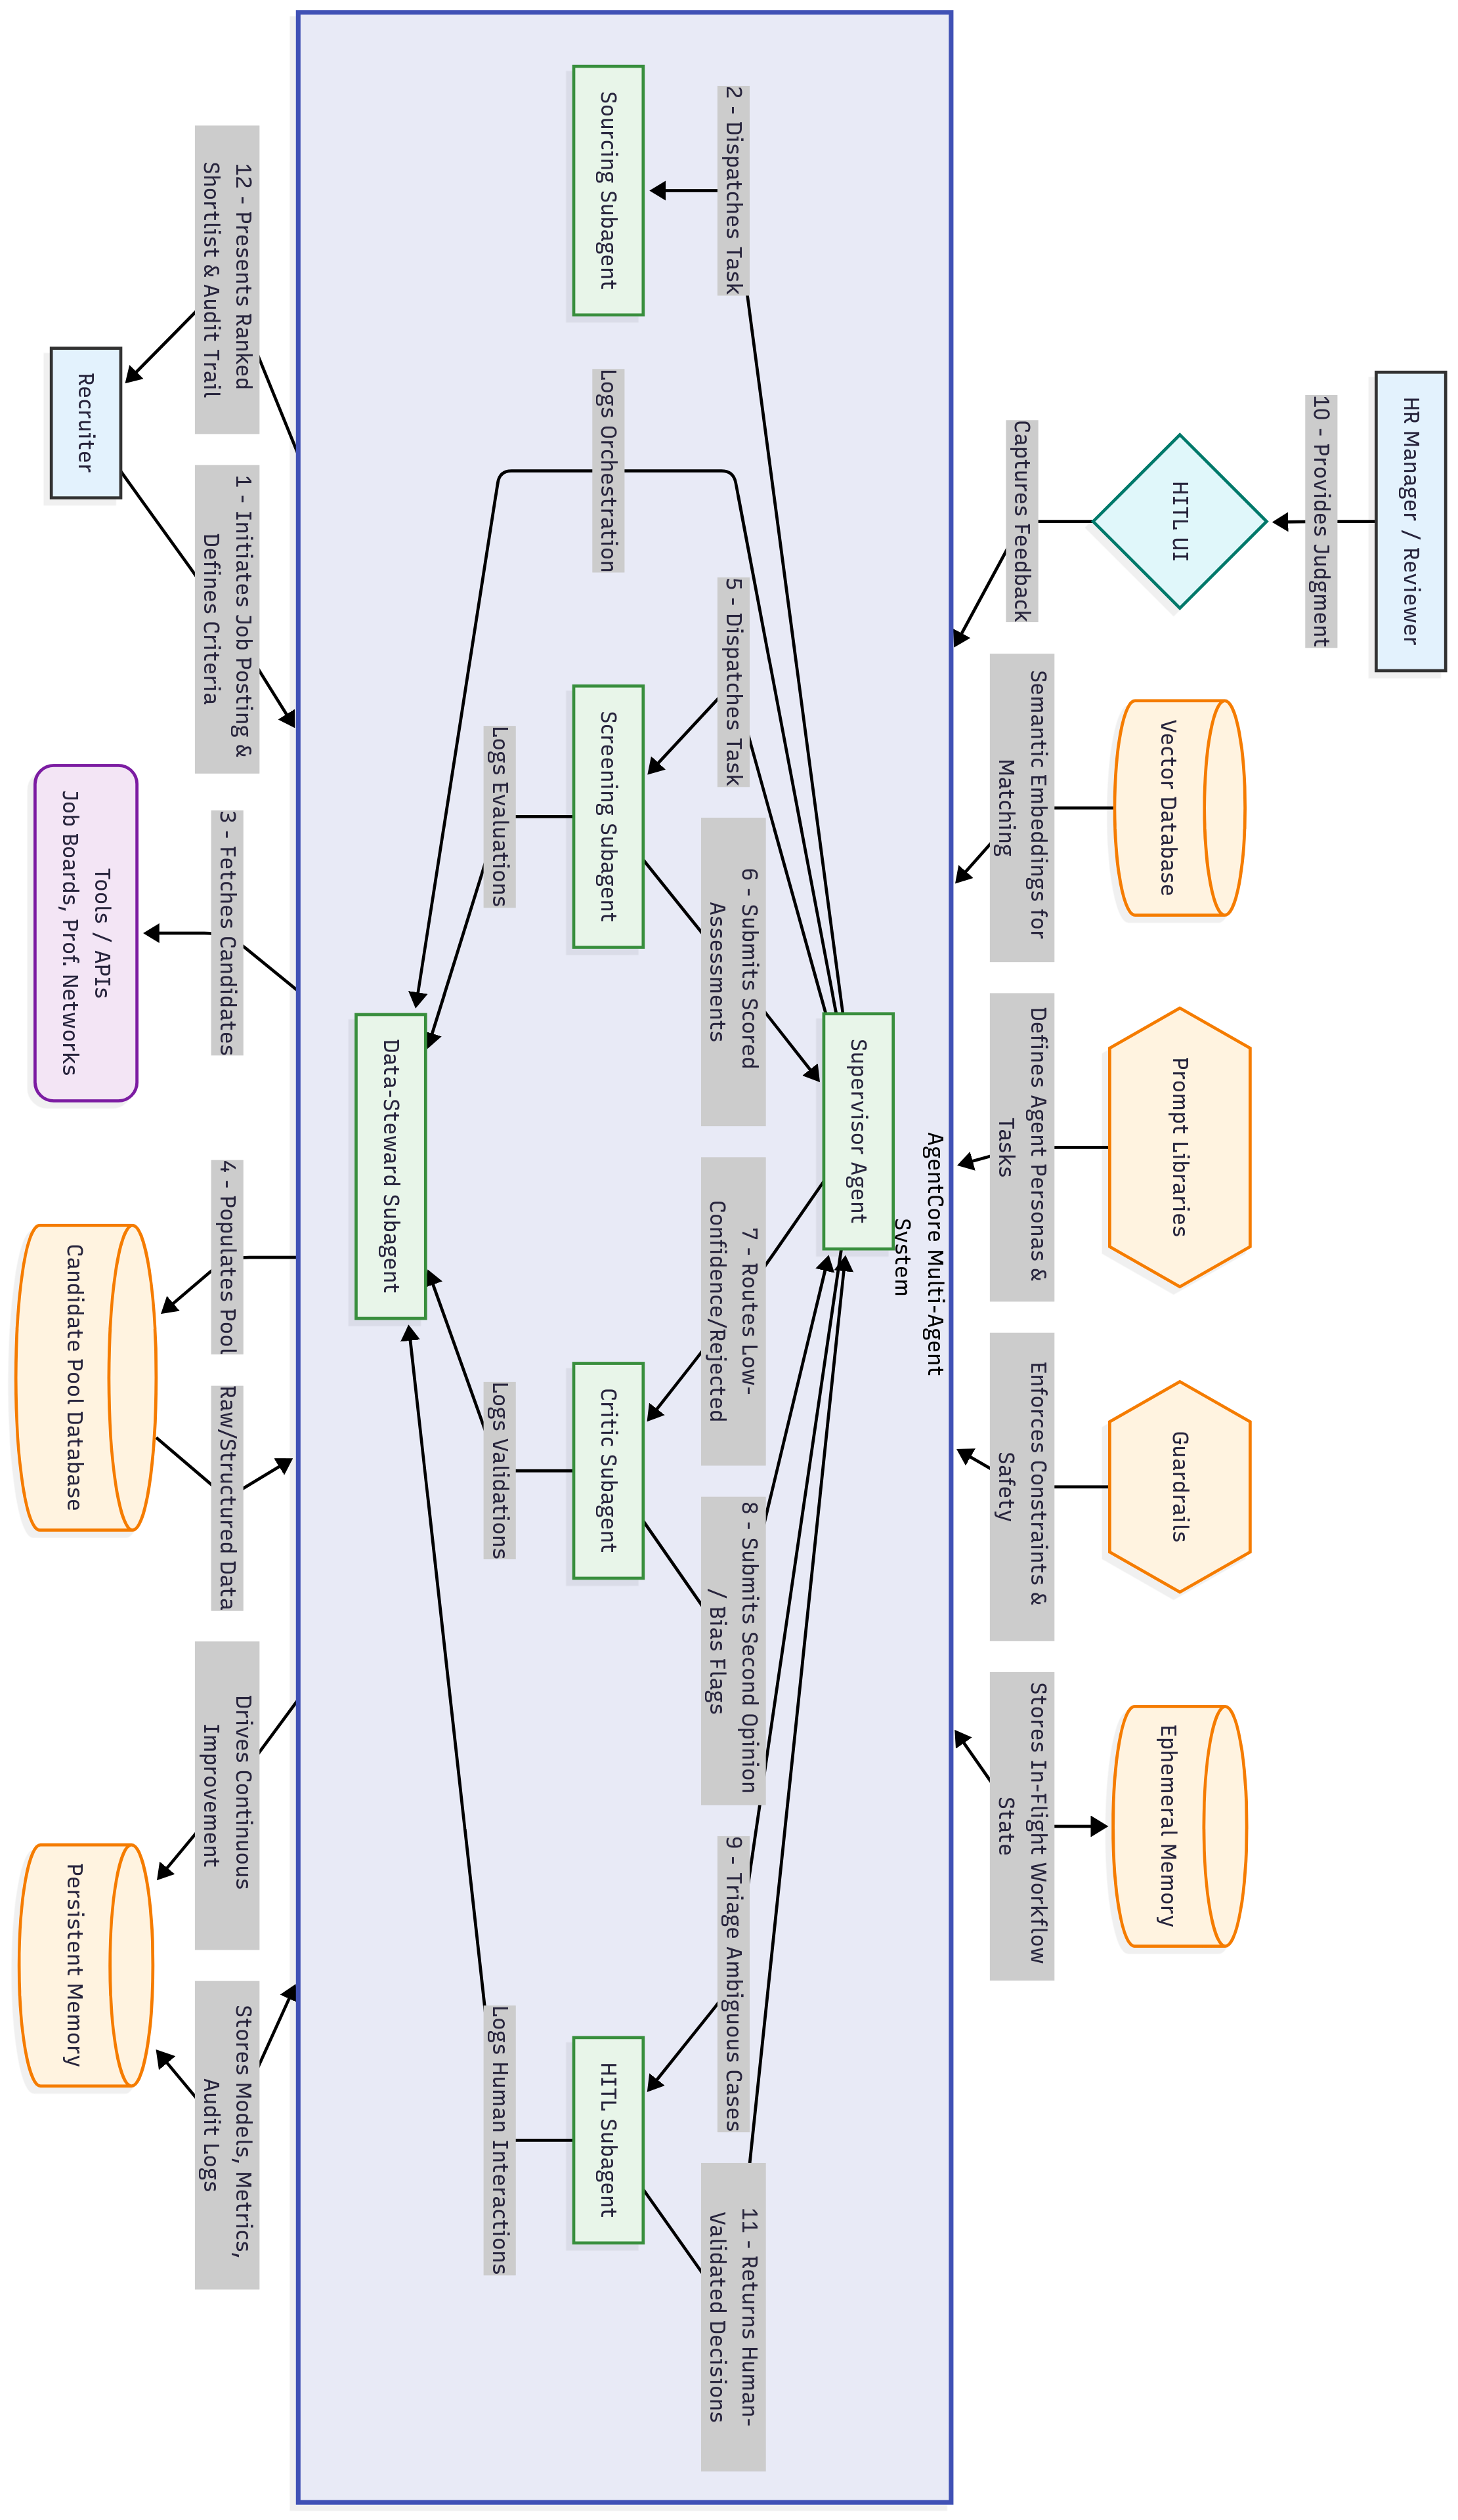
\includegraphics[width=0.85\linewidth]{img/architecture-diagram.png}
    \caption{\textit{Kiến trúc cốt lõi của hệ thống đa tác nhân}}
    \label{fig:architecture-diagram}
\end{figure}

Ngay trung tâm của hình (trong hộp màu xanh lớn) là \textbf{AgentCore Multi-Agent System}, đóng vai trò là bộ não xử lý của toàn bộ kiến trúc. Lõi của hệ thống này là một Supervisor Agent (Tác nhân Giám sát) có chức năng điều phối và phân luồng nhiệm vụ. Nó tương tác với một tập hợp các Subagents (Tác nhân phụ) chuyên biệt để thực hiện các công đoạn khác nhau của quy trình tuyển dụng. Các tác nhân phụ này bao gồm:
\begin{itemize}[topsep=0pt, itemsep=4pt, leftmargin=40pt]
    \item \textbf{Sourcing Subagent} (Tác nhân Tìm kiếm): Chịu trách nhiệm thu thập dữ liệu ứng viên.
    \item \textbf{Screening Subagent} (Tác nhân Sàng lọc): Đánh giá và chấm điểm hồ sơ.
    \item \textbf{Critic Subagent} (Tác nhân Phản biện): Đưa ra một góc nhìn thứ hai để kiểm tra thiên vị và phát hiện tiềm năng ẩn.
    \item \textbf{HITL Subagent} (Tác nhân có Con người trong Vòng lặp): Quản lý sự tương tác và nhận phán quyết từ con người.
    \item \textbf{Data-Steward Subagent} (Tác nhân Quản lý Dữ liệu): Ghi nhận và lưu trữ toàn bộ các tương tác, quyết định và dữ liệu để đảm bảo tính minh bạch và khả năng kiểm toán.
\end{enumerate}

Bên trái của sơ đồ là các tác nhân con người và các nguồn dữ liệu bên ngoài. Quy trình được khởi tạo (1) bởi \textbf{Recruiter} (Nhà tuyển dụng), người định nghĩa các tiêu chí công việc. \textbf{Sourcing Subagent} sau đó sẽ thực hiện nhiệm vụ được giao (2) bằng cách tìm kiếm và lấy dữ liệu ứng viên (3) từ các nguồn bên ngoài như \textbf{Tools / APIs} (các trang tuyển dụng, mạng lưới chuyên nghiệp). Dữ liệu thô này sau đó được điền vào (4) \textbf{Candidate Pool Database} (Cơ sở dữ liệu hồ sơ ứng viên).

Bên phải của sơ đồ là các thành phần hạ tầng hỗ trợ cho AgentCore. \textbf{Supervisor Agent} sử dụng \textbf{Prompt Libraries} (Thư viện mẫu) để định nghĩa vai trò và tác vụ cho các tác nhân, dùng \textbf{Vector Database} (Cơ sở dữ liệu vector) cho việc so khớp ngữ nghĩa, áp dụng các \textbf{Guardrails} (Rào cản) để đảm bảo an toàn và tuân thủ, và sử dụng \textbf{Ephemeral Memory} (Bộ nhớ tạm thời) để lưu trữ trạng thái của các quy trình đang diễn ra. Dữ liệu mang tính chiến lược như các mô hình đã huấn luyện, các số liệu hiệu suất và nhật ký kiểm toán được lưu trữ trong \textbf{Persistent Memory} (Bộ nhớ lâu dài).

Luồng xử lý dữ liệu được điều phối một cách chặt chẽ. Sau khi có dữ liệu ứng viên, \textbf{Supervisor Agent} sẽ giao nhiệm vụ sàng lọc (5) cho \textbf{Screening Subagent}. Tác nhân này sẽ gửi lại kết quả đánh giá đã chấm điểm (6). Dựa trên độ tin cậy của kết quả, \textbf{Supervisor Agent} có thể định tuyến các trường hợp có độ tin cậy thấp hoặc bị từ chối (7) đến \textbf{Critic Subagent} để nhận một "ý kiến thứ hai" và các cảnh báo về thiên vị (8). Các trường hợp phức tạp hoặc không rõ ràng sẽ được phân loại và chuyển (9) đến \textbf{HITL Subagent}. Tại đây, thông qua \textbf{HITL UI} (Giao diện người dùng), \textbf{HR Manager / Reviewer} (Trưởng phòng Nhân sự / Người đánh giá) sẽ đưa ra phán quyết cuối cùng (10). Quyết định đã được xác thực bởi con người này sau đó được trả về hệ thống (11).

Xuyên suốt quy trình, \textbf{Data-Steward Subagent} đóng vai trò quan sát và ghi nhận toàn bộ hoạt động, bao gồm việc điều phối, các kết quả đánh giá, các kết quả xác thực và các tương tác của con người, tạo ra một dòng chảy dữ liệu nhất quán và có thể truy vết. Cuối cùng, hệ thống sẽ trình bày một danh sách ứng viên đã được xếp hạng cùng với toàn bộ nhật ký kiểm toán (12) cho \textbf{Recruiter}, hoàn tất một chu trình khép kín, minh bạch và thông minh.

\paragraph{Hạ tầng nền tảng và kiến trúc bộ nhớ}
Để hỗ trợ kiến trúc phân tán này, các tác nhân vận hành trên một \textbf{hạ tầng nền tảng (AgentCore)}. AgentCore cung cấp các dịch vụ dùng chung thiết yếu như quản lý trạng thái, thực thi an toàn trong môi trường biệt lập (sandboxing) và giao tiếp, tương tự vai trò của các nền tảng điều phối container hiện đại như Kubernetes.

Một thành phần quan trọng của hạ tầng này là \textbf{kiến trúc bộ nhớ đa tầng (multi-tiered memory)}, được tối ưu cho từng mục đích sử dụng riêng biệt:
\begin{itemize}[topsep=0pt, itemsep=4pt, leftmargin=40pt]
    \item \textbf{Bộ nhớ tạm thời (Ephemeral Memory)}: Lưu trữ trạng thái của các quy trình và hội thoại đang diễn ra, và sẽ được giải phóng sau khi chu trình hoàn tất.
    \item \textbf{Cơ sở dữ liệu Ứng viên và Vector}: Lưu trữ hồ sơ đã được chuẩn hóa và các biểu diễn ngữ nghĩa (embeddings) của chúng để phục vụ cho việc so khớp và tìm kiếm tốc độ cao.
    \item \textbf{Bộ nhớ lâu dài (Persistent Memory)}: Lưu trữ các dữ liệu mang tính chiến lược như nhật ký kiểm toán, các chỉ số hiệu suất, phân tích thiên vị và các mô hình AI đã được huấn luyện lại.
\end{itemize}

Sự phân tầng này đảm bảo dữ liệu luôn phù hợp với ngữ cảnh, dễ truy xuất, và đáp ứng được cả yêu cầu về hiệu năng thời gian thực lẫn lưu trữ dài hạn. Nhìn chung, các quyết định thiết kế—từ giao tiếp bất đồng bộ, điều phối tập trung, đến lưu trữ đa hình (polyglot persistence)—cùng nhau tạo nên một hệ thống không chỉ hiệu quả về mặt tính toán mà còn mạnh mẽ về khả năng chịu lỗi, dễ bảo trì và sẵn sàng cho việc mở rộng trong tương lai.


\subsubsection{Đặc tả tác nhân phụ}
Hệ thống được đề xuất vận hành dựa trên một kiến trúc đa tác nhân (MAS) dạng mô-đun, trong đó sáu tác nhân phụ chuyên biệt phối hợp chặt chẽ với nhau (minh họa trong \hyperref[fig:architecture-diagram]{\color{blue}{Hình 4.3}}). Các tác nhân này cùng thực hiện một quy trình thống nhất nhằm chuyển đổi các mô tả công việc và hồ sơ ứng viên từ dạng thô, không đồng nhất thành một danh sách rút gọn cuối cùng. Kết quả trả về là một danh sách được xếp hạng, có khả năng giải trình minh bạch, đã được kiểm tra và giảm thiểu thiên vị, đồng thời tuân thủ các tiêu chuẩn kiểm toán và pháp lý. Mỗi tác nhân đảm nhận một chức năng hẹp nhưng vận hành trên một cấu trúc dữ liệu và giao thức chung, đảm bảo quá trình chuyển giao nhiệm vụ diễn ra liền mạch và mọi quyết định đều có thể được kiểm chứng.

\paragraph{a. Tác nhân giám sát (Orchestrator)}

Đóng vai trò là trung tâm điều phối của hệ thống, Tác nhân Giám sát áp dụng mô hình "supervisor-router" để phân tách mô tả công việc thành một bộ tiêu chí đánh giá có cấu trúc và phân luồng nhiệm vụ cho các tác nhân chuyên biệt khác. Một chức năng quan trọng của nó là quản lý và điều tiết khối lượng công việc cho quy trình có con người can thiệp (Human-in-the-Loop - HITL), đảm bảo tỷ lệ hồ sơ cần chuyên gia xem xét luôn duy trì trong khoảng 15-25\%. Bằng cách này, hệ thống có thể tự động xử lý các trường hợp có độ tin cậy cao và chỉ chuyển những trường hợp phức tạp đến chuyên gia, tối ưu hóa hiệu suất toàn trình. Sau mỗi chu kỳ tuyển dụng, các trạng thái tạm thời sẽ được xóa, nhưng các số liệu về hiệu suất và thuật toán phân loại sẽ được lưu lại để liên tục cải thiện khả năng điều phối.

\paragraph{b. Tác nhân tìm kiếm ứng viên (Sourcing)}

Tác nhân Tìm kiếm hoạt động như một lớp thu thập dữ liệu đầu vào, chịu trách nhiệm tổng hợp và hợp nhất hồ sơ ứng viên từ nhiều nguồn khác nhau như API của các trang tuyển dụng, mạng lưới nghề nghiệp và cơ sở dữ liệu nội bộ. Sau khi thu thập, tác nhân này sẽ thực hiện các bước tiền xử lý cơ bản, bao gồm loại bỏ các hồ sơ trùng lặp và áp dụng bộ lọc điều kiện để sàng lọc nhanh những ứng viên rõ ràng không đủ tiêu chuẩn. Đầu ra của tác nhân là một tập hợp hồ sơ ứng viên đã được chuẩn hóa và làm giàu thông tin, sẵn sàng để chuyển sang giai đoạn đánh giá sâu hơn.

\paragraph{c. Tác nhân sàng lọc (Screening)}

Đây là tác nhân cốt lõi trong việc đánh giá chuyên môn. Nó có nhiệm vụ trích xuất các đặc trưng có cấu trúc từ hồ sơ ứng viên (résumé) và sử dụng mô hình đo lường tương đồng ngữ nghĩa để chấm điểm mức độ phù hợp giữa năng lực của ứng viên và yêu cầu công việc. Điểm đặc biệt của Tác nhân Sàng lọc là mỗi quyết định đánh giá đều đi kèm với một giải thích cụ thể, có khả năng truy vết, được dẫn chiếu trực tiếp từ những thông tin có trong hồ sơ ứng viên.

\paragraph{d. Tác nhân phản biện (Critic)}

Với vai trò là một cơ chế kiểm định độc lập, Tác nhân Phản biện đánh giá lại các ứng viên đã bị Tác nhân Sàng lọc loại bỏ. Mục tiêu của nó là phát hiện những tài năng tiềm ẩn có thể bị bỏ sót và chỉ ra các dấu hiệu của thiên vị hệ thống. Để làm được điều này, tác nhân sử dụng các phép ánh xạ khái niệm thay thế (ví dụ: xem xét kinh nghiệm "quản lý hậu cần trong quân đội" tương đương với "quản lý chuỗi cung ứng") để nhận diện năng lực của ứng viên theo một góc nhìn đa chiều hơn.

\paragraph{e. Tác nhân con người trong vòng lặp (HITL)}

Tác nhân này đóng vai trò là cầu nối giữa hệ thống tự động và chuyên gia tuyển dụng, được kích hoạt cho các trường hợp không chắc chắn hoặc có khả năng gây tranh cãi. Thông qua một giao diện đối thoại, nó trình bày đầy đủ bối cảnh và bằng chứng cho chuyên gia, đồng thời ghi nhận quyết định cuối cùng cùng với các chú thích về lý do. Những phản hồi này không chỉ giải quyết các trường hợp cụ thể mà còn được dùng làm dữ liệu huấn luyện quý giá để cải tiến hệ thống.

\paragraph{f. Tác nhân quản lý dữ liệu (Data-Steward)}

Tác nhân này đảm bảo các yếu tố về tuân thủ, minh bạch và cải tiến liên tục cho toàn hệ thống. Nó chịu trách nhiệm ẩn danh hóa các thông tin định danh cá nhân (PII), duy trì một nhật ký kiểm toán bất biến cho mọi quyết định, giám sát các chỉ số về tính công bằng, và tự động xây dựng các tập dữ liệu huấn luyện mới từ dữ liệu lịch sử. Tác nhân này có quyền truy cập đọc toàn bộ hệ thống nhưng quyền ghi được giới hạn nghiêm ngặt trong kho lưu trữ tuân thủ, đảm bảo tính toàn vẹn và bảo mật.

\subsubsection{Mô Hình Giao Tiếp}
Hạ tầng giao tiếp của hệ thống được xây dựng dựa trên kiến trúc phi đồng bộ, điều khiển bằng thông điệp (message-driven). Cách tiếp cận này tuân thủ bốn nguyên tắc thiết kế cốt lõi:
\begin{enumerate}[topsep=0pt, itemsep=4pt, leftmargin=40pt, label=\arabic*.]
    \item \textbf{Tách Biệt Tác Nhân}: Mỗi tác nhân vận hành với trạng thái riêng và chỉ trao đổi thông tin qua thông điệp, loại bỏ sự phụ thuộc vào bộ nhớ dùng chung. Điều này giúp khoanh vùng lỗi, hỗ trợ triển khai độc lập và tăng cường tính chịu lỗi của toàn hệ thống.
    \item \textbf{Ghi Nhận Nhật Ký Tập Trung}: Toàn bộ thông điệp được sao lưu tại Tác nhân Data-Steward. Việc tách riêng chức năng ghi nhận này giúp logic của từng tác nhân nghiệp vụ được tinh gọn, đồng thời đảm bảo khả năng kiểm tra và tuân thủ toàn diện.
    \item \textbf{Tích Hợp Phản Hồi Từ Con Người (HITL)}: Cơ chế giám sát và phản hồi từ người dùng tạo ra một nguồn dữ liệu huấn luyện chất lượng cao, có ngữ cảnh rõ ràng, giúp cải thiện liên tục các chính sách ra quyết định và thu hẹp khoảng cách giữa phán đoán của máy và chuyên gia.
    \item \textbf{Giao Tiếp Phi Đồng Bộ}: Việc sử dụng hàng đợi thông điệp (message broker) giúp tách biệt bên gửi và bên nhận, giảm nguy cơ tắc nghẽn, hỗ trợ khả năng mở rộng linh hoạt và tăng cường độ ổn định cho hệ thống.
\end{enumerate}

Tổng thể, các nguyên tắc này tạo nên một hạ tầng giao tiếp linh hoạt, có khả năng quan sát cao và thúc đẩy sự cải tiến liên tục thông qua các vòng phản hồi từ cả máy móc và con người.

\subsubsection{Quản lý Trạng thái Quy trình Tuyển dụng}
Để đảm bảo quá trình đánh giá ứng viên diễn ra một cách hiệu quả, minh bạch và có thể kiểm toán, hệ thống tích hợp một \textbf{Trình quản lý Trạng thái Quy trình (Workflow State Manager)}. Cơ chế này chuyển đổi quy trình tuyển dụng từ một luồng xử lý mờ thành một chuỗi các giai đoạn tuần tự, có liên kết chặt chẽ và được định danh bằng các trạng thái rõ ràng. Mỗi trạng thái đại diện cho một bước ra quyết định cụ thể, cho phép theo dõi chi tiết, truy vết lịch sử, và tạo ra một vòng lặp cải tiến liên tục cho hệ thống.

Luồng xử lý hồ sơ của một ứng viên sẽ đi qua sáu giai đoạn chính, tương ứng với sáu trạng thái cốt lõi sau:
\begin{enumerate}[topsep=0pt, itemsep=4pt, leftmargin=40pt, label=\arabic*.]
    \item \textbf{Khởi tạo (Initialization)}: Quy trình bắt đầu khi Tác nhân Giám sát phân tích một mô tả công việc và chuyển đổi nó thành một hồ sơ yêu cầu có cấu trúc, sẵn sàng cho việc so khớp. Trạng thái của quy trình lúc này là Job-Profile-Ready.
    \item \textbf{Sàng lọc Sơ bộ (Preliminary Screening)}: Dựa trên hồ sơ yêu cầu, hệ thống tiến hành sàng lọc song song trên toàn bộ danh sách ứng viên. Mỗi ứng viên sau đó sẽ được gán một điểm số ban đầu và chuyển sang trạng thái Screened-Preliminary.
    \item \textbf{Rà soát Thiên vị (Bias Audit)}: Ở giai đoạn này, Tác nhân Phản biện sẽ thực hiện một bước rà soát trọng yếu đối với các trường hợp được xem là ranh giới hoặc có nguy cơ bị bỏ sót. Mục tiêu là để kiểm tra các thiên vị tiềm ẩn và đánh giá lại năng lực. Sau khi hoàn tất, hồ sơ sẽ được chuyển sang trạng thái Bias-Audited.
    \item \textbf{Phân luồng Thông minh (Intelligent Triage)}: Hệ thống tính toán điểm tin cậy cho mỗi đánh giá và áp dụng các ngưỡng động để phân loại hồ sơ. Các trường hợp có độ tin cậy cao có thể được tự động xử lý, trong khi các trường hợp khác được phân luồng đến chuyên gia. Trạng thái lúc này là Triaged.
    \item \textbf{Hoàn tất Quyết định (Decision Finalization)}: Đối với các hồ sơ yêu cầu can thiệp, chuyên gia tuyển dụng sẽ xem xét bằng chứng và đưa ra quyết định cuối cùng. Sau khi quyết định của con người được ghi nhận, trạng thái của hồ sơ được cập nhật thành Decision-Finalised.
    \item \textbf{Học hỏi và Cập nhật (Model Update)}: Dữ liệu phản hồi từ các quyết định cuối cùng, đặc biệt là từ chuyên gia, sẽ được Tác nhân Quản trị viên thu thập. Dữ liệu này được dùng để huấn luyện lại và cải tiến các mô hình AI. Khi mô hình được làm mới, hệ thống chuyển sang trạng thái Model-Updated, hoàn tất một chu kỳ học hỏi.
\end{enumerate}

Mỗi một sự chuyển đổi giữa các trạng thái này đều được ghi nhận một cách nguyên tử vào sổ cái trạng thái của hệ thống. Điều này cho phép truy vết toàn bộ lịch sử xử lý của bất kỳ ứng viên nào, một yêu cầu thiết yếu cho việc kiểm toán và đánh giá tính công bằng. Đáng chú ý, việc tách biệt logic quản lý trạng thái khỏi logic nghiệp vụ của từng tác nhân giúp hệ thống có khả năng mở rộng cao. Các tác nhân mới—chẳng hạn như một bộ lọc hồ sơ nâng cao dùng NLP—có thể dễ dàng được tích hợp vào quy trình mà không làm ảnh hưởng đến khả năng truy xuất nguồn gốc. Cách tiếp cận này biến quy trình tuyển dụng thành một chuỗi vận hành công khai, có thể kiểm chứng và thích ứng linh hoạt với các nhu cầu của tổ chức.

\subsubsection{Cơ chế tương tác có con người trong vòng lặp (Human-in-the-Loop - HITL)}
Lớp tương tác có con người trong vòng lặp (HITL) là cơ chế kiểm soát chất lượng và đảm bảo tính công bằng cốt lõi của hệ thống. Thay vì yêu cầu chuyên gia tuyển dụng can thiệp vào mọi quyết định, quy trình HITL được thiết kế để kích hoạt một cách có chọn lọc, chỉ khi hệ thống có mức độ tự tin thấp hoặc khi phát hiện các trường hợp đặc biệt đã được định nghĩa trước. Cách tiếp cận này giúp cân bằng giữa hiệu suất xử lý tự động cho các hồ sơ rõ ràng và sự nhạy bén, sâu sắc trong phán đoán của con người đối với các trường hợp mơ hồ hoặc có nguy cơ bị đánh giá sai.

\paragraph{Nguyên tắc cốt lõi: Đánh giá dựa trên Độ đồng thuận}

Nền tảng của cơ chế HITL là việc tính toán một điểm tự tin (confidence score). Điểm này không dựa trên đánh giá của một tác nhân duy nhất, mà được xác định bởi mức độ đồng thuận giữa hai tác nhân độc lập với hai góc nhìn đối trọng:

\begin{enumerate}[topsep=0pt, itemsep=4pt, leftmargin=40pt, label=\arabic*.]
    \item \textbf{Tác nhân Sàng lọc (Screening Agent)}: Đánh giá mức độ phù hợp của ứng viên dựa trên các tiêu chí "truyền thống" và có cấu trúc, chẳng hạn như mức độ khớp về kỹ năng, kinh nghiệm làm việc, và bằng cấp liên quan.
    \item \textbf{Tác nhân Phản biện (Critic Agent)}: Cung cấp một góc nhìn bổ sung, tập trung vào các yếu tố thường bị các hệ thống ATS truyền thống bỏ qua như "tiềm năng và sự công bằng". Tác nhân này chủ động tìm kiếm các kỹ năng có thể chuyển đổi, phân tích hành trình phát triển của ứng viên, và phát hiện các dấu hiệu thiên vị hệ thống.
\end{enumerate}

Điểm tự tin của hệ thống được tính toán dựa trên độ chênh lệch tuyệt đối giữa điểm số của hai tác nhân ($s_{screen}$ và $s_{critic}$).
\begin{gather*}
\text{Confidence} = 1 - |s_{screen}-s_{critic}|
\end{gather*}

Nếu hai tác nhân hoàn toàn đồng thuận, điểm tự tin sẽ ở mức tối đa (là 1). Ngược lại, sự bất đồng quan điểm càng lớn thì điểm tự tin càng giảm, báo hiệu một trường hợp cần được con người xem xét cẩn trọng.

\paragraph{Phân luồng can thiệp đa cấp và các điều kiện đặc biệt}
\begin{figure}[H]
    \centering
    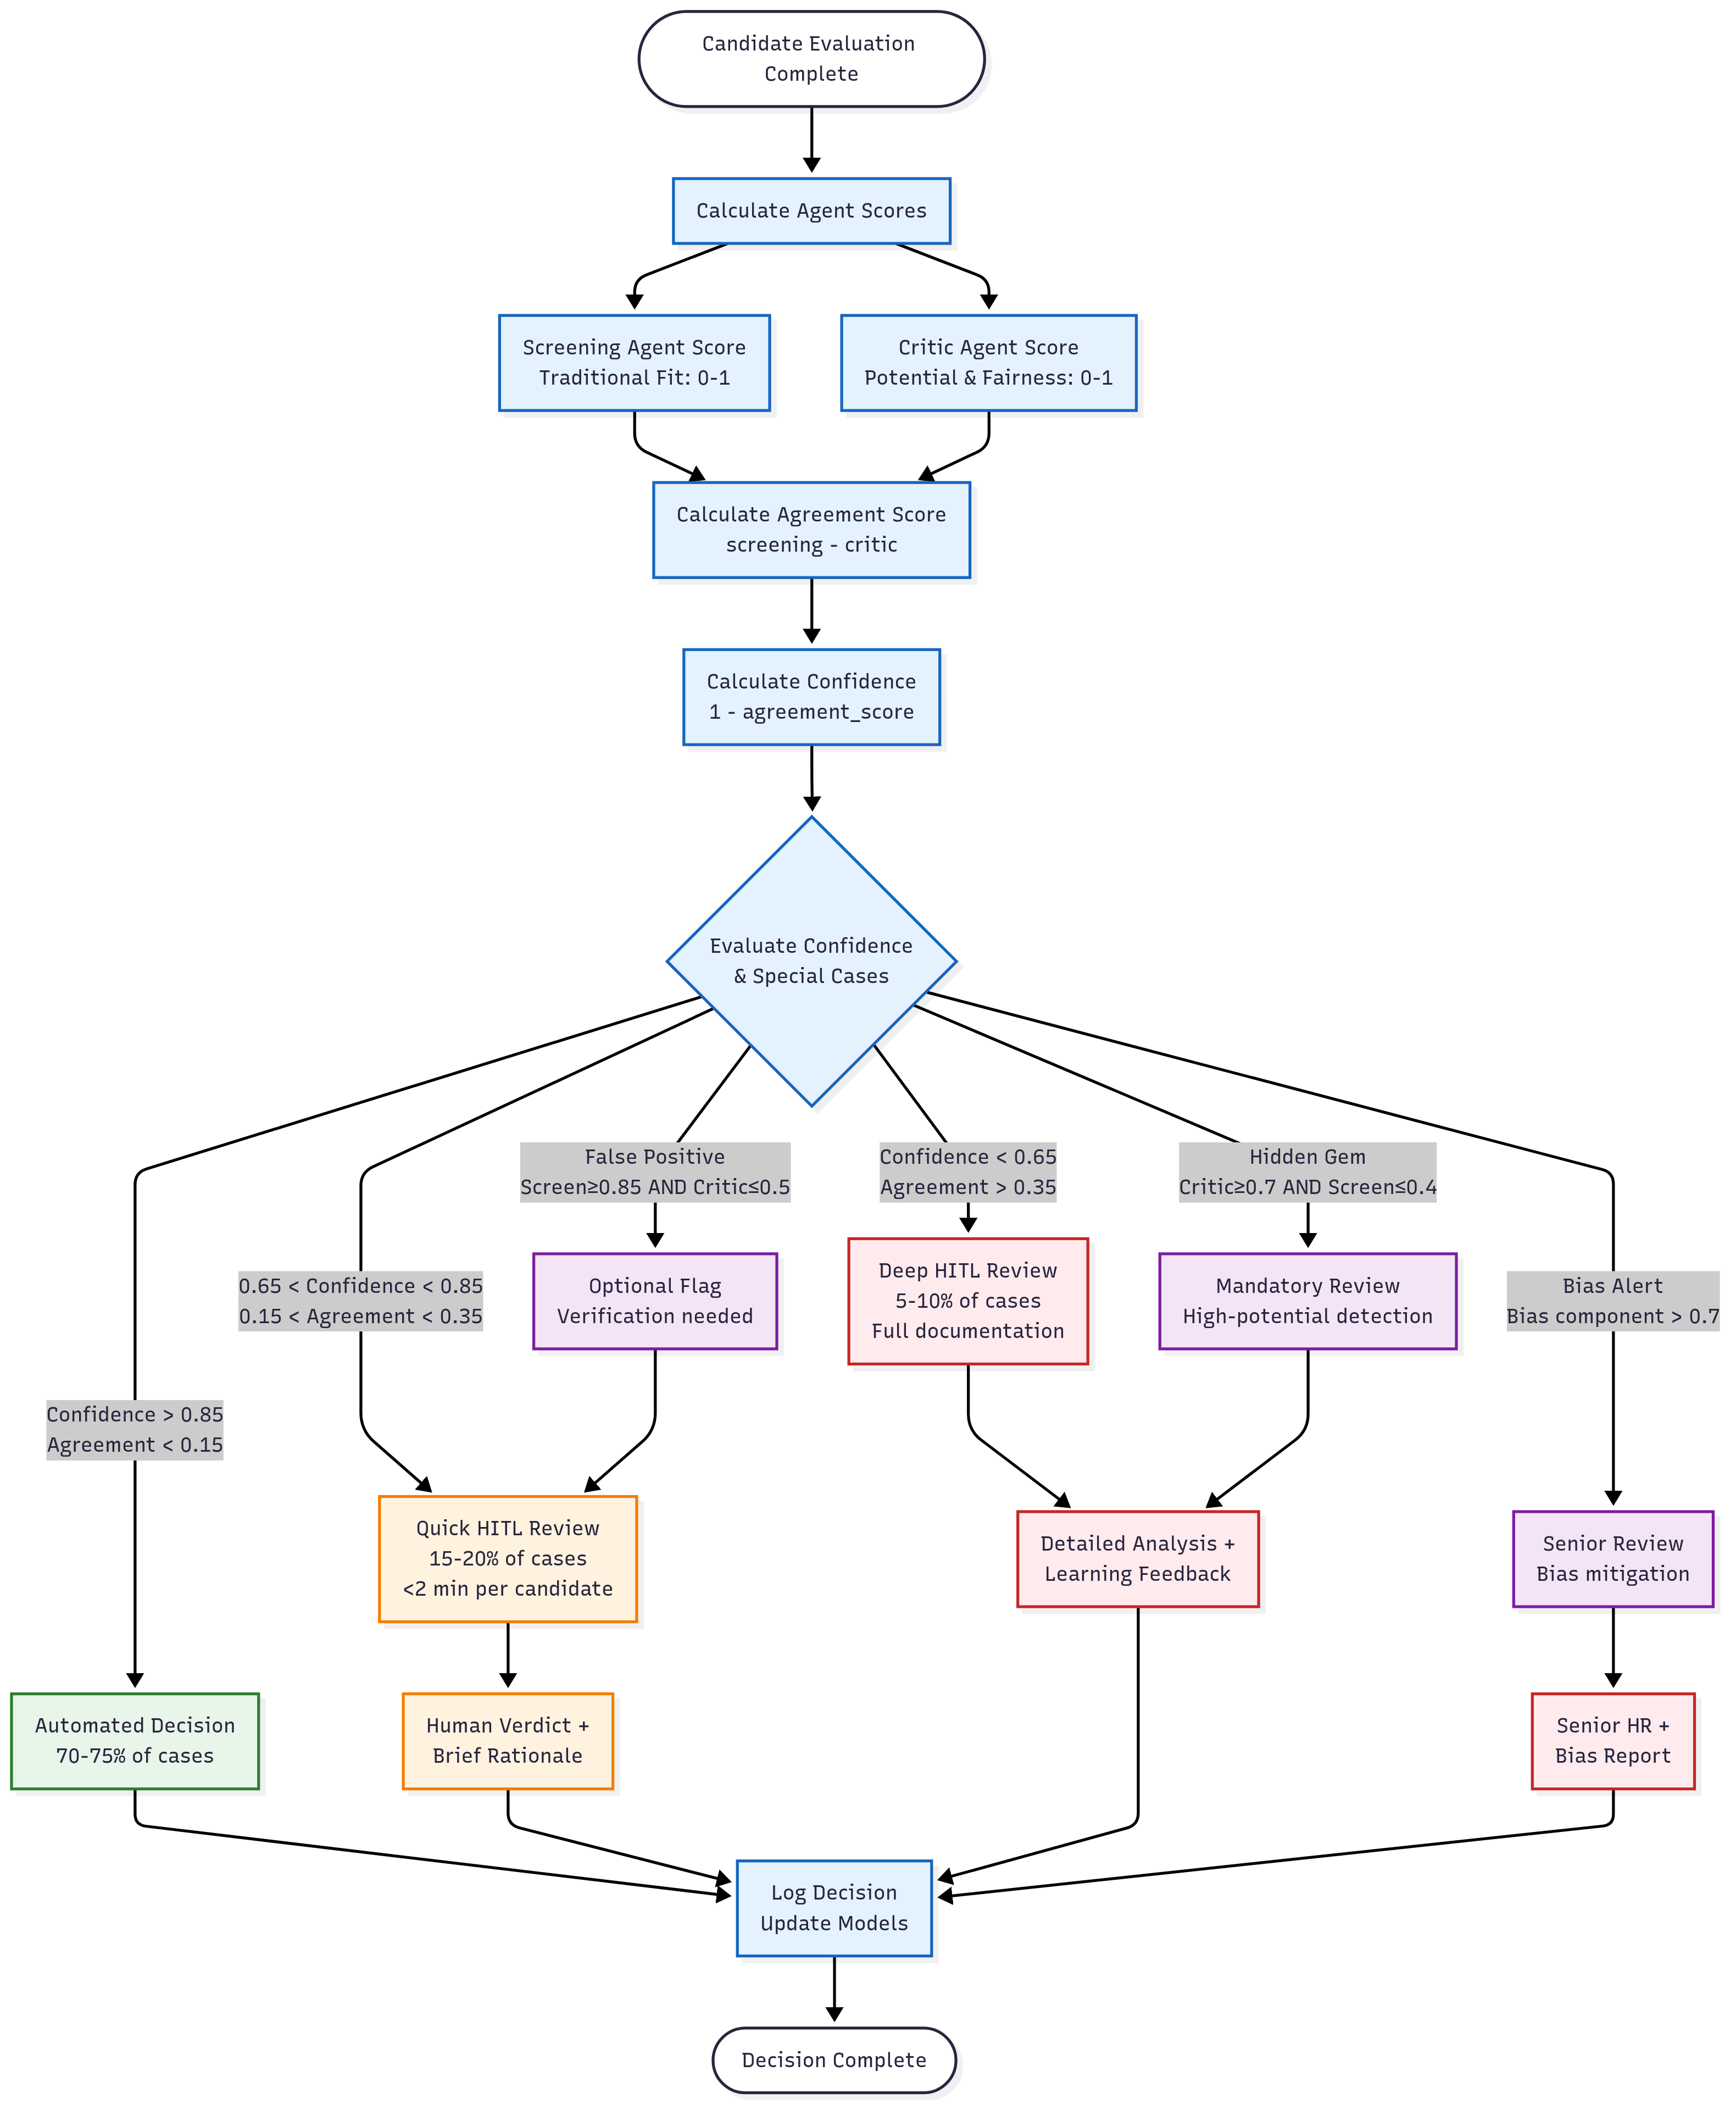
\includegraphics[width=0.9\linewidth]{img/hitl-decision-flow.png}
    \caption{\textit{Lưu đồ quyết định HITL}}
    \label{fig:hitl-decision-flow}
\end{figure}

\hyperref[fig:hitl-decision-flow]{\color{blue}{Hình 4.4}} minh họa chi tiết lưu đồ quyết định của cơ chế Tương tác có Con người trong Vòng lặp (HITL), thể hiện cách hệ thống phân luồng xử lý các trường hợp ứng viên một cách đa cấp dựa trên điểm tự tin và các điều kiện đặc biệt.

Quy trình bắt đầu sau khi \textbf{Tác nhân Sàng lọc} (Screening Agent) và \textbf{Tác nhân Phản biện} (Critic Agent) độc lập chấm điểm một ứng viên. Tác nhân Sàng lọc đánh giá dựa trên các tiêu chí truyền thống (Traditional Fit), trong khi Tác nhân Phản biện tập trung vào tiềm năng và sự công bằng (Potential & Fairness). Từ hai điểm số này, hệ thống tính toán một "Điểm đồng thuận" (Agreement Score) và một "Điểm tự tin" (Confidence Score) nghịch đảo với nó.

Dựa trên điểm tự tin, hệ thống sẽ tự động phân luồng xử lý theo một chiến lược đa cấp, được thể hiện trong lưu đồ trên.
\begin{itemize}[topsep=0pt, itemsep=4pt, leftmargin=40pt]
    \item \textbf{Tự động ra quyết định (Điểm tự tin > 0.85)}: Các trường hợp có độ đồng thuận cao (chiếm khoảng 70-75\% tổng số hồ sơ) sẽ được hệ thống tự động xử lý mà không cần can thiệp, giúp tối ưu hóa hiệu suất.
    \item \textbf{Duyệt nhanh (Quick Review) (0.65 < Điểm tự tin ≤ 0.85)}: Các trường hợp có sự chênh lệch vừa phải sẽ được chuyển đến chuyên gia cho một quy trình "duyệt nhanh", thường dưới 2 phút cho mỗi hồ sơ.
    \item \textbf{Xem xét toàn diện (Deep Review) (Điểm tự tin ≤ 0.65)}: Chỉ những trường hợp có sự bất đồng lớn nhất mới yêu cầu một cuộc xem xét thủ công toàn diện, với đầy đủ tài liệu và bối cảnh.
\end{itemize}

Ngoài ra, hệ thống cũng được lập trình để bắt buộc can thiệp thủ công trong một số \textbf{tình huống đặc biệt} nhằm tránh bỏ sót nhân tài hoặc các sai sót nghiêm trọng:
\begin{itemize}[topsep=0pt, itemsep=4pt, leftmargin=40pt]
    \item \textbf{Phát hiện "Viên ngọc ẩn" (Hidden Gem)}: Khi Tác nhân Phản biện chấm điểm rất cao ($s_{critic}\ge0.70$) cho một ứng viên mà Tác nhân Sàng lọc đã loại ($s_{screen} \le 0.40$).
    \item \textbf{Cảnh báo Thiên vị (Bias Alert)}: Khi thành phần đánh giá thiên vị của Tác nhân Phản biện vượt một ngưỡng nhất định, trường hợp sẽ được chuyển đến cấp quản lý cao hơn để xem xét.
    \item \textbf{Các trường hợp Ranh giới (Borderline Cases)}: Khi điểm số cuối cùng của ứng viên nằm trong khoảng ±5\% so với ngưỡng chấp nhận/loại.
\end{itemize}

Thông qua giao diện tương tác, chuyên gia có thể thực hiện nhiều hành động khác nhau tùy thuộc vào mức độ phức tạp của từng trường hợp, từ việc "duyệt/loại" nhanh, "chỉnh sửa/ghi chú" điểm số, tham gia vào một cuộc "trao đổi nhiều lượt" để làm rõ thông tin, cho đến "chuyển cấp xử lý" cho các hồ sơ đặc biệt nhạy cảm. Bằng cách kết hợp điểm tự tin, các quy tắc phát hiện thông minh và một quy trình đánh giá có cấu trúc, lớp HITL đảm bảo quá trình ra quyết định vừa hiệu quả về mặt thời gian, vừa công bằng và có trách nhiệm.

\subsection{Tổng kết chương}
Chương 4 đã trình bày một cách chi tiết và có hệ thống toàn bộ đặc tả kỹ thuật của hệ thống đa tác nhân, chuyển hóa các giải pháp lý thuyết đã được đề xuất ở chương trước thành một bản thiết kế kiến trúc cụ thể và khả thi. Mục tiêu xuyên suốt của chương là xây dựng một nền tảng vững chắc cho việc triển khai và kiểm nghiệm thực tế.

Nội dung chương khởi đầu bằng việc xác định các yêu cầu hệ thống một cách tường minh. Các yêu cầu chức năng được định nghĩa rõ ràng, tập trung vào các năng lực cốt lõi như phân tích ngữ nghĩa, phát hiện và giảm thiểu thiên vị, tạo giải thích cho quyết định, và tích hợp cơ chế có con người can thiệp (Human-in-the-Loop). Song song đó, các yêu cầu phi chức năng cũng được thiết lập chặt chẽ, bao gồm các tiêu chuẩn về hiệu năng, tính công bằng, bảo mật và khả năng vận hành, đảm bảo hệ thống không chỉ mạnh mẽ về mặt kỹ thuật mà còn đáng tin cậy và có trách nhiệm.

Trọng tâm của chương là phần mô tả kiến trúc đa tác nhân (MAS), một cấu trúc dạng mô-đun với sáu tác nhân chuyên biệt: \textbf{Giám sát (Orchestrator), Tìm kiếm (Sourcing), Sàng lọc (Screening), Phản biện (Critic), HITL, và Quản lý Dữ liệu (Data-Steward)}. Mỗi tác nhân đảm nhận một vai trò rõ ràng, phối hợp với nhau dưới sự điều phối của tác nhân Giám sát để xử lý hồ sơ ứng viên. Kiến trúc này được hỗ trợ bởi một hạ tầng giao tiếp phi đồng bộ và một hệ thống bộ nhớ đa tầng, giúp cô lập lỗi và tăng cường khả năng mở rộng. Toàn bộ quy trình vận hành, từ khi nhà tuyển dụng đăng tin đến khi hệ thống tạo ra danh sách ứng viên cuối cùng, được minh họa trực quan qua các sơ đồ luồng và tình huống sử dụng.

Điểm nổi bật trong thiết kế là cơ chế tương tác có con người trong vòng lặp (HITL) và hệ thống quản lý trạng thái quy trình. Quy trình HITL được kích hoạt một cách thông minh dựa trên "điểm tự tin", vốn được tính toán từ mức độ đồng thuận giữa hai tác nhân có góc nhìn đối trọng là Sàng lọc và Phản biện. Cách tiếp cận này giúp cân bằng tối ưu giữa hiệu suất xử lý tự động và sự giám sát sâu sắc của chuyên gia đối với các trường hợp phức tạp, đảm bảo chất lượng quyết định và tính công bằng. Cùng với đó, việc quản lý trạng thái theo từng giai đoạn rõ ràng giúp mọi bước xử lý trong quy trình đều trở nên minh bạch và có thể truy vết, đáp ứng các yêu cầu kiểm toán nghiêm ngặt.

Tóm lại, Chương 4 đã cung cấp một bản thiết kế kỹ thuật toàn diện, từ các yêu cầu ban đầu đến kiến trúc chi tiết và các cơ chế vận hành cốt lõi. Đây là một bản kế hoạch chi tiết, làm nền tảng vững chắc cho việc triển khai mô hình minh chứng và đánh giá hiệu quả thực nghiệm sẽ được trình bày ở Chương 5.

\newpage
\tocless\section{Triển khai và đánh giá}
\addcontentsline{toc}{section}{\numberline{}CHƯƠNG 5: TRIỂN KHAI VÀ ĐÁNH GIÁ}
\setcounter{section}{5}
Sau khi đã đặc tả chi tiết kiến trúc và các yêu cầu hệ thống ở Chương 4, Chương 5 tập trung vào việc triển khai và kiểm nghiệm thực nghiệm hệ thống đa tác nhân được đề xuất. Mục tiêu chính của chương này là chứng minh tính khả thi và hiệu quả của kiến trúc đã thiết kế thông qua một mô hình minh chứng (Proof-of-Concept - POC), đồng thời đánh giá một cách định lượng khả năng của hệ thống trong việc giải quyết bài toán cốt lõi: giảm thiểu tỷ lệ FRR so với các hệ thống ATS truyền thống. Chi tiết về triển khai có thể truy cập tại đường link Github: \href{https://github.com/greyyT/thesis}{https://github.com/greyyT/thesis}.

Để đạt được mục tiêu trên, nội dung chương được cấu trúc một cách hệ thống. Phần đầu tiên trình bày quy trình chuẩn bị và tiền xử lý dữ liệu, một bước nền tảng nhằm đảm bảo chất lượng và tính nhất quán của dữ liệu đầu vào. Tiếp theo, chương mô tả chi tiết quá trình triển khai kỹ thuật của mô hình minh chứng, từ nền tảng công nghệ được lựa chọn đến việc hiện thực hóa chức năng của từng tác nhân chuyên biệt. Phần trọng tâm của chương dành cho việc thiết kế và thực thi một thí nghiệm có kiểm soát để so sánh hiệu suất giữa hệ thống đề xuất và phương pháp sàng lọc dựa trên từ khóa. Cuối cùng, các kết quả thu được sẽ được trình bày và phân tích, cung cấp những bằng chứng thực nghiệm vững chắc để xác thực giá trị và tiềm năng của giải pháp.

\vspace{14pt}
\setcounter{subsection}{0}
\setcounter{table}{0}
\setcounter{figure}{0}
\subsection{Chuẩn bị dữ liệu}
Để kiểm nghiệm hiệu quả của hệ thống, một bộ dữ liệu hồ sơ chuyên ngành đã được lựa chọn và chuẩn bị kỹ lưỡng. Việc lựa chọn và phân tích bộ dữ liệu này là nền tảng quan trọng, đảm bảo tính chặt chẽ và độ tin cậy của các kết quả đánh giá về sau.

\subsubsection{Cơ sở lựa chọn}
Để đảm bảo tính hợp lệ và độ tin cậy của thực nghiệm, bộ dữ liệu được lựa chọn dựa trên một bộ tiêu chí nghiêm ngặt, bao quát các khía cạnh về chất lượng, quy mô và tính đại diện. Nền tảng của bộ dữ liệu là các chú thích do chuyên gia thực hiện, cung cấp một hệ quy chiếu đáng tin cậy để đánh giá hiệu suất mô hình. Tính xác thực về nội dung và định dạng, vốn mô phỏng sát với hồ sơ trong thực tiễn tuyển dụng, cũng góp phần nâng cao độ tin cậy ngoại suy của kết quả nghiên cứu.

Về mặt thống kê, quy mô 1,182 mẫu không chỉ đảm bảo đủ độ mạnh cho các phân tích hiệu năng mà còn được phân bổ cân bằng giữa các nhóm ngành nghề (khoảng 148 hồ sơ cho mỗi vị trí), giúp hạn chế rủi ro sai lệch do mất cân bằng lớp dữ liệu. Cuối cùng, sự đa dạng về vị trí tuyển dụng và nền tảng ứng viên là một yếu tố then chốt, cho phép nghiên cứu đi sâu vào phân tích các sai lệch mang tính hệ thống, đặc biệt là trong việc nhận diện các mẫu hình dẫn đến việc loại nhầm ứng viên tiềm năng.

\subsubsection{Đặc điểm bộ dữ liệu}
Bộ dữ liệu được sử dụng trong nghiên cứu bao gồm 1,182 hồ sơ đã qua thẩm định và gán nhãn bởi chuyên gia, được phân bổ cân bằng với 148 hồ sơ cho mỗi nhóm ngành nghề. Các hồ sơ có độ dài trung bình khoảng 600 từ (dao động từ 200 đến 2,000 từ), mỗi hồ sơ thường liệt kê từ 15 đến 20 kỹ năng chuyên môn và bao quát kinh nghiệm làm việc lên đến 10 năm. Về trình độ học vấn, bộ dữ liệu thể hiện sự đa dạng với 65\% ứng viên có bằng Cử nhân, 30\% có bằng Thạc sĩ và 5\% còn lại sở hữu bằng Tiến sĩ hoặc các văn bằng khác.

\begin{longtable}{|
  % Table columns define
  >{\raggedright\arraybackslash}p{0.30\textwidth}|
  >{\raggedright\arraybackslash}p{0.60\textwidth}|}
  % Table columns define end here.
  \hline
  % Table header start from here, should modify if needed
  \textbf{Chỉ số} & 
  \textbf{Giá trị} \\
  \hline
  % Table header end here.
  \endfirsthead

  % No header on continuation pages
  \endhead

  \hline
  \endfoot

  \hline
  \caption{\centering\textit{Đặc điểm tổng quan của bộ dữ liệu}}
  \label{tab:dataset-overview} \\
  \endlastfoot

  Tổng số bản ghi & 1.182 hồ sơ có chú thích chuyên gia \\ 
  \hline
  Mỗi nhóm nghề & \~
  148 hồ sơ (phân bố cân bằng) \\ 
  \hline
  Độ dài & 200 – 2.000 từ (trung bình ≈ 600 từ) \\ 
  \hline
  Kỹ năng chuyên môn & 15 – 20 kỹ năng mỗi hồ sơ \\ 
  \hline
  Thâm niên làm việc & 0 – trên 10 năm \\ 
  \hline
  Trình độ cao nhất & Cử nhân 65\% $\cdot$ Thạc sĩ 30\% $\cdot$ Tiến sĩ/Khác 5\% \\

\end{longtable}

Phân tích về mặt cấu trúc cho thấy các hồ sơ có mức độ hoàn thiện cao. Toàn bộ 100\% hồ sơ đều chứa thông tin về kỹ năng chuyên môn và bằng cấp học thuật. Các thành phần quan trọng khác như tóm tắt nghề nghiệp (95\%) và kinh nghiệm làm việc (92\%) cũng xuất hiện với tần suất rất cao. Ngoài ra, các thông tin bổ sung như dự án đã thực hiện (78\%), chứng chỉ (43\%), và các ấn phẩm khoa học (15\%) cũng được ghi nhận, cung cấp một cái nhìn toàn diện về năng lực ứng viên.

Về chất lượng, bộ dữ liệu đảm bảo tính toàn vẹn ở mức tối đa. Toàn bộ nội dung được trình bày bằng tiếng Anh, mã hóa theo chuẩn UTF-8 và không có bất kỳ trường dữ liệu nào bị thiếu. Đặc biệt, mức độ đồng thuận giữa các chuyên gia gán nhãn là rất cao, khẳng định tính nhất quán và độ tin cậy của dữ liệu dùng làm tiêu chuẩn đánh giá.

\subsubsection{Ý nghĩa đối với nghiên cứu}
Việc lựa chọn bộ dữ liệu này có ý nghĩa then chốt, không chỉ cung cấp một nền tảng thực nghiệm vững chắc mà còn đảm bảo tính hợp lệ cho các kết quả đánh giá. Với cấu trúc cân bằng, nội dung xác thực và các chú thích chuyên gia chất lượng cao, bộ dữ liệu cho phép thực hiện các kiểm định thống kê nghiêm ngặt, đồng thời đảm bảo tính khái quát hóa của những kết luận được rút ra.

Hơn nữa, sự đa dạng về chuyên ngành và nền tảng kinh nghiệm trong các hồ sơ ứng viên tạo điều kiện cho việc phân tích sâu sắc hiệu quả của hệ thống. Điều này đặc biệt quan trọng để kiểm chứng khả năng của kiến trúc đa tác nhân trong việc giảm thiểu tỷ lệ FRR mà không làm suy giảm độ chính xác tổng thể của quá trình sàng lọc.

\subsection{Tiền xử lý dữ liệu}
Để hệ thống đa tác nhân có thể phân tích hiệu quả, dữ liệu thô từ sơ yếu lý lịch và mô tả công việc cần được chuyển đổi thành một định dạng có cấu trúc và giàu ngữ nghĩa. Quá trình tiền xử lý được thiết kế để bảo toàn tối đa chiều sâu ngữ nghĩa của văn bản, một yếu tố then chốt giúp đánh giá ứng viên chính xác và giảm thiểu nguy cơ loại nhầm trong quá trình sàng lọc.

\subsubsection{Trích xuất thực thể từ sơ yếu lý lịch}
Giai đoạn này tập trung vào việc trích xuất và chuẩn hóa các thành phần thông tin cốt lõi từ hồ sơ ứng viên, bao gồm kỹ năng, học vấn, kinh nghiệm và chức danh. Một chiến lược kết hợp được áp dụng để đảm bảo độ chính xác cao: quy trình tuần tự bắt đầu bằng việc áp dụng biểu thức chính quy và đối sánh từ điển, sau đó tinh chỉnh bằng kỹ thuật so khớp mờ (fuzzy matching) và cuối cùng được xác thực bởi mô hình ngôn ngữ lớn (LLM).

Chiến lược cụ thể cho từng loại thực thể được tóm tắt như sau:
\begin{longtable}{|
  % Table columns define
  >{\raggedright\arraybackslash}p{0.18\textwidth}|
  >{\raggedright\arraybackslash}p{0.34\textwidth}|
  >{\raggedright\arraybackslash}p{0.35\textwidth}|
  >{\centering\arraybackslash}p{0.10\textwidth}|}
  % Table columns define end here.
  \hline
  % Table header start from here, should modify if needed
  \textbf{Thành phần} &
  \textbf{Đặc điểm chính được trích xuất} &
  \textbf{Kỹ thuật áp dụng} &
  \textbf{Độ chính xác\textsuperscript{*}} \\
  \hline
  % Table header end here.
  \endfirsthead

  % No header on continuation pages
  \endhead

  \hline
  \endfoot

  \hline
  \caption{\centering\textit{Chiến lược trích xuất thực thể từ sơ yếu lý lịch}}
  \label{tab:extraction-strategy} \\
  \endlastfoot

  \textbf{Kỹ năng} &
  Hơn 1.200 thuật ngữ kỹ thuật, kỹ năng mềm, mức độ thành thạo &
  Tra cứu theo phân loại miền, xử lý từ đồng nghĩa (vd: \textit{JS} → \textit{JavaScript}), phân tích ngữ cảnh &
  94\% \\
  \hline

  \textbf{Học vấn} &
  Bằng cấp, chuyên ngành, trường, năm tốt nghiệp, GPA/danh hiệu &
  So khớp xâu mờ (fuzzy matching), phân tích thời gian &
  97\% \\
  \hline

  \textbf{Kinh nghiệm} &
  Tên công ty, vị trí, thời gian làm việc, thành tựu, tác động định lượng &
  Nhận diện động từ hành động, trích xuất số liệu &
  91\% \\
  \hline

  \textbf{Chức danh} &
  Hợp nhất 500 biến thể thành 8 nhóm chuẩn + cấp bậc &
  Chuẩn hóa chức danh, phân loại theo miền &
  — \\

\end{longtable}

Độ chính xác được đánh giá dựa trên tập dữ liệu kiểm định gồm 2,000 sơ yếu lý lịch được chú thích bởi chuyên gia trong ngành.

\subsubsection{Quy trình tiền xử lý tổng thể}
Toàn bộ quy trình tiền xử lý được thực hiện theo một luồng thống nhất, chuyển đổi văn bản thô thành định dạng JSON có cấu trúc để các tác nhân AI có thể dễ dàng sử dụng.
\begin{figure}[H]
    \centering
    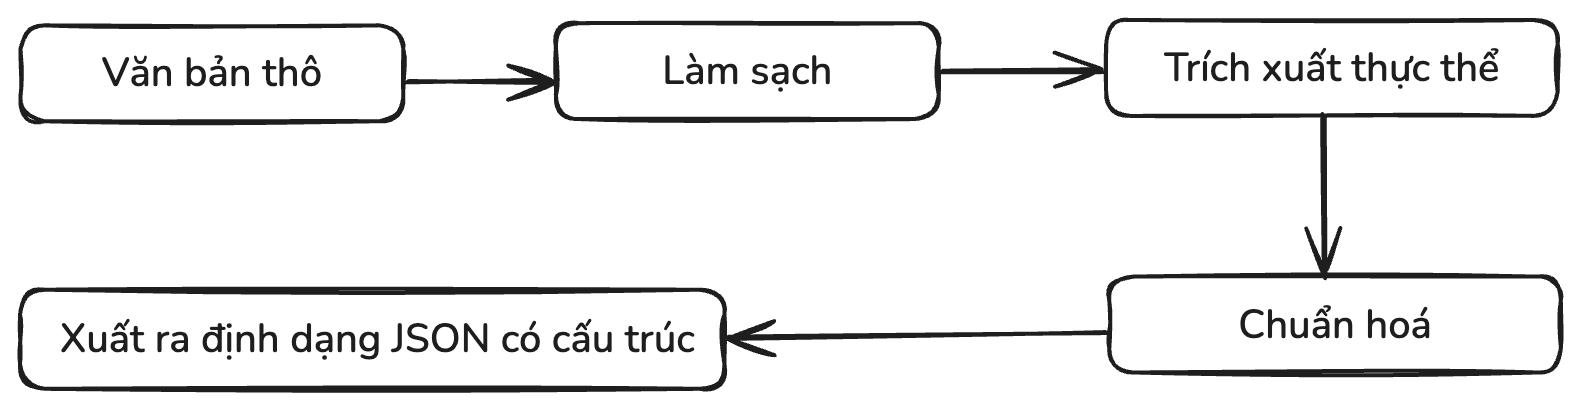
\includegraphics[width=1\linewidth]{img/clean-flow.png}
    \caption{\textit{Quy trình tiền xử lý dữ liệu tổng thể}}
    \label{fig:clean-flow}
\end{figure}

Trong giai đoạn làm sạch, các thao tác chuẩn hóa như đồng bộ mã Unicode, xử lý khoảng trắng, mở rộng từ viết tắt (ví dụ: Sr. → Senior) và xử lý ký tự đặc biệt được thực hiện để tăng tính nhất quán cho dữ liệu đầu vào.

\subsubsection{Đánh giá Chất lượng}
Chất lượng dữ liệu sau tiền xử lý đã được cải thiện một cách đáng kể. Khi đánh giá trên tập kiểm định, quy trình này giúp giảm 12\% tỷ lệ loại nhầm so với các phương pháp chỉ dựa trên đối sánh từ khóa truyền thống. Thêm vào đó, độ đồng thuận giữa kết quả gán nhãn tự động và nhãn của chuyên gia đạt mức cao ($\text{Cohen's } \kappa > 0.85$), khẳng định tính nhất quán và độ tin cậy của quy trình.

Dữ liệu đầu ra có cấu trúc không chỉ là một cơ sở dữ liệu sạch mà còn là một nền tảng ngữ nghĩa phong phú. Nó cho phép hệ thống thực hiện các phân tích sâu hơn như đánh giá mức độ phù hợp theo ngữ cảnh và cấp bậc công việc – những yếu tố phức tạp thường bị các phương pháp truyền thống bỏ qua.

\subsection{Triển khai mô hình minh chứng (Proof-of-Concept)}
Để kiểm chứng tính khả thi của khung kiến trúc đã đề xuất, một mô hình minh chứng (Proof-of-Concept - POC) đã được xây dựng. Mục tiêu của POC không chỉ nhằm xác nhận tính khả thi về mặt kỹ thuật mà còn để đánh giá hiệu năng sơ bộ và trải nghiệm người dùng trong một kịch bản mô phỏng gần với thực tế.

\subsubsection{Kiến trúc hệ thống}
Hệ thống được triển khai dựa trên kiến trúc đa tác nhân dạng mô-đun, nơi các tác nhân chuyên biệt phối hợp với nhau thông qua một quy trình được điều phối tập trung. Thiết kế này đảm bảo các thành phần chức năng được phân tách rõ ràng, tạo điều kiện cho việc kiểm thử độc lập và nâng cấp linh hoạt.

\begin{figure}[H]
    \centering
    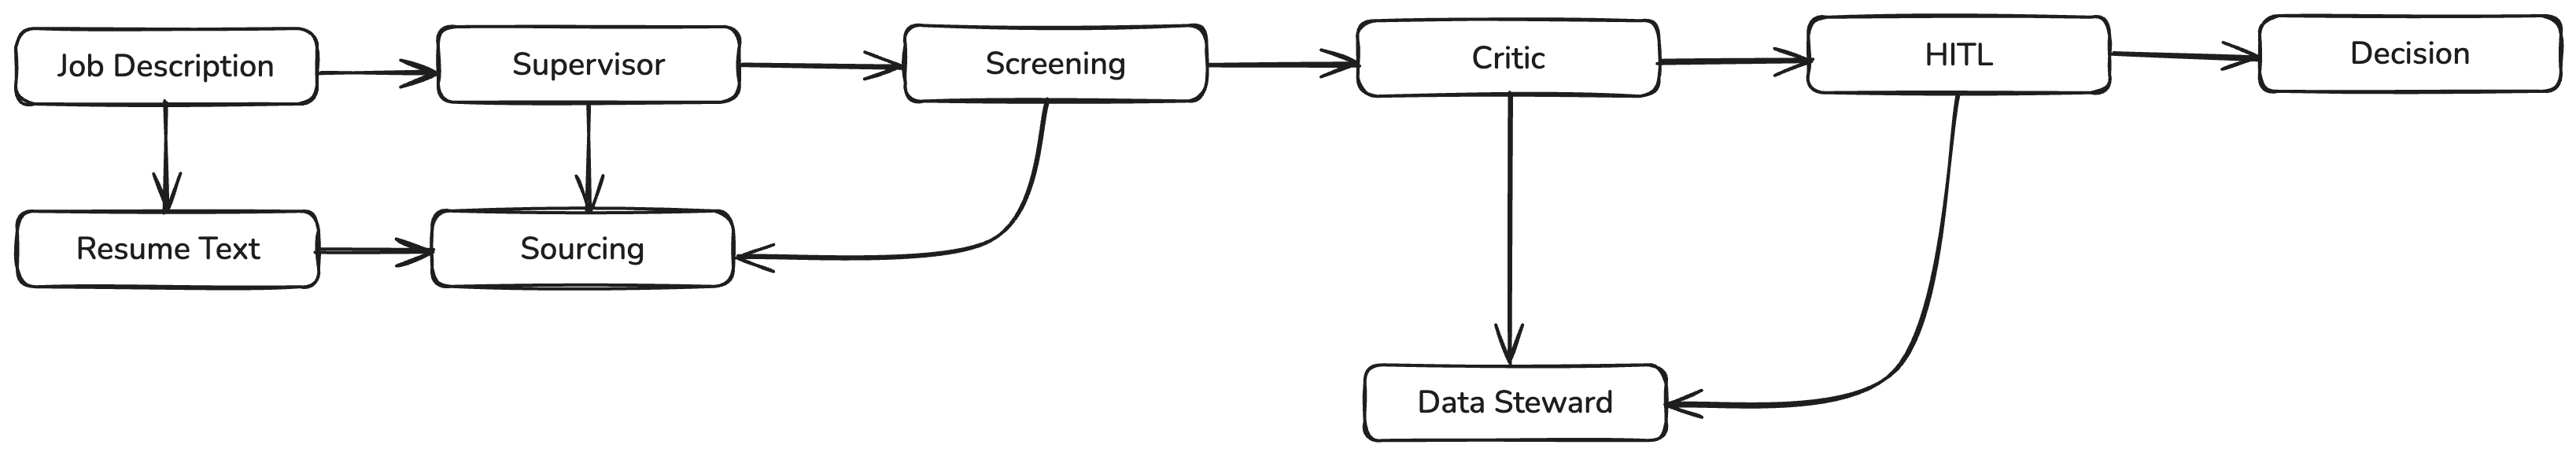
\includegraphics[width=1\linewidth]{img/agents-in-poc.png}
    \caption{\textit{Sơ đồ kiến trúc các tác nhân trong mô hình minh chứng}}
    \label{fig:agents-in-poc}
\end{figure}

Để hiện thực hóa kiến trúc này, một nền tảng công nghệ gọn nhẹ, được tối ưu cho việc xử lý ngữ nghĩa và xây dựng nguyên mẫu nhanh đã được lựa chọn. Các thành phần công nghệ được lựa chọn không chỉ vì hiệu năng mà còn vì khả năng tích hợp cao và sự hỗ trợ mạnh mẽ từ cộng đồng, giúp đẩy nhanh quá trình phát triển.

\begin{longtable}{|
  % Table columns define
  >{\raggedright\arraybackslash}p{0.25\textwidth}|
  >{\raggedright\arraybackslash}p{0.40\textwidth}|
  >{\raggedright\arraybackslash}p{0.35\textwidth}|}
  % Table columns define end here.
  \hline
  % Table header start from here, should modify if needed
  \textbf{Tầng hệ thống} &
  \textbf{Thành phần} &
  \textbf{Mục đích} \\
  \hline
  % Table header end here.
  \endfirsthead

  % No header on continuation pages
  \endhead

  \hline
  \endfoot

  \hline
  \caption{\textit{Các Thành Phần Của Hệ Thống}} \\
  \endlastfoot

  Suy luận LLM &
  OpenAI GPT-4 &
  Ra quyết định phức tạp và xử lý ngôn ngữ tự nhiên \\
  \hline

  So khớp ngữ nghĩa &
  OpenAI text-embedding-3-small (1536 chiều) &
  Phân tích sự tương đồng về kỹ năng \\
  \hline

  Cơ sở dữ liệu vector &
  Milvus Lite &
  Tìm kiếm ngữ nghĩa nội bộ và tính toán độ tương đồng \\
  \hline

  Quản lý trạng thái &
  Redis &
  Phối hợp luồng công việc và lưu trữ tạm thời \\
  \hline

  Giao diện người dùng &
  Chainlit framework &
  Tương tác qua giao diện trò chuyện \\
  \hline

  Kiểm thử &
  pytest với 56 bài kiểm thử đơn vị toàn diện &
  Đảm bảo kiểm thử đầy đủ cho tất cả các thành phần \\
  \hline
\end{longtable}

\subsubsection{Triển khai tác nhân}

Mỗi tác nhân trong hệ thống được triển khai như một đơn vị chức năng độc lập, có vai trò và trách nhiệm rõ ràng, góp phần nâng cao tính minh bạch và khả năng giải trình của toàn bộ quy trình.

\begin{longtable}{|
  % Table columns define
  >{\raggedright\arraybackslash}p{0.17\textwidth}|
  >{\raggedright\arraybackslash}p{0.40\textwidth}|
  >{\raggedright\arraybackslash}p{0.38\textwidth}|}
  % Table columns define end here.
  \hline
  % Table header start from here, should modify if needed
  \textbf{Tác Nhân} & 
  \textbf{Chức Năng Chính} & 
  \textbf{Phương Pháp Thực Hiện} \\
  \hline
  % Table header end here.
  \endfirsthead

  % No header on continuation pages
  \endhead

  \hline
  \endfoot

  \hline
  \caption{\centering\textit{Mô tả chức năng các tác nhân trong hệ thống}}
  \label{tab:agent-functions} \\
  \endlastfoot

  \textbf{Supervisor} & 
  Chuyển mô tả công việc thành tiêu chí cấu trúc; tạo vector kỹ năng (>1,200 kỹ năng) & 
  Dẫn xuất bằng ontology; tổng hợp embedding \\ 
  \hline

  \textbf{Screening} & 
  Chấm điểm ứng viên dựa trên tiêu chí trọng số & 
  Độ tương đồng cosine: kỹ năng (40\%), kinh nghiệm (30\%), học vấn (15\%), lĩnh vực (15\%) \\ 
  \hline

  \textbf{Critic} & 
  Phát hiện thiên kiến và khả năng phù hợp tiềm ẩn & 
  Phân tích chênh lệch, suy diễn chuyển đổi kỹ năng, ánh xạ thay đổi ngành nghề \\ 
  \hline

  \textbf{HITL} & 
  Điều hướng quyết định theo ngưỡng độ tin cậy & 
  Tự động duyệt (>85\%), cần xem xét (65–85\%), chuyển tay (≤65\%) \\ 
  \hline

  \textbf{Data Steward} & 
  Lưu trữ bất biến và theo dõi chỉ số hệ thống & 
  Ghi log bất biến, có thể truy xuất nguồn gốc dữ liệu \\

\end{longtable}

Các tác nhân giao tiếp với nhau thông qua các payload có cấu trúc được quản lý bởi Redis. Cơ chế này đảm bảo trạng thái không ràng buộc (stateless), cho phép hệ thống dễ dàng mở rộng theo chiều ngang khi khối lượng công việc tăng lên.

\subsubsection{Giao diện và trải nghiệm người Dùng}
Giao diện người dùng được phát triển bằng framework Chainlit, mang lại trải nghiệm tương tác trực quan dưới dạng hội thoại, rất phù hợp với bối cảnh làm việc của chuyên viên nhân sự. Thay vì các biểu mẫu phức tạp, người dùng có thể tương tác với hệ thống một cách tự nhiên.

Luồng đánh giá của người dùng được thiết kế đơn giản và minh bạch:
\begin{itemize}[topsep=0pt, itemsep=4pt, leftmargin=40pt]
    \item \textbf{Khởi tạo}: Người dùng tải lên mô tả công việc và các hồ sơ ứng viên cần đánh giá. Hệ thống cũng cung cấp chế độ demo với dữ liệu mẫu.
    \item \textbf{Xử lý}: Hệ thống hiển thị tiến trình xử lý của từng tác nhân theo thời gian thực, giúp người dùng nắm bắt được trạng thái công việc.
    \item \textbf{Trình bày kết quả}: Kết quả cuối cùng được trình bày rõ ràng, bao gồm điểm số, độ tin cậy, một bản đồ kỹ năng trực quan, các ghi chú về thiên vị (nếu có), và đề xuất hành động tiếp theo. Giao diện được thiết kế đáp ứng tốt (responsive) trên cả máy tính và thiết bị di động.
\end{itemize}

\subsubsection{Kiểm thử và xác minh}
Hệ thống được phát triển theo phương pháp ưu tiên kiểm thử (test-driven development), với một bộ gồm 56 bài kiểm thử đơn vị cùng các kịch bản kiểm thử tích hợp và hiệu năng. Để xác minh khả năng xử lý trong các tình huống thực tế, một số kịch bản điển hình đã được thực thi:

\begin{longtable}{|
  % Table columns define
  >{\raggedright\arraybackslash}p{0.35\textwidth}|
  >{\raggedright\arraybackslash}p{0.30\textwidth}|
  >{\raggedright\arraybackslash}p{0.30\textwidth}|}
  % Table columns define end here.
  \hline
  % Table header start from here, should modify if needed
  \textbf{Tình Huống} &
  \textbf{Kết Quả} &
  \textbf{Nhận Định Chính} \\
  \hline
  % Table header end here.
  \endfirsthead

  % No header on continuation pages
  \endhead

  \hline
  \endfoot

  \hline
  \caption{\centering\textit{Một số kịch bản kiểm thử điển hình và nhận định}}
  \label{tab:test-scenarios-summary} \\
  \endlastfoot

  Phù hợp hoàn hảo (Senior Python Dev, 7 năm) &
  Tin cậy 95\%; tự động duyệt trong 3–4 phút &
  Hệ thống đạt độ chính xác như kỳ vọng \\
  \hline

  Tiềm năng ẩn (Chuyển từ Tài chính → Data) &
  Tin cậy 78\% sau hiệu chỉnh; đề xuất xem xét &
  Nhận diện chính xác kỹ năng chuyển đổi \\
  \hline

  Từ chối rõ ràng (Junior so với Senior DevOps) &
  Tin cậy 35\%; tự động từ chối trong 2–3 phút &
  Giảm tải tính toán nhờ loại sớm \\

\end{longtable}

Kết quả kiểm thử cho thấy thời gian phản hồi của hệ thống ổn định trong khoảng 3-5 phút cho mỗi hồ sơ, ngay cả khi xử lý đồng thời nhiều yêu cầu, chứng tỏ kiến trúc được lựa chọn có tính ổn định và sẵn sàng cho môi trường thực tế.

\subsubsection{Kết quả triển khai}
Kết quả kiểm thử cho thấy thời gian phản hồi của hệ thống ổn định trong khoảng 3-5 phút cho mỗi hồ sơ, ngay cả khi xử lý đồng thời nhiều yêu cầu, chứng tỏ kiến trúc được lựa chọn có tính ổn định và sẵn sàng cho môi trường thực tế.

\begin{longtable}{|
  % Table columns define
  >{\raggedright\arraybackslash}p{0.25\textwidth}|
  >{\raggedright\arraybackslash}p{0.35\textwidth}|
  >{\raggedright\arraybackslash}p{0.35\textwidth}|}
  % Table columns define end here.
  \hline
  % Table header start from here, should modify if needed
  \textbf{Chỉ Số} &
  \textbf{Kết Quả} &
  \textbf{Ý Nghĩa} \\
  \hline
  % Table header end here.
  \endfirsthead

  % No header on continuation pages
  \endhead

  \hline
  \endfoot

  \hline
  \caption{\centering\textit{Tổng kết các kết quả triển khai mô hình minh chứng}}
  \label{tab:ket-qua-minh-chung} \\
  \endlastfoot

  Tốc độ xử lý &
  3–5 phút mỗi lượt đánh giá &
  Phù hợp với yêu cầu thực tiễn trong tuyển dụng \\
  \hline

  Độ tin cậy &
  Tỷ lệ kiểm thử thành công 100\% &
  Kiến trúc hệ thống ổn định \\
  \hline

  Tỷ lệ phát hiện thiên kiến &
  25\% hồ sơ được gắn cờ thiên kiến &
  Thiết kế hướng đến công bằng \\
  \hline

  Nhận diện chuyển đổi kỹ năng &
  Ghi nhận chuyển đổi từ tài chính sang công nghệ &
  Chứng minh hiệu quả của mô hình ngữ nghĩa so với từ khóa \\
  \hline

  Phản hồi người dùng (demo) &
  Tích cực; được đánh giá “sẵn sàng triển khai” &
  Giao diện phù hợp triển khai thử nghiệm \\

\end{longtable}

Những thành tựu nổi bật của giai đoạn triển khai bao gồm việc tích hợp thành công năm tác nhân trong một quy trình thống nhất, chứng minh hiệu quả của cơ chế so khớp ngữ nghĩa, và đặc biệt là khả năng nhận diện các ứng viên phi truyền thống. Mô hình minh chứng, với bộ kiểm thử tự động và kịch bản demo hoàn chỉnh, đã đặt một nền tảng vững chắc cho giai đoạn đánh giá định lượng tiếp theo.

\subsubsection{Kết luận}
Việc triển khai thành công mô hình minh chứng đã xác nhận tính khả thi của việc áp dụng kiến trúc đa tác nhân vào bài toán tuyển dụng. Hệ thống không chỉ mang lại hiệu quả rõ rệt về tính công bằng, minh bạch và hiệu suất mà còn duy trì một trải nghiệm người dùng thân thiện, hiện đại. Nền tảng này đã sẵn sàng để được kiểm chứng hiệu quả một cách định lượng trong các bối cảnh tuyển dụng thực tế.

\subsection{Đánh giá}
Mục này trình bày phương pháp luận và thiết kế thực nghiệm được sử dụng để đánh giá hiệu quả của hệ thống đa tác nhân được đề xuất.

\subsubsection{Câu hỏi nghiên cứu}
Trọng tâm của quá trình đánh giá là kiểm chứng giả thuyết nghiên cứu chính: Liệu kiến trúc đa tác nhân, với khả năng phân tích ngữ nghĩa, có thể giảm thiểu một cách đáng kể tỷ lệ FRR so với các hệ thống ATS truyền thống vốn chỉ dựa trên đối sánh từ khóa hay không?.

\subsubsection{Thiết kế đánh giá}
Để trả lời câu hỏi trên, một thực nghiệm có đối chứng được thiết kế và triển khai theo một quy trình chặt chẽ.

\begin{enumerate}[topsep=0pt, itemsep=4pt, leftmargin=40pt, label=\arabic*.]
    \item \textbf{Đo lường hiệu suất nền (Baseline)}: Đầu tiên, Tỷ lệ Loại nhầm (FRR) của một hệ thống ATS mô phỏng, vận hành theo cơ chế đối sánh từ khóa truyền thống, được tính toán để làm mốc so sánh.
    \item \textbf{Can thiệp và đo lường}: Tiếp theo, cùng một tập dữ liệu sẽ được xử lý bởi hệ thống đa tác nhân được đề xuất, vốn tích hợp các cơ chế phân tích ngữ nghĩa và đánh giá đa chiều.
    \item \textbf{Phân tích so sánh}: Cuối cùng, kết quả FRR từ hai hệ thống được đối chiếu bằng các kiểm định thống kê để xác định mức độ ý nghĩa của sự khác biệt, với ngưỡng ý nghĩa được đặt ở $\alpha=0.05$. Phép phân tích cũng bao gồm việc ước lượng kích thước hiệu ứng để đánh giá tác động thực tiễn của giải pháp.
\end{enumerate}

\subsubsection{Định nghĩa chỉ số}
Chỉ số hiệu suất cốt lõi được sử dụng trong đánh giá là \textbf{Tỷ lệ Loại nhầm (False Rejection Rate - FRR)}. Chỉ số này đo lường phần trăm số ứng viên đủ điều kiện nhưng lại bị hệ thống sàng lọc loại bỏ một cách sai lầm. Công thức được định nghĩa như sau:

$$
\text{FRR} = \frac{\text{Số ứng viên đủ điều kiện bị hệ thống loại}}{\text{Tổng số ứng viên đủ điều kiện}}
$$

FRR được chọn làm chỉ số chính vì nó phản ánh trực tiếp rủi ro bỏ lỡ nhân tài—một trong những tổn thất chi phí cơ hội lớn nhất trong quy trình tuyển dụng hiện đại.

\subsubsection{Tiêu chí đánh giá ứng viên}
Để đảm bảo tính nhất quán và khách quan, một khung tiêu chí có trọng số đã được áp dụng thống nhất cho cả hai hệ thống. Một ứng viên được xem là "đủ điều kiện" khi đạt tổng điểm từ 31\% trở lên, và được đưa vào danh sách rút gọn nếu vượt qua 50\%. Các trọng số phản ánh mức độ quan trọng tương đối của từng yếu tố trong bối cảnh tuyển dụng ngành công nghệ.

\begin{longtable}{|
  % Table columns define
  >{\raggedright\arraybackslash}p{0.60\textwidth}|
  >{\centering\arraybackslash}p{0.30\textwidth}|}
  % Table columns define end here.
  \hline
  % Table header start from here, should modify if needed
  \textbf{Tiêu chí} &
  \textbf{Trọng số} \\
  \hline
  % Table header end here.
  \endfirsthead

  % No header on continuation pages
  \endhead

  \hline
  \endfoot

  \hline
  \caption{\centering\textit{Các tiêu chí đánh giá ứng viên và trọng số tương ứng}}
  \label{tab:candidate-evaluation-criteria} \\
  \endlastfoot

  Mức độ phù hợp kỹ năng & 40\% \\
  \hline

  Kinh nghiệm & 30\% \\
  \hline

  Học vấn liên quan & 15\% \\
  \hline

  Lĩnh vực chuyên môn & 15\% \\

\end{longtable}

\subsubsection{Cấu hình thí nghiệm}

Thí nghiệm được thực hiện trên tập dữ liệu gồm 1,182 hồ sơ thuộc lĩnh vực công nghệ, trong đó có 885 hồ sơ đã được chuyên gia gán nhãn thủ công để làm dữ liệu chuẩn (ground-truth). Hai hệ thống được đưa vào so sánh bao gồm: (a) một hệ thống đối sánh từ khóa cơ bản và (b) hệ thống đa tác nhân tích hợp phân tích ngữ nghĩa. Để đảm bảo tính công bằng, cả hai hệ thống đều sử dụng chung một bộ tiêu chí đánh giá và quy trình thử nghiệm.

Về mặt phân tích, nghiên cứu sử dụng hệ số h của Cohen để lượng hóa kích thước hiệu ứng và tính toán khoảng tin cậy 95\% nhằm gia tăng độ tin cậy của kết quả. Mức ý nghĩa thống kê được xác định ở ngưỡng $p<0.05$. Thiết kế này cho phép quy kết một cách hợp lý rằng mọi cải thiện quan sát được về FRR đều đến từ năng lực vượt trội của kiến trúc đa tác nhân, đồng thời giảm thiểu các yếu tố gây nhiễu từ dữ liệu hay phương pháp luận.

\subsection{Kết quả}
Mục này trình bày các kết quả thực nghiệm từ việc so sánh hiệu suất giữa hệ thống đa tác nhân được đề xuất và hệ thống ATS nền tảng. Các phát hiện khẳng định hiệu quả của kiến trúc mới trong việc giảm thiểu tỷ lệ loại nhầm và nâng cao độ chính xác tổng thể.

\subsubsection{Phát hiện chính}
Kết quả cốt lõi của nghiên cứu cho thấy việc triển khai hệ thống sàng lọc đa tác nhân đã giúp giảm Tỷ lệ Loại nhầm (FRR) một cách đáng kể. Cụ thể, FRR đã giảm từ \textbf{30.8\%} ở hệ thống ATS nền tảng dựa trên từ khóa xuống chỉ còn \textbf{7.4\%} ở hệ thống đề xuất. \textbf{Mức cải thiện tương đối đạt 76\%} này không chỉ có ý nghĩa về mặt thống kê ($p<0.05$) mà còn có tác động lớn trong thực tiễn, được thể hiện qua chỉ số kích thước hiệu ứng ở mức trung bình-lớn ($\text{Cohen's h}=0.625$).

\subsubsection{Hiệu suất so sánh}
Để làm rõ hơn sự khác biệt, bảng dưới đây trình bày số liệu so sánh hiệu suất chi tiết giữa hai hệ thống.

\begin{longtable}{|
  % Table columns define
  >{\raggedright\arraybackslash}p{0.18\textwidth}|
  >{\raggedright\arraybackslash}p{0.18\textwidth}|
  >{\raggedright\arraybackslash}p{0.18\textwidth}|
  >{\raggedright\arraybackslash}p{0.13\textwidth}|
  >{\raggedright\arraybackslash}p{0.12\textwidth}|
  >{\raggedright\arraybackslash}p{0.16\textwidth}|}
  % Table columns define end here.
  \hline
  % Table header start from here, should modify if needed
  \textbf{Hệ thống} &
  \textbf{Số ứng viên sàng lọc} &
  \textbf{Ứng viên đủ điều kiện} &
  \textbf{Loại nhầm} &
  \textbf{FRR} &
  \textbf{Độ chính xác tổng thể} \\
  \hline
  % Table header end here.
  \endfirsthead

  % No header on continuation pages
  \endhead

  \hline
  \endfoot

  \hline
  \caption{\centering\textit{So sánh hiệu suất giữa hệ thống nền tảng và hệ thống đa tác nhân}}
  \label{tab:performance-comparison} \\
  \endlastfoot

  Nền tảng &
  971 &
  380 &
  117 &
  \textbf{30.8\%} &
  88.0\% \\
  \hline

  Đa tác nhân &
  885 &
  608 &
  45 &
  \textbf{7.4\%} &
  94.9\% \\

\end{longtable}

Dữ liệu cho thấy hệ thống đa tác nhân, dù xử lý ít hồ sơ hơn, lại xác định được số lượng ứng viên đủ điều kiện cao hơn đáng kể và giảm mạnh các trường hợp loại sai. Điều này trực tiếp góp phần nâng cao độ chính xác tổng thể của quy trình sàng lọc.

\subsubsection{Xác nhận thống kê}

Phân tích sâu hơn về mặt thống kê cho thấy Tỷ lệ Loại nhầm (FRR) đã giảm tuyệt đối 23.4 điểm phần trăm. Khoảng tin cậy 95\% của mức giảm này dao động từ 18.3\% đến 28.5\%, xác nhận rằng sự cải thiện không phải do ngẫu nhiên. Chỉ số kích thước hiệu ứng Cohen's h đạt 0.625, một lần nữa khẳng định rằng mức độ cải thiện là đáng kể và có ý nghĩa thực tiễn, củng cố độ tin cậy và tiềm năng ứng dụng của hệ thống.

\subsubsection{Tác động kinh doanh}
Trên quy mô lớn, những cải tiến về mặt kỹ thuật này mang lại giá trị kinh doanh rõ rệt. Hệ thống có khả năng ngăn chặn trung bình 72 trường hợp loại nhầm trong mỗi đợt tuyển dụng, giúp tăng 60\% số lượng ứng viên chất lượng được xác định. Hơn nữa, nhờ khả năng phân tích kỹ năng chuyển đổi, hệ thống còn phát hiện thêm khoảng 27 ứng viên tiềm năng mà các phương pháp truyền thống thường bỏ sót.

Khi áp dụng cho một quy trình tuyển dụng 10,000 ứng viên mỗi năm, số trường hợp loại sai có thể giảm từ 3,080 xuống chỉ còn 740. Những con số này cung cấp một cơ sở thuyết phục để các tổ chức xem xét và áp dụng kiến trúc đa tác nhân vào thực tiễn.

\subsubsection{Thảo luận}
Kết quả thực nghiệm đã xác thực một cách thuyết phục giả thuyết nghiên cứu: kiến trúc AI đa tác nhân có thể giảm thiểu đáng kể Tỷ lệ Loại nhầm (False Rejection Rate - FRR) trong quy trình sàng lọc ứng viên so với các hệ thống truyền thống. Mức giảm FRR lên đến 76\%, cùng với kích thước hiệu ứng ở mức trung bình-lớn ($\text{Cohen's } h=0.625$), không chỉ có ý nghĩa về mặt thống kê ($p<0.05$) mà còn khẳng định giá trị tác động trên thực tiễn của giải pháp.

Phân tích sâu hơn các kết quả đã cho thấy những phát hiện quan trọng. Mức FRR 30.8\% của hệ thống nền tảng hoàn toàn tương thích với các lo ngại đã được ghi nhận trong nhiều báo cáo uy tín của ngành, như của Trường Kinh doanh Harvard (2021), chứng tỏ vấn đề mà luận văn giải quyết là có thật và cấp thiết. Hệ thống đa tác nhân đề xuất không chỉ khắc phục điểm yếu này mà còn gần như nhân đôi tỷ lệ nhận diện ứng viên đủ điều kiện, từ 39.1\% lên 68.7\%. Đặc biệt, năng lực khớp ngữ nghĩa của hệ thống đã cho phép phát hiện 27 ứng viên tiềm năng vốn rất dễ bị các hệ thống truyền thống bỏ qua. Khi đặt trong bối cảnh các nghiên cứu trước đây, vốn báo cáo mức giảm FRR chỉ trong khoảng 25-40\%, con số 76\% mà hệ thống này đạt được thể hiện một bước tiến vượt trội, cho thấy ưu thế của khung phân tích ngữ nghĩa kết hợp đa tác nhân.

Tuy nhiên, dù kết quả rất khả quan, nghiên cứu vẫn tồn tại một số giới hạn cần được nhìn nhận một cách khách quan. Thứ nhất, việc đánh giá được thực hiện trên một tập dữ liệu chuyên ngành (công nghệ), điều này có thể ảnh hưởng đến khả năng khái quát hóa kết quả sang các lĩnh vực khác. Thêm vào đó, thử nghiệm được tiến hành tại một thời điểm duy nhất và chưa có các kiểm chứng về hiệu suất theo thời gian. Cuối cùng, dù đã sử dụng dữ liệu chuẩn do chuyên gia gán nhãn, độ chính xác của hệ thống so với các quyết định tuyển dụng trong thực tế vẫn cần được xác minh thêm trong các nghiên cứu tương lai.

Vượt trên những con số thống kê, tác động thực tiễn của nghiên cứu là rất rõ ràng. Việc giảm đáng kể FRR và tăng cường khả năng nhận diện đúng ứng viên là một đóng góp trực tiếp vào việc nâng cao tính công bằng và hiệu quả trong tuyển dụng. Những cải tiến này mang lại giá trị có thể đo lường được cho tổ chức, đồng thời cho thấy tiềm năng to lớn của hệ thống sàng lọc dựa trên tác nhân thông minh trong việc hiện đại hóa quy trình thu hút nhân tài.

\subsection{Tổng kết chương}
Chương 5 đã trình bày một cách hệ thống quá trình triển khai và kiểm nghiệm thực nghiệm kiến trúc đa tác nhân, qua đó cung cấp những bằng chứng định lượng vững chắc để xác thực cho giả thuyết nghiên cứu. Mục tiêu xuyên suốt của chương là chuyển hóa bản thiết kế kiến trúc từ Chương 4 thành một mô hình minh chứng (Proof-of-Concept) hoạt động và đánh giá hiệu quả của nó một cách khoa học.

Quá trình được bắt đầu bằng việc chuẩn bị và tiền xử lý một bộ dữ liệu chuyên ngành gồm 1,182 hồ sơ, đảm bảo dữ liệu đầu vào có cấu trúc, giàu ngữ nghĩa và được gán nhãn bởi chuyên gia. Giai đoạn này không chỉ tạo ra một nền tảng dữ liệu chất lượng cao mà còn chứng minh rằng quy trình xử lý thông minh có thể cải thiện đáng kể độ chính xác ngay từ bước đầu. Tiếp đó, một mô hình minh chứng đã được triển khai thành công, xác nhận tính khả thi về mặt kỹ thuật của kiến trúc đa tác nhân dạng mô-đun. Việc tích hợp các công nghệ như LLM (GPT-4) và cơ sở dữ liệu vector (Milvus Lite) đã hiện thực hóa một quy trình phối hợp nhịp nhàng giữa các tác nhân chuyên biệt, từ sàng lọc, phản biện đến tương tác có con người trong vòng lặp.

Trọng tâm của chương là cuộc thí nghiệm có đối chứng, được thiết kế chặt chẽ để so sánh hiệu suất giữa hệ thống đa tác nhân và một hệ thống ATS truyền thống dựa trên từ khóa. Kết quả thực nghiệm đã khẳng định một cách thuyết phục giá trị của giải pháp đề xuất. Cụ thể, hệ thống đã giảm thiểu Tỷ lệ Loại nhầm (False Rejection Rate - FRR) một cách ngoạn mục, từ 30.8\% ở hệ thống nền tảng xuống chỉ còn 7.4\%, tương đương mức cải thiện tương đối lên đến 76\%. Sự cải thiện này không chỉ có ý nghĩa sâu sắc về mặt thống kê ($p<0.05$) mà còn mang lại tác động lớn trong thực tiễn, được xác thực qua chỉ số kích thước hiệu ứng ở mức trung bình-lớn (Cohen's $h=0.625$).

Phân tích sâu hơn cho thấy hệ thống không chỉ giảm sai sót mà còn nâng cao đáng kể độ chính xác tổng thể (từ 88.0\% lên 94.9\%) và gần như nhân đôi khả năng nhận diện các ứng viên thực sự đủ điều kiện. Những phát hiện này cung cấp bằng chứng mạnh mẽ rằng việc chuyển đổi từ cơ chế đối sánh từ khóa tĩnh sang một kiến trúc phân tích ngữ nghĩa, đa chiều là một hướng đi vượt trội. Mặc dù nghiên cứu vẫn tồn tại một số giới hạn nhất định, các kết quả định lượng thu được đã đặt một nền tảng thực nghiệm vững chắc, không chỉ xác thực hiệu quả của giải pháp mà còn mở ra những tiềm năng ứng dụng to lớn trong việc hiện đại hóa quy trình thu hút nhân tài.

\newpage
\phantomsection
\titlespacing{\section}{0pt}{0pt}{30pt} %heading 1
\titleformat{\section}{\centering\fontsize{28pt}{8pt}\bfseries}{}{0pt}{%
    {}%
    {}%
}
\addcontentsline{toc}{section}{\numberline{}KẾT LUẬN}
\section*{KẾT LUẬN}
Luận văn này đã thực hiện nghiên cứu, thiết kế và kiểm nghiệm một kiến trúc đa tác nhân (Multi-Agent System - MAS) cho bài toán sàng lọc ứng viên trong quản lý nhân sự. Xuất phát từ thực trạng các Hệ thống Theo dõi Ứng viên (ATS) truyền thống, với sự phụ thuộc vào cơ chế đối sánh từ khóa tĩnh, đang gây ra một Tỷ lệ Loại nhầm (False Rejection Rate - FRR) ở mức báo động từ 12\% đến 35\%, nghiên cứu đã đề xuất một giải pháp thay thế nhằm khắc phục những yếu điểm mang tính hệ thống này. Kiến trúc được đề xuất chuyển đổi trọng tâm từ việc so khớp từ vựng sang thấu hiểu ngữ nghĩa, kết hợp với cơ chế giám sát của con người trong vòng lặp (Human-in-the-Loop - HITL) để đảm bảo tính chính xác, công bằng và hiệu quả.

Thông qua việc triển khai một mô hình minh chứng (Proof-of-Concept) và thực hiện một thí nghiệm có đối chứng, luận văn đã cung cấp những bằng chứng thực nghiệm thuyết phục, cho thấy hệ thống đề xuất có khả năng giảm thiểu FRR một cách đáng kể từ 30.8\% xuống chỉ còn 7.4\%, tương đương mức cải thiện 76\%. Kết quả này không chỉ xác thực giả thuyết nghiên cứu mà còn khẳng định tiềm năng to lớn của việc ứng dụng các tác nhân AI thông minh vào việc hiện đại hóa quy trình thu hút nhân tài.

Các đóng góp chính của luận văn bao gồm
\begin{enumerate}[topsep=0pt, itemsep=4pt, leftmargin=40pt, label=\arabic*.]
    \item \textbf{Phân tích và lượng hóa các khiếm khuyết của ATS truyền thống}: Luận văn đã phân tích sâu sắc và cung cấp bằng chứng thực nghiệm về ba khiếm khuyết kiến trúc cốt lõi của các hệ thống ATS hiện hành: sự phụ thuộc vào từ khóa tĩnh, thuật toán đồng nhất hóa gây thiên vị, và cơ chế chấm điểm "hộp đen" thiếu minh bạch.
    \item \textbf{Thiết kế một kiến trúc đa tác nhân chuyên biệt và toàn diện}: Đề xuất một kiến trúc MAS dạng mô-đun với sáu tác nhân chuyên biệt (Supervisor, Sourcing, Screening, Critic, HITL, Data-Steward), mỗi tác nhân đảm nhận một vai trò rõ ràng, phối hợp nhịp nhàng để tạo ra một quy trình sàng lọc minh bạch, có khả năng giải trình và kiểm toán.
    \item \textbf{Hiện thực hóa cơ chế đánh giá dựa trên năng lực thực sự}: Thay vì chỉ dựa vào từ khóa, hệ thống đã triển khai thành công các cơ chế phân tích ngữ nghĩa (Meaning Matcher) và diễn giải lộ trình sự nghiệp (Career Translator), cho phép nhận diện các kỹ năng có thể chuyển đổi và đánh giá đúng tiềm năng của các ứng viên có nền tảng phi truyền thống.
    \item \textbf{Tích hợp cơ chế Human-in-the-Loop (HITL) một cách thông minh}: Thiết kế một quy trình HITL được kích hoạt có chọn lọc dựa trên điểm tự tin, vốn được tính từ mức độ đồng thuận giữa hai tác nhân có góc nhìn đối trọng (Screening và Critic). Cách tiếp cận này giúp cân bằng tối ưu giữa hiệu suất xử lý tự động và sự giám sát chuyên môn của con người.
    \item \textbf{Cung cấp bằng chứng thực nghiệm về hiệu quả vượt trội}: Kết quả kiểm nghiệm đã chứng minh hệ thống đề xuất không chỉ giảm 76\% Tỷ lệ Loại nhầm mà còn tăng độ chính xác tổng thể của quy trình sàng lọc từ 88.0\% lên 94.9\%, đồng thời xác định được nhiều hơn 60\% số lượng ứng viên chất lượng.
\end{enumerate}

Mặc dù các kết quả đạt được rất khả quan, nghiên cứu vẫn tồn tại một số giới hạn cần được nhìn nhận một cách khách quan để định hướng cho các công trình trong tương lai:
\begin{itemize}[topsep=0pt, itemsep=4pt, leftmargin=40pt]
    \item \textbf{Phạm vi dữ liệu}: Nghiên cứu được thực hiện trên một bộ dữ liệu chuyên ngành công nghệ. Điều này có thể ảnh hưởng đến khả năng khái quát hóa kết quả sang các lĩnh vực khác với các bộ kỹ năng và cấu trúc hồ sơ đặc thù.
    \item \textbf{Đánh giá tại một thời điểm}: Thí nghiệm được tiến hành tại một thời điểm duy nhất. Hiệu suất của hệ thống, đặc biệt là khả năng học hỏi và thích ứng từ các phản hồi HITL, cần được kiểm chứng thông qua các nghiên cứu theo chiều dọc (longitudinal studies) kéo dài qua nhiều chu kỳ tuyển dụng.
    \item \textbf{Xác thực trong môi trường thực tế}: Dù dữ liệu được gán nhãn bởi chuyên gia, việc đối chiếu kết quả của hệ thống với các quyết định tuyển dụng thực tế trong một môi trường doanh nghiệp sẽ cung cấp một thước đo xác thực và toàn diện hơn về tác động kinh doanh.
\end{itemize}
    
Dựa trên các kết quả đã đạt được và những hạn chế còn tồn tại, các hướng phát triển tiếp theo cho nghiên cứu này bao gồm:
\begin{itemize}[topsep=0pt, itemsep=4pt, leftmargin=40pt]
    \item \textbf{Mở rộng và tinh chỉnh cho các lĩnh vực khác}: Áp dụng và điều chỉnh mô hình cho các ngành nghề khác như tài chính, y tế, hoặc sản xuất, đòi hỏi việc xây dựng các ontology kỹ năng và mô hình diễn giải kinh nghiệm chuyên biệt.
    \item \textbf{Tăng cường khả năng học hỏi liên tục và cá nhân hóa}: Nghiên cứu các thuật toán học tập trực tuyến (online learning) để hệ thống có thể cập nhật và cá nhân hóa các tiêu chí đánh giá theo thời gian thực dựa trên phản hồi của từng nhà tuyển dụng.
    \item \textbf{Phát triển giao diện tương tác và giải trình nâng cao}: Xây dựng các giao diện trực quan hóa, cho phép chuyên viên nhân sự dễ dàng "hỏi-đáp" và khám phá lý do đằng sau các quyết định của AI, từ đó tăng cường sự tin tưởng và hợp tác giữa người và máy.
    \item \textbf{Tích hợp toàn diện vào hệ sinh thái HRM}: Phát triển các API mạnh mẽ để tích hợp liền mạch hệ thống đa tác nhân với các phần mềm Quản lý Nguồn nhân lực (HRM) hiện có, tạo ra một luồng dữ liệu tuyển dụng thông suốt từ đầu đến cuối.
\end{itemize}
    
\newpage
\phantomsection
\addcontentsline{toc}{section}{\numberline{}TÀI LIỆU THAM KHẢO}
\section*{TÀI LIỆU THAM KHẢO}
\begin{enumerate}[itemsep=5pt]
  \item OECD (2023), \href{https://doi.org/10.1787/08785bba-en}{\textit{OECD Employment Outlook 2023: Artificial Intelligence and the Labour Market}}, OECD Publishing, Paris.
  \item Fuller, J., & Raman, M. (2022). \href{https://www.hbs.edu/managing-the-future-of-work/Documents/research/hiddenworkers09032021.pdf}{\textit{Hidden Workers: Untapped Talent}}. Harvard Business School Project on Managing the Future of Work.
  \item GoodTime. (2024). \href{https://goodtime.io/resources/thank-you-report-hiring-insights-2025/lessons-from-2024/}{\textit{2025 Hiring Insights Report}}.
  \item AMS. (2023). \href{https://www.weareams.com/p/102ii9p/time-to-hire-now-averages-43-days-and-is-increasing/}{\textit{Time to hire now averages 43 days and is increasing}}.
  \item Vaswani, A., Shazeer, N., Parmar, N., Uszkoreit, J., Jones, L., Gomez, A. N., Kaiser, L., & Polosukhin, I. (2017). \href{https://arxiv.org/abs/1706.03762}{\textit{Attention Is All You Need}}.
  \item Shoham, Y., & Leyton-Brown, K. (2009). \href{http://www.masfoundations.org/}{\textit{Multiagent Systems: Algorithmic, Game-Theoretic, and Logical Foundations}}. Cambridge University Press.
  \item Kubera, Y., Mathieu, P., & Picault, S. (2010). \href{https://hal.science/hal-00584364}{\textit{Everything can be Agent!}}. Proc. AAMAS 2010, 1547–1548.
  \item Wooldridge, M. (2002). \href{https://www.wiley.com/en-be/An+Introduction+to+MultiAgent+Systems\%2C+2nd+Edition-p-9780470519462}{\textit{An Introduction to MultiAgent Systems}}. John Wiley \& Sons. p. 366.
  \item Powers, D. M. W. (2011). \href{https://web.archive.org/web/20191114213255/https://www.flinders.edu.au/science_engineering/fms/School-CSEM/publications/tech_reps-research_artfcts/TRRA_2007.pdf}{\textit{Evaluation: From Precision, Recall and F-Measure to ROC, Informedness, Markedness \& Correlation}}. Journal of Machine Learning Technologies, 2(1), 37–63.
  \item National Institute of Standards and Technology (NIST). (n.d.). \href{https://csrc.nist.gov/glossary/term/false_reject_rate}{\textit{False Reject Rate (FRR)}}. Computer Security Resource Center Glossary.
  \item National Center for Biotechnology Information (NCBI). (n.d.). \href{https://pmc.ncbi.nlm.nih.gov/articles/PMC1447545/}{\textit{Evaluation: From Precision, Recall and F‑Measure to ROC, Informedness, Markedness & Correlation}}. NCBI PubMed Central, PMC1447545.
  \item Purcell, K. (2025). \href{https://www.jobscan.co/blog/fortune-500-use-applicant-tracking-systems/}{\textit{Do Fortune 500 Companies Use Applicant Tracking Systems?}}.
  \item Greenhouse Software, Inc. (2024). \href{https://www.prnewswire.com/news-releases/greenhouse-software-recognized-in-2024-gartner-market-guide-for-talent-acquisition-recruiting-technologies-302106647.html}{\textit{Greenhouse Software Recognized in 2024 Gartner® Market Guide for Talent Acquisition (Recruiting) Technologies}}.
  \item Verity AI. (n.d.). \href{https://verityai.co/blog/harvard-study-ai-rejects-qualified-candidates}{\textit{Harvard Study Reveals AI Rejects Over 70\% of Qualified Candidates}}.
\end{enumerate}
\cleardoublepage
\end{document}
